\documentclass[
12pt, % The default document font size, options: 10pt, 11pt, 12pt
onehalfspacing, % Single line spacing, alternatives: onehalfspacing or doublespacing
nohyperref, % Uncomment to not load the hyperref package
headsepline, % Uncomment to get a line under the header
chapterinoneline, % Uncomment to place the chapter title next to the number on one line
]{MastersDoctoralThesis} % The class file specifying the document structure
%% maxwidth is the original width if it is less than linewidth
%% otherwise use linewidth (to make sure the graphics do not exceed the margin)
\makeatletter
\def\maxwidth{ %
  \ifdim\Gin@nat@width>\linewidth
    \linewidth
  \else
    \Gin@nat@width
  \fi
}
\makeatother
\usepackage[]{color}
\definecolor{fgcolor}{rgb}{0.345, 0.345, 0.345}
\newcommand{\hlnum}[1]{\textcolor[rgb]{0.686,0.059,0.569}{#1}}%
\newcommand{\hlstr}[1]{\textcolor[rgb]{0.192,0.494,0.8}{#1}}%
\newcommand{\hlcom}[1]{\textcolor[rgb]{0.678,0.584,0.686}{\textit{#1}}}%
\newcommand{\hlopt}[1]{\textcolor[rgb]{0,0,0}{#1}}%
\newcommand{\hlstd}[1]{\textcolor[rgb]{0.345,0.345,0.345}{#1}}%
\newcommand{\hlkwa}[1]{\textcolor[rgb]{0.161,0.373,0.58}{\textbf{#1}}}%
\newcommand{\hlkwb}[1]{\textcolor[rgb]{0.69,0.353,0.396}{#1}}%
\newcommand{\hlkwc}[1]{\textcolor[rgb]{0.333,0.667,0.333}{#1}}%
\newcommand{\hlkwd}[1]{\textcolor[rgb]{0.737,0.353,0.396}{\textbf{#1}}}%
\let\hlipl\hlkwb

\usepackage{framed}
\makeatletter
\newenvironment{kframe}{%
 \def\at@end@of@kframe{}%
 \ifinner\ifhmode%
  \def\at@end@of@kframe{\end{minipage}}%
  \begin{minipage}{\columnwidth}%
 \fi\fi%
 \def\FrameCommand##1{\hskip\@totalleftmargin \hskip-\fboxsep
 \colorbox{shadecolor}{##1}\hskip-\fboxsep
     % There is no \\@totalrightmargin, so:
     \hskip-\linewidth \hskip-\@totalleftmargin \hskip\columnwidth}%
 \MakeFramed {\advance\hsize-\width
   \@totalleftmargin\z@ \linewidth\hsize
   \@setminipage}}%
 {\par\unskip\endMakeFramed%
 \at@end@of@kframe}
\makeatother

\definecolor{shadecolor}{rgb}{.97, .97, .97}
\definecolor{messagecolor}{rgb}{0, 0, 0}
\definecolor{warningcolor}{rgb}{1, 0, 1}
\definecolor{errorcolor}{rgb}{1, 0, 0}
\newenvironment{knitrout}{}{} % an empty environment to be redefined in TeX

\usepackage{alltt}\usepackage[]{graphicx}\usepackage[]{color}
%% maxwidth is the original width if it is less than linewidth
%% otherwise use linewidth (to make sure the graphics do not exceed the margin)
\makeatletter
\def\maxwidth{ %
  \ifdim\Gin@nat@width>\linewidth
    \linewidth
  \else
    \Gin@nat@width
  \fi
}
\makeatother

\usepackage{alltt}%
\usepackage[]{graphicx}\usepackage[]{color}
%% maxwidth is the original width if it is less than linewidth
%% otherwise use linewidth (to make sure the graphics do not exceed the margin)

%2multibyte Version: 5.50.0.2960 CodePage: 1252

\usepackage{amsfonts}
\usepackage{amssymb}
\usepackage[centertags]{amsmath}
\usepackage{graphicx}%
\usepackage{natbib}
\usepackage{color}
%\usepackage[dvipsnames,svgnames*]{xcolor}
\usepackage{array}
\usepackage[hidelinks]{hyperref}
\usepackage[font=small,skip=5pt]{caption}
\usepackage[aboveskip=2pt]{subcaption}
\usepackage{amsmath}
\usepackage{amsthm}
\usepackage[]{algorithm2e}
%\usepackage{tikz}
%\usetikzlibrary{bayesnet}
\usepackage{url}
\usepackage{ulem}
\usepackage{afterpage}
\setcounter{MaxMatrixCols}{30}
\hbadness=99999

\def\app#1#2{%
  \mathrel{%
    \setbox0=\hbox{$#1\sim$}%
    \setbox2=\hbox{%
      \rlap{\hbox{$#1\propto$}}%
      \lower1.1\ht0\box0%
    }%i
    \raise0.25\ht2\box2%
  }%
}
\def\approxprop{\mathpalette\app\relax}

\geometry{
	paper=a4paper, % Change to letterpaper for US letter
	inner=1.5cm, % Inner margin
	outer=2.5cm, % Outer margin
	bindingoffset=.5cm, % Binding offset
	top=2.5cm, % Top margin
	bottom=3.5cm, % Bottom margin
	head=40pt
	%showframe, % Uncomment to show how the type block is set on the page
}
\setlength\parindent{0pt}
\IfFileExists{upquote.sty}{\usepackage{upquote}}{}
\IfFileExists{upquote.sty}{\usepackage{upquote}}{}



\thesistitle{Approximate Bayesian Updating for Online Inference of Multivariate Heterogeneous Time Series}
\author{Nathaniel Tomasetti}
\supervisor{Catherine Forbes and Anastasios Panagiotelis}

\begin{document}
\pagestyle{plain}

\begin{titlepage}
\begin{center}

{\huge \bfseries \ttitle\par}\vspace{3mm} % Thesis title
\HRule \\
\vspace{8mm}

{\huge {\authorname}\\} % Author name - remove the \href bracket to remove the link
\vspace{8mm}
\large Supervised By {\supname}
 
\vspace{30mm}

\large \textit{A thesis submitted in fulfillment of the requirements\\ for the degree of Doctor of Philosophy}\\
   \vspace{7mm}
  Department of Econometrics and Business Statistics\\
  Monash University\\
  Australia \\
  \vspace{6mm}
   \includegraphics[height=33mm]{figures/crest} \\
   \vspace{3mm}
  \today
\end{center}
\end{titlepage}

\frontmatter

\tableofcontents

\mainmatter 
\pagestyle{thesis}

\chapter{Introduction}
\label{chap:Intro}

There will be something here eventually.

\chapter{The Language of Uncertainty}
\label{chap:Background}

Intro etc.

\section{Bayes' Rule}
\label{sec:Bayes}

Let $y_{1:T}$ denote a series of observed data, $y_1, y_2, \ldots, y_T$, distributed according to some conditional probability density function, or likelihood, $p(y_{1:T} | \theta)$, where a $k-$dimensional vector of unknown parameters $\theta$ governs the distribution. Given some $\textit{prior}$ distribution for $\theta$, $p(\theta)$, Bayesian statistics is concerned with inference of the \textit{posterior} distribution, $p(\theta | y_{1:T})$, given by Bayes' rule:
\begin{equation}
\label{Bayes:BayesRule}
p(\theta | y_{1:T}) = \frac{p(y_{1:T} | \theta)p(\theta)}{p(y_{1:T})},
\end{equation}
where the denominator is the marginal distribution of the data, 
\begin{equation}
\label{Bayes:Denominator}
p(y_{1:T}) = \int_{\theta} p(y_{1:T} | \theta)p(\theta) d\theta
\end{equation}
with the integration carried out over the entire support of $\theta$.
\\

From this formulation, Bayesian statistics can be interpreted as an update of beliefs, where knowledge of $\theta$ is able to be expressed in terms of a probability distribution describing the range of values $\theta$ could reasonably take. Before observing data, this belief takes the form of the prior, however data can then by incorporated via (\ref{Bayes:BayesRule}) to update this into the posterior distribution. If the observations $y_{1:T}$ are dependent on $\theta$, the incorporation of the information they contain leads to $p(\theta | y_{1:T})$ describing the distribution of $\theta$ with a greater precision than $p(\theta)$.
\\

\iffalse
Let $y_{T+h}$ for some $h \geq 1$ be unobserved, but described by the conditional distribution $p(y_{T+h} | y_{1:T}, \theta)$. Bayesian statistics allows for the uncertainty in $p(\theta | y_{1:T})$ to be included in the prediction distribution $p(y_{T+h} | y_{1:T})$ by the marginalising of $\theta$,
\begin{equation}
\label{Bayes:Predictive}
p(y_{T+h} | y_{1:T}) = \int_{\theta} p(y_{T+h} | y_{1:T}, \theta)p(\theta | y_{1:T}) d\theta.
\end{equation}
\fi

Bayes' Rule is valid even if the prior distribution is replaced with a posterior conditioned on data, as long as the likelihood does not arise from the distribution of the same data. Let $y_{1:T_1}$ and $y_{T_1 + 1:T_2}$ for $T_1 < T_2$ denote two distinct series of data, respectively distributed according to the likelihoods $p(y_{1:T_1} | \theta)$ and $p(y_{T_1+1:T_2} |  y_{1:T_1}, \theta)$. The posterior distribution $p(\theta | y_{1:T_1})$ can be updated to $p(\theta | y_{1:T_2})$, where $y_{1:T_2} = \{y_{1:T_1}, y_{T_1+1:T_2}\}$ by
\begin{equation}
\label{Bayes:BayesUpdating}
p(\theta | y_{1:T_2}) = \frac{p(y_{T_1+1:T_2} | y_{1:T_1}, \theta) p(\theta | y_{1:T_1})}{p(y_{T_1+1:T_2} | y_{1:T_1})},
\end{equation}
where
\begin{equation}
\label{Bayes:UpdateDenominator}
p(y_{T_1+1:T_2} | y_{1:T_1}) = \int_{\theta} p(y_{T_1+1:T_2} | y_{1:T_1}, \theta) p(\theta | y_{1:T_1}) d\theta.
\end{equation}
As  $p(\theta | y_{1:T_2})$ is conditioned on more data than  $p(\theta | y_{1:T_1})$, its describes the distribution of $\theta$ with a greater precision.
\\

The main aim of this thesis is to explore techniques to perform the posterior update (\ref{Bayes:BayesUpdating}) in a computationally efficient manner under certain dynamical models regarding the evolution of $\{y_t\}$.

\section{Bayesian Hierarchical Modelling}
\label{sec:BayesHier}

Consider the case where there are $N$ individual time series, $y_{i, 1:T}$ for $i = 1, 2, \ldots, N$, referred to as units, each distributed according to the likelihood $p(y_{i, 1:T} | \theta_i)$, where $\theta_i$ is a parameter vector associated with the $i$'th unit. We assume that each time series $y_{i, 1:T}$ is conditionally independent of each other $y_{j, 1:T}, j \neq i,$ given $\theta$. If independent priors $p_i(\theta_i)$ were placed on each parameter vector, the resulting posterior $p(\theta_1, \ldots, \theta_N | y_{1, 1:T}, \ldots, y_{N, 1:T})$ would decompose into the product of $N$ marginal posteriors,
\begin{equation}
\label{Hier:Independent}
p(\theta_{1:N} | y_{1:N, 1:T}) = \prod_{i=1}^N p(\theta_i | y_{i, 1:T}) \propto \prod_{i=1}^N p(y_{i, 1:T} | \theta_i) p_i(\theta_i)
\end{equation}
where $\theta_{1:N} = \{\theta_i | i = 1, 2, \ldots, N\}$ and $y_{1:N, 1:T} = \{y_{i, 1:T} | i = 1, 2, \ldots, N \}$.
\\

However, it may be useful to build a model where the above decomposition does not hold, so that information contained in $y_{i, 1:T}$ may be used in the marginal posterior for $\theta_j$ for some $j \neq i$. This can be accomplished by augmenting the model with a vector of hyperparameters, $\beta$, and treating each $\theta_i$ as an independent draw from some shared prior distribution $p(\theta_i | \beta)$. 
\\

The joint posterior can be inferred via Bayes' rule:
\begin{equation}
\label{Hier:Bayes}
p(\theta_{1:N}, \beta| y_{1:N, 1:T}) \propto p(\beta)\prod_{i=1}^N \bigg(p(y_{i, 1:T} | \theta_i) p(\theta_i | \beta) \bigg),
\end{equation}
for some hyperprior $p(\beta)$.
\\

Assuming conditional independence between each $\theta_i$ given $\beta$, this decomposes into
\begin{equation}
\label{Hier:Decompose}
p(\theta_{1:N}, \beta | y_{1:N, 1:T}) = p(\beta | y_{1:N, 1:T}) \prod_{i=1}^N p(\theta_i | \beta, y_{1:N, 1:T}).
\end{equation}

If an additional unit $i = N+1$ is observed, then the previous shared prior $p(\theta_{N+1} | \beta)$ and posterior distribution $p(\beta | y_{1:N, 1:T})$ may be used to for inference of the marginal posterior $p(\theta_{N+1} | y_{1:N+1, 1:T})$ by
\begin{equation}
\label{Hier:New}
p(\theta_{N+1} |y_{1:N+1, 1:T}) \propto p(y_{N+1, 1:T} | \theta_{N+1}) \int_{\beta} p(\theta_{N+1} | \beta)p(\beta | y_{1:N, 1:T}) d\beta.
\end{equation}

\subsection{Dirichlet Process Priors for Hierarchical Models}
\textit{If we use it later}


\section{Bayesian Inference} \label{sec:BayesInf}

Given an analytically tractable likelihood $p(y_{1:T} | \theta)$ and prior $p(\theta)$, the numerator of the posterior given by Bayes' rule is able to be evaluated for arbitrary choices of $\theta$ and $y_{1:T}$.
\\

However difficulty often arrives in the denominator, given by the integral $\int_{\theta} p(y_{1:T} | \theta)p(\theta) d\theta$. For a limited class of priors known as \textit{conjugate priors}, the prior and likelihood combination allows this to be analytically solved and the resulting posterior is known in closed form. Typically, there is no analytical solution to the integral, and numerical techniques must be used instead.
\\

One option to computing the posteiror or its features is numeric integration, when the integral may be treated as a simple Riemann Integral and hence a grid based approximation may be applied. However, the computation of this method is exponential in the dimension of $\theta$, so it is generally impractical for high dimensional problems. 
\\

Notice that many posterior quantities of interest, such as quantiles, loss functions, and predictive distributions, can be viewed as the expectation of some function $g(\theta)$ that is integrated with respect to the posterior distribution,
\begin{equation}
\label{Bayes:Expectation}
\mathbb{E}_{p} [g(\theta)] = \int_{\theta} g(\theta) p(\theta | y_{1:T}) d\theta. 
\end{equation}
A sample of $S$ draws $\theta^{(i)} \sim p(\theta | y_{1:T})$ may be used to approximate this by
\begin{equation}
\label{Bayes:Estimator}
\hat{\mathbb{E}}_p[g(\theta)] = \frac{1}{S} \sum_{i=1}^S g(\theta^{(i)}).
\end{equation}
The use of samples as a substitute to the actual posterior has motivated the development of sampling based inference algorithms, notably Importance Sampling, which allows expectations estimates to be calculated with respect to samples from a different distribution, and Markov Chain Monte Carlo (MCMC), which results in $S$ draws from the posterior. As $S$ increases, the sum in (\ref{Bayes:Estimator}) converges to the expectation (\ref{Bayes:Expectation}) due to the Weak Law of Large Numbers. Desipte the approximate, this class of inference algorithms are often referred to as `exact' inference as the approximation error can be made smaller by simply increasing the number of simulated draws.
\\

The computational cost of drawing a large number of posterior samples through MCMC is often prohibitively large, which has spurred interest in a wide range of alternative approaches to the calculation of posterior quantities. One prominent example is Variational Bayes (VB), which aims to select the member of a family of approximating distributions $q(\theta | y_{1:T})$ that is closest to $p(\theta | y_{1:T})$ using a divergence function. VB is often orders of magnitude faster than MCMC, but it is often difficult to measure the error introduced by the use of the resulting approximating distribution in place of exact posterior.
\\

\subsection{Importance Sampling}
\label{subsec:IS}

Recall the expectation of some function $g(\theta)$ with respect to the posterior $p(\theta | y_{1:T})$ introduced in (\ref{Bayes:Expectation}),
\begin{equation}
\label{IS:Expectation}
\mathbb{E}_{p} [g(\theta)] = \int_{\theta} g(\theta) p(\theta | y_{1:T}) d\theta. 
\end{equation}

If samples from the posterior distribution are available the estimator \begin{equation}
\label{IS:Estimator}
\hat{\mathbb{E}}_p[g(\theta)] = \frac{1}{S} \sum_{i=1}^S g(\theta^{(i)})
\end{equation}
where $\theta^{(i)} \sim p(\theta | y_{1:T})$ is available and converges to (\ref{IS:Expectation}) due to the Weak Law of Large Numbers.
\\

In many cases it may be computationally expensive to draw posterior samples. In this case, importance sampling may be used to form an estimator with respect to some other candidate distribution $r(\theta)$ \citep{Gelman2014},
\\

Multiping and dividing (\ref{IS:Expectation}) by $r(\theta)$ results in the importance sampling expectation,
\begin{align}
\mathbb{E}_{p} [g(\theta)] &= \int_{\theta} g(\theta) p(\theta | y_{1:T}) d\theta \nonumber \\
&= \int_{\theta} g(\theta) \frac{r(\theta)}{r(\theta)} p(\theta | y_{1:T}) d\theta \nonumber \\
&= \mathbb{E}_{r} \left[ w(\theta)g(\theta) \right] \label{IS:Expectation2}
\end{align}
where 
\begin{equation}
\label{IS:weights}
w(\theta) = \frac{p(\theta | y_{1:T})}{r(\theta)}
\end{equation}
are referred to as the importance sampler weights.
\\

This may be estimated by 
\begin{equation}
\label{IS:Estimator2}
\hat{\mathbb{E}}_r[w(\theta) g(\theta)] = \frac{1}{S} \sum_{i=1}^S g(\theta^{(i)}) w(\theta^{(i)}
\end{equation}
where $\theta^{(i)} \sim r(\theta)$.
\\

Importance sampling can be readily extended to the common scenario where the posterior distribution is unknown, but the joint distribution $p(y_{1:T}, \theta)$ is available. Noting that 
\begin{equation}
\label{IS:posterior}
p(\theta | y_{1:T}) = \frac{p(y_{1:T}, \theta)}{\int_{\theta} p(y_{1:T}, \theta) d\theta},
\end{equation}
the expectation (\ref{IS:Expectation}) may be written as 
\begin{equation}
\label{IS:Expectation3}
\mathbb{E}_{p} [g(\theta)] = \frac{\int_{\theta} g(\theta) p(y_{1:T}, \theta) d\theta}{\int_{\theta} p(y_{1:T}, \theta) d\theta}.
\end{equation}
This may be transformed into an expectation with respect to $r(\theta)$,
\begin{align}
\mathbb{E}_{p} [g(\theta)] &= \frac{\int_{\theta} g(\theta) p(y_{1:T}, \theta) d\theta}{\int_{\theta} p(y_{1:T}, \theta) d\theta}, \nonumber \\
&= \frac{\int_{\theta} \frac{r(\theta)}{r(\theta} g(\theta) p(y_{1:T}, \theta) d\theta}{\int_{\theta} \frac{r(\theta)}{r(\theta} p(y_{1:T}, \theta) d\theta}, \nonumber \\
&= \mathbb{E}_{r} \left[ w(\theta)g(\theta) \right]. \label{IS:Expectation4}
\end{align}
where 
\begin{equation}
w(\theta) =  \frac{p(y_{1:T}, \theta)}{r(\theta) \int_{\theta} \frac{r(\theta)}{r(\theta} p(y_{1:T}, \theta)}.
\end{equation}
The estimator (\ref{IS:Estimator2}) may be used in this scenario however the weights are calculated via the two step method
\begin{align}
\hat{w}(\theta^{(i)}) &=  \frac{p(y_{1:T}, \theta^{(i)})}{r(\theta^{(i)})}, \\
w(\theta^{(i)}) &= \frac{\hat{w}(\theta^{(i)})}{\frac{1}{S} \sum_{i=1}^S \hat{w}(\theta^{(i)})}.
\end{align}

The performance of importance sampling is highly dependent on the choice of $r(\theta)$. The effective sample size of the importance sampler Monte Carlo estimator, $S_{eff}$, is given by
\begin{equation}
S_{eff} = \frac{N}{1 + \mbox{var}(w(\theta))} \leq S
\end{equation}
from \cite{Kong1994}. The effective sample size is decreased, and estimator variance is increased, if the variance of the weights is large. This most often occurs if the tails of $p(\theta | y_{1:T})$ and $r(\theta)$ are mismatched \citep{Gelman2014} and $w(\theta)$ is small with high probability but extremely large for some small, non-zero, probability. 
\\

Choosing a candidate distribution that matches the tails of the posterior distribution is a difficult problem, and has lead to interest in other sampling based inference algorithms such as MCMC.

\subsection{Markov Chain Monte Carlo}
\label{subsec:MCMC}

There are many types of MCMC algorithms, with arguably the simplest and most commonly used one being the Gibbs sampler (\cite{Geman1984}, \cite{Gilks1995a}). The Gibbs sampler algorithm iteratively samples the components of a $k$-dimensional parameter vector $\theta$ via each of the so-called full conditional distributions as follows,
\begin{align}
&p(\theta_{1} | \theta_{2}, \ldots, \theta_{k}, y_{1:T}) \nonumber \\
&p(\theta_{2} | \theta_{1}, \theta_{3}, \ldots, \theta_{k}, y_{1:T}) \nonumber \\
&\vdots \nonumber \\
&p(\theta_{k} | \theta_{1}, \ldots, \theta_{k-1}, y_{1:T}). \nonumber
\end{align}
Under mild regularity conditions (see, e.g., \citet{Tierney1994}) and with enough iterations of the Markov chain that results from the Gibbs sampler, these samples converge in distribution to $p(\theta | y_{1:T})$. Samples taken before the MCMC converges to the posterior must be discarded, and the remaining samples may have strong dependence between consecutive draws of the same parameter due to the Markovian nature of the algorithm. The computation time for each iteration and the overall number of iterations required to accurately summarise the posterior distribution is problem specific and typically with the complexity of the model. Often the full conditional distributions cannot be recognised and a Metropolis-Hastings-within-Gibbs (MH) step is utilised instead \citep{Gilks1995b}.
\\

In an iteration of MH-MCMC, a draw from the exact full conditional distribution is replaced by sampling a candidate $\theta_j^{(c)}$, where $\theta_{j}$ may be any scalar or vector subset of $\theta$, from a proposal distribution $r(\theta_{j} | \cdot)$ and accepted into the Markov Chain with probability
\begin{equation}
\min \left\{ 1, \frac{p(\theta_{j}^{(c)} | \theta_{\neq j}^{(a)}, y_{1:T})}{p(\theta_{j}^{(a)} | \theta_{\neq j}^{(a)}, y_{1:T})} \times \frac{r(\theta_{j}^{(a)} | \theta_{j}^{(c)})}{r(\theta_{j}^{(c)} | \theta_{j}^{(a)})} \right\},
\label{MCMC:MHaccept}
\end{equation}
where the superscript $(a)$ denotes the most recently accepted value of the corresponding subset of $\theta$. If the sampler rejects a candidate value the previous value $\theta_{j}^{(a)}$ is repeated. Choice of proposal distribution is left to the user with arguably the most simple being the Normal Random Walk proposal,
\begin{equation}
\theta_{j}^{(c)} \sim N(\theta_{j}^{(a)}, \Sigma_{j})
\label{MCMC:RWprop}
\end{equation}
6as $r(\theta_{j}^{(c)} | \theta_{j}^{(a)}) = r(\theta_{j}^{(a)} | \theta_{j}^{(c)})$ and the acceptance probability simplifies to
\begin{equation}
\min \left\{ 1, \frac{p(\theta_{j}^{(c)} | \theta_{\neq j}^{(a)}, y_{1:T})}{p(\theta_{j}^{(a)} | \theta_{\neq j}^{(a)}, y_{1:T})} \right\}.
\label{MCMC:RWMHaccept}
\end{equation}

Performance of this Random Walk Metropolis Hastings MCMC (RWMH-MCMC) then depends on the acceptance rate of the proposal distribution, largely influenced by the value of $\Sigma_{j}$. Large values of $\Sigma_{j}$ allows the Markov chain to explore different areas of the   variable support, at a reduced acceptance rate if these areas have low posterior probability. Conversely, low values of $\Sigma_{j}$ lead to higher rate of accepted draws as $p(\theta_{j}^{(c)} | \theta_{\neq j}^{(a)}, y_{1:T})$ is similar to $p(\theta_{j}^{(a)} | \theta_{\neq j}^{(a)}, y_{1:T})$, but the Markov chain may take more iterations to fully explore the posterior support. \citet{Gelman1997} shows that the optimal acceptance rate of a multivariate normal random walk proposal distribution is $23.4\%$. This rate can be targeted by the adaptive algorithm for $\Sigma_j$ from \citet{Garthwaite2016}, where $\Sigma_j$ is increased or decreased if the most recent candidate was respectively rejected or accepted. 
\\

RWMH-MCMC is used throughout the thesis with the adaptive $\Sigma_j$ of \citet{Garthwaite2016} to provide an exact inference baseline result for comparision with Variational Bayes.

\subsection{Variational Bayes} \label{subsec:VB}

As discussed earlier, a typically faster, albeit approximate, alternative to MCMC based inference is Variational Bayes (VB, see \citet{Blei2017} for a recent review). VB posits a family of parametric approximating distributions $q_{\lambda}(\theta | y_{1:T})$, parameterised by an auxiliary vector $\lambda$, that shares the same support as the true posterior distribution $p(\theta | y_{1:T})$. Note that $q_{\lambda}(\theta | y_{1:T})$ does not neccesarily depend on $y_{1:T}$, but this notation is used to make it clear that this distribution is an approximation for $p(\theta | y_{1:T})$. A member of the approximating family is chosen to minimise some error function, traditionally the Kullback-Leibler (KL) divergence from $q_{\lambda}(\theta | y_{1:T})$ to $p(\theta | y_{1:T})$, denoted by $KL[q_{\lambda}(\theta | y_{1:T})\hspace{.1cm}||\hspace{.1cm}p(\theta | y_{1:T})]$ \citep{Kullback1951}. The KL divergence is defined by
\begin{equation}
\label{VB:KL-def}
KL[q_{\lambda}(\theta | y_{1:T})\hspace{.1cm}||\hspace{.1cm}p(\theta | y_{1:T})] = \mathbb{E}_{q} \left[ \log(q_{\lambda}(\theta | y_{1:T})) - \log(p(\theta | y_{1:T})) \right],
\end{equation}
and is a non-negative, asymmetric measure of the discrepancy between $p(\theta | y_{1:T})$ and \\ $q_{\lambda}(\theta | y_{1:T})$  that will be equal to zero if and only if $p(\theta | y_{1:T}) = q_{\lambda}(\theta | y_{1:T})$ almost everywhere \citep{Bishop2006}.
\\

Typically (\ref{VB:KL-def}) cannot be evaluated, and Monte Carlo estimates
\begin{equation}
\label{VB:KL-MC}
KL[q_{\lambda}(\theta | y_{1:T})\hspace{.1cm}||\hspace{.1cm}p(\theta | y_{1:T}] \approx \frac{1}{S}\sum_{i=1}^S \left(\log(q_{\lambda}(\theta^{(i)} | y_{1:T})) - \log(p(\theta^{(i)} | y_{1:T})) \right)
\end{equation}
where $\theta^{(i)} \sim q_{\lambda}(\theta | y_{1:T}))$ are compuationally infeasible due to the inclusion of the term $p(\theta | y_{1:T})$, which is only known up to proportionality. Instead VB uses the Evidence Lower Bound (ELBO), denoted by $\mathcal{L}(q, \lambda)$, as an error function where
\begin{equation}
\label{VB:ELBO}
\mathcal{L}(q, \lambda) = \mathbb{E}_{q} \left[\log(p(y_{1:T}, \theta)) - \log(q_{\lambda}(\theta | y_{1:T}))\right],
\end{equation}
which is evaluated with Monte Carlo estimates
\begin{equation}
\label{VB:ELBO-MC}
\mathcal{L}(q, \lambda) \approx \frac{1}{S} \sum_{i=1}^S \left(\log(p(y_{1:T}, \theta^{(i)})) - \log(q_{\lambda}(\theta^{(i)} | y_{1:T})) \right)
\end{equation}
where $\theta^{(i)} \sim q_{\lambda}(\theta | y_{1:T})$. It can be shown that
\begin{equation}
\label{VB:ELBO-KL}
\mathcal{L}(q, \lambda) = - KL[q_{\lambda}(\theta | y_{1:T})\hspace{.1cm}||\hspace{.1cm}p(\theta | y_{1:T}] + \log(p(y_{1:T}))
\end{equation}
and hence maximising (\ref{VB:ELBO}) with respect to $q_{\lambda}(\theta | y_{1:T})$ is equivalent to minimising (\ref{VB:KL-def}).
\\

Two major implementations of Variational Bayes are discussed, referred to as Mean Field Variational Bayes and Stochastic Variational Bayes. Each of these implementations takes advantage of the functional form of the ELBO, and offers a computationally efficient algorithm to for finding $q_{\lambda}(\theta | y_{1:T})$ that is optimal within a particular class of distributions. 
\\

The statistical properties of $q_{\lambda}(\theta | y_{1:T})$ in MFVB and SVB are largely driven by the choice of the KL divergence from $q_{\lambda}(\theta | y_{1:T})$ to $p(\theta | y_{1:T})$ as an error function, and there is significant interest in other error functions, such as the KL divergence from $p(\theta | y_{1:T})$ to $q_{\lambda}(\theta | y_{1:T})$ \citep{Minka2001}, R\'enyi divergence \citep{Li2016}, Stein's discrepency (\citealp{Liu2016}; \citealp{Ranganath2016b}), and $\chi$-divergence \citep{Dieng2017}.


\subsection{Mean Field Variational Bayes} \label{subsec:MFVB}

Mean Field Variational Bayes (MFVB) has its origin in physics \citep{Chandler1987, Peterson1987} and has since developed a large literature in machine learning, with major early contributions provided by \citet{Jordan1999}, \citet{Ghahramani2000a}, \citet{Beal2003}, and \citet{Wainwright2008}.
\\

MFVB restricts the class of distributions from which to select $q_{\lambda}(\theta | y_{1:T})$ to the set of factorisable distributions,
\begin{equation}
\label{MFVB:Product}
q_{\lambda}(\theta | y_{1:T}) = \prod_{i=1}^k q_i(\theta_i | y_{1:T}),
\end{equation}
where each $\theta_i$ is a distinct subset of $\theta$. These $k$ subsets  $\theta$ may vectors, but in most implementations are scalars so $k$ is equal to the dimension of $\theta$. Each $q_i$ has an associated vector $\lambda_i$ that may have a different dimension between each $i$, which is an auxillary parameter vector for the relevant factor. The shorthand $q_i$ is used in this section to refer to the factor $q_i(\theta | y_{1:T})$. 
\\

MFVB is widely used as it greatly simplifies maximisation of the ELBO, and has a straight-forward implementation \citep{Wainwright2008}.  Maximising the ELBO with respect to $q_i$ is as analytically involved as deriving the conditional distributions used in Gibbs based MCMC schemes, but the resulting algorithm to maximise the ELBO is much simpler computationally than sampling from a Gibbs MCMC scheme. MFVB factorises (\ref{VB:ELBO}) into a product of $k$ separate components that each contain only one $q_i$, and then maximises each of these factors with respect to the associated $q_i$. Using the notation $q_{\setminus i} = \prod_{j\neq i}q_j$, \citet{Attias1999} shows that each component is maximised by
\begin{equation}
\label{MFVB:solution}
q_i(\theta | y_{1:T}) \propto\exp( \mathbb{E}_{q_{\setminus i}} [\ln(p(y_{1:T},\theta))]).
\end{equation}

This optimisation is analytically tractable if the model likelihood belongs to the exponential family, and the prior is conjugate to this likelihood \citep{Beal2003}.
\\

In this case, the optimal distributional family of each factor $q_i$ is the same as the prior, analogous to the relationship between a prior-posterior conjugate pair. 
\\

In the event that a non-conjugate prior is used, the form of the distribution in (\ref{MFVB:solution}) is unrecognisable, a further approximation may be used; substituting in another distribution to replace the problematic $q_i$. A common option is the use of a Gaussian distribution through either a Laplace approximation \citep{Friston2006} or a Delta Method inspired transform \citep{Wang2013}. This secondary level of approximation is analogous to the requirement of a Metropolis-Hastings-within-Gibbs step in MCMC to handle unrecognisable full conditional distributions.
\\

MFVB is illustrated for the simple model where $y_t$ for $t = 1, 2, \ldots, T$ and $\theta = \{\mu, \sigma^2\}$. Each $y_t$ is distributed independently according to  $y_t \sim \mathcal{N}(\mu, \sigma^2)$, and prior distributions are given by $\mu \sim \mathcal{N}(\gamma, \sigma^2 / tau)$ and $\sigma^2 \sim IG(\mbox{shape} = \alpha, \mbox{scale =}\beta)$. In this model the likelihood of each observation $y_t$ is given by
\begin{equation}
\label{MFVB:exampleLikelihood}
p(y_t | \theta) = \frac{1}{\sqrt{2 \pi}} \sigma^{-1}\exp\left\{ \frac{-(y_t - mu)^2}{2 \sigma^2} \right\},
\end{equation}
and the prior distribution can be written as
\begin{equation}
\label{MFVB:examplePrior}
p(\mu, \sigma^2) = \frac{\sqrt{\tau}\beta^{\alpha}}{\sqrt{2 \pi} \Gamma{\alpha}} \sigma^{-(2\alpha + 3)} \exp \left\{ \frac{-\tau (\mu - \gamma)^2 - 2\beta}{2 \sigma^2} \right\}
\end{equation}

In this case, from (\ref{MFVB:solution}), the optimal approximating distribution  \\ $q_{\lambda}(\theta | y_{1:T}) = q_1(\mu | y_{1:T})q_2(\sigma^2 | y_{1:T})$ is given by the factors
\begin{align}
q_1(\mu | y_{1:T}) &\propto \exp \left\{\mathbb{E}_{q_2} \left[ \sum_{t=1}^T \log(p(y_t | \theta)) + \log(p(\theta)) \right] \right\} \\ 
&\propto \exp \left\{ \mathbb{E}_{q_2} \left[ -(T + 2\alpha + 3)\log(\sigma) - \frac{-\sum_{t=1}^T (y_t - \mu)^2 -\tau (\mu - \gamma)^2 - 2\beta}{2 \sigma^2} \right] \right\} \\
&\propto \exp \left\{ \frac{-(T + \tau) \mathbb{E}_{q_2}[\sigma^{-2}]}{2} \left( \mu - \frac{\tau \gamma + \sum_{t=1}^{T} y_t}{T + \tau} \right)^2 \right\} \label{MFVB:1}
\end{align}
and
\begin{align}
q_2(\sigma^2 | y_{1:T})  &\propto \exp \left\{\mathbb{E}_{q_1} \left[ \sum_{t=1}^T \log(p(y_t | \theta)) + \log(p(\theta)) \right] \right\} \\ 
&\propto \exp \left\{ \mathbb{E}_{q_1} \left[ -(T + 2\alpha + 3)\log(\sigma) - \frac{-\sum_{t=1}^T (y_t - \mu)^2 -\tau (\mu - \gamma)^2 - 2\beta}{2 \sigma^2} \right] \right\} \\
&\propto \sigma^{-2((T+1)/2 + \alpha + 1)} \nonumber \\
\times &\exp \left\{ \frac{ \beta + 1/2\left((\tau + T)\mathbb{E}_{q_1}[\mu^2] - 2 \mathbb{E}_{q_1}[\mu ]\left(\sum_{t=1}^{T}y_t + \tau \right) + \sum_{t=1}^{T} y_t^2 + \tau \gamma^2\right)}{-\sigma^2} \right\}. \label{MFVB:2}
\end{align}
As the prior distributions used were conjugate to the likelihood, the Variational Bayes optimal distributions for $q_1(\mu |  y_{1:T})$ and $q_2(\sigma^2 | y_{1:T})$ are the same family as the prior distributions, and are denoted by $q_1(\mu | y_{1:T}) \sim \mathcal{N}(\tilde{\gamma}, \tilde{\tau})$ and $q_2(\sigma^2 | y_{1:T}) \sim IG(\tilde{\alpha}, \tilde{\beta})$. 
\\

Denoting the MFVB parameters as $\lambda = (\tilde{\gamma}, \tilde{\tau}, \tilde{\alpha}, \tilde{\beta})'$, from (\ref{MFVB:1}) and (\ref{MFVB:2}) it follows that
\begin{align}
\tilde{\gamma} &= \frac{\tau \gamma + \sum_{t=1}^{T} y_t}{T + \tau}  \label{MFVB:3} \\ 
\tilde{\tau} &= \left((T + \tau)\mathbb{E}_{q_2}[\sigma^{-2}]\right )^{-1} \label{MFVB:4} \\
\tilde{\alpha} &= (T+1)/2 + \alpha  \label{MFVB:5} \\
\tilde{\beta} &= \beta + 1/2\left((\tau + T)\mathbb{E}_{q_1}[\mu^2 ]- 2 \mathbb{E}_{q_1}[\mu ]\left(\sum_{t=1}^{T}y_t + \tau\right) + \sum_{t=1}^{T} y_t^2 + \tau \gamma^2 \right). \label{MFVB:6}
\end{align}.

The expectations in (\ref{MFVB:4}) and (\ref{MFVB:6}) are available in a closed form for these distributions, and these are substituted in,
\begin{align}
\tilde{\tau} &= \frac{\tilde{\beta}}{\tilde{\alpha}(T + \tau)} \label{MFVB:7} \\
\tilde{\beta} &= \beta + 1/2\left((\tau + T)(\tilde{\gamma}^2 + \tilde{\tau}) - 2 \tilde{\gamma}\left(\sum_{t=1}^{T}y_t + \tau\right) + \sum_{t=1}^{T} y_t^2 + \tau \gamma^2 \right).\label{MFVB:8}
\end{align} 

The equations (\ref{MFVB:3}), (\ref{MFVB:5}), (\ref{MFVB:7}), and (\ref{MFVB:8}) consitute the mean field equations for this problem, the simultaneous fulfilment of which satisfy (\ref{MFVB:solution}) and hence maximises the ELBO. (\ref{MFVB:3}) and (\ref{MFVB:5}) can be solved independently, but (\ref{MFVB:7}) and (\ref{MFVB:8}) contain a circular dependence. The MFVB approximation requires an algorithm that cycles between these two equations until the change in the ELBO is less than some pre-specified small constant $\epsilon$. This algorithm is known as a coordinate ascent, and is described by Algorithm \ref{alg:MFVB}.
\\

At each step coordinate ascent will fix one parameter and then maximise the ELBO with respect to the other parameter, so that changes in parameters results in a non-decreasing sequence of ELBO values. Coordinate ascent converges only when neither parameter can be changed independently to increase the ELBO by more than $\epsilon$, and hence reaches a local maximum.
\\

The current theory for Variational Bayes does not offer any insight to the shape of the ELBO so determining if the algorithm converges to a local or global maximum is difficult. One option to alleviate this problem is to start the algorithm at a range of initial values and choose parameter values with the maximum converged ELBO, and hence lowest KL divergence to the true posterior. 
\\

\vspace{2mm}
\begin{algorithm}[H]
 \SetKwInOut{Input}{Input}
 \Input{Set of mean field equations}
 \KwResult{Mean Field Approximation}
 Set $m = 1$.\;
 Set $\tilde{\gamma}$ using \ref{MFVB:3}.\;
 Set $\tilde{\alpha}$ using \ref{MFVB:5}.\;
 Initialise $\tilde{\tau}^{(1)}$ and $\tilde{\beta}^{(1)}$ randomly.\;
 Evaluate $\mathcal{L}(q, \lambda^{(1)})$ with the Monte Carlo estimator (\ref{VB:ELBO-MC}) using $\lambda^{(1)}$.\;
 \While{$\mathcal{L}(q, \lambda^{(m)}) - \mathcal{L}(q, \lambda^{(m-1)}) > \epsilon$}{
  Set $m = m + 1$.\;
  Set $\tilde{\tau}^{(m)}$ using \ref{MFVB:7}.\;
  Set $\tilde{\beta}^{(m)}$ using \ref{MFVB:8}.\;
  Evaluate $\mathcal{L}(q, \lambda^{m})$.\;
 }
 \caption{Coordinate Ascent for Mean Field Variational Bayes}
 \label{alg:MFVB}
\end{algorithm}

\vspace{4mm}
Data was simulated according to the Gaussian model descibed above with $T = 100, \mu = 2$ and $\sigma^2 = 1$. The hyperparameters were set to $\gamma = 0, \tau = 1, \alpha = 1$ and $\beta = 1$. Figure (\ref{fig:MFVB}) compares the analytically available true posterior marginal densities for both $\mu$ and $\sigma^2$ (black) with the densities generated by the Monte Carlo sampler (red) and the approximation from Mean Field Variational Bayes (blue). For both parameters all three densities are indistinguishable.

\begin{figure}[htbp ]
\centering
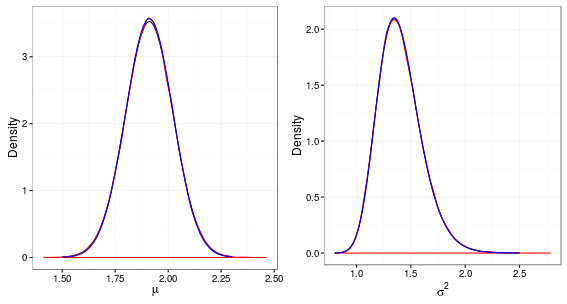
\includegraphics[width=0.7\linewidth,height=\textheight,keepaspectratio]{figures/norminvg}
\caption{Marginal posterior densities for the model described in Section (\ref{subsec:MFVB}). The true density is in red and the MFVB approximation is blue.}
\label{fig:MFVB}
\end{figure}



\subsection{Stochastic Variational Bayes} \label{subsec:SVB}

The requirement for an exponential family model without introducing further approximations, as well as restricting the approximating distribution to the factorisable family may be unsatisfactory in many applications.
\\

\citet{Paisley2012}, \citet{Hoffman2013} and \citet{Ranganath2014} have adapted a gradient ascent algorithm for use in Variational Bayes, which selects the optimal auxiliary parameter vector $\lambda$ for a given functional form of $q_{\lambda}(\theta | y_{1:T})$. This implementation is referred to as Stochastic Variational Bayes (SVB).
\\

For a fixed choice of $q$ SVB maximises the ELBO with respect to $\lambda$ through stochastic gradient ascent, where repeated Monte Carlo estimates of $\partial\mathcal{L}(q, \lambda) / \partial \lambda$, as $\widehat{\partial\mathcal{L}(q, \lambda) / \partial \lambda}$, are calculated. The gradient estimates are used to update $\lambda$ through the simple recursion
\begin{equation}
\label{SVB:gradientAscent}
\lambda^{(m+1)} = \lambda^{(m)} + \rho^{(m)} \widehat{\frac{\partial\mathcal{L}(q, \lambda)}{\partial \lambda}} \bigg\rvert_{\lambda = \lambda^{(m)}}
\end{equation}
until the change from $\mathcal{L}(q, \lambda^{(m)})$ to $\mathcal{L}(q, \lambda^{(m+1)})$ falls below some pre-specified threshold \citep{Hoffman2013}. Intuitively, individual elements of $\lambda$ will increase if the estimate of the slope of $\mathcal{L}(q, \lambda^{(m)})$ is positive at the current point, and will decrease if that estimate is negative, until each element of $\lambda$ reaches a point where the slope is zero. This procedure is guaranteed to converge to a local maximum \citep{Robbins1951} if the sequence $\rho^{(m)}, m = 1, 2 , \ldots$, satisfies
\begin{align}
&\sum_{m=1}^{\infty} \rho^{(m)} =  \infty \\
&\sum_{m=1}^{\infty} (\rho^{(m)})^2 <  \infty.
\end{align}
In this paper the sequence $\rho^{(m)}$ is provided by the Adam algorithm of \citet{Kingma2014b} which is described in the appendix.
\\

Three popular choices for the Monte Carlo estimator of $\partial\mathcal{L}(q, \lambda) / \partial \lambda$ are discussed: the score gradient estimator of \citet{Ranganath2014}, the reparameteterised estimator of \citet{Kingma2014a} and the generalised reparameterised estimator of \citet{Ruiz2016}, described below. Each gradient estimator places different restrictions on the choice of model and approximation, which in general are much less restictive tham MFVB.

\subsubsection{The Score Gradient Estimator}
\label{subsubsec:SVBScore}
The score gradient estimator can be derived by taking the derivative of (\ref{VB:ELBO}) with respect to $\lambda$, 

\begin{align}
\frac{\partial \mathcal{L}(q, \lambda)}{\partial \lambda} &= \frac{\partial}{\partial \lambda}\int q_{\lambda}(\theta | y_{1:T}) \left(\log(p(y_{1:T}, \theta)) - \log(q_{\lambda}(\theta | y_{1:T}))\right) d\theta \nonumber \\
&= \int  \frac{\partial}{\partial \lambda}\bigg[ q_{\lambda}(\theta | y_{1:T}) \left(\log(p(y_{1:T}, \theta)) - \log(q_{\lambda}(\theta | y_{1:T}))\right) \bigg] d\theta \label{SVB:deriv1} \\
&= \int \frac{\partial q_{\lambda}(\theta | y_{1:T})}{\partial \lambda}  \left(\log(p(y_{1:T}, \theta)) - \log(q_{\lambda}(\theta | y_{1:T}))\right) d\theta \nonumber \\
&+ \int q_{\lambda}(\theta | y_{1:T}) \left( \frac{\partial \log(p(y_{1:T}, \theta)) - \log(q_{\lambda}(\theta | y_{1:T}))}{\partial \lambda} \right) d\theta \nonumber \\
&= \int \frac{\partial q_{\lambda}(\theta | y_{1:T})}{\partial \lambda}  \left(\log(p(y_{1:T}, \theta)) - \log(q_{\lambda}(\theta | y_{1:T}))\right) d\theta \nonumber \\
&- \int q_{\lambda}(\theta | y_{1:T})\frac{\partial \log(q_{\lambda}(\theta | y_{1:T}))}{\partial \lambda} d\theta \label{SVB:deriv2}
\end{align}
where (\ref{SVB:deriv1}) follows from the dominated convergence theorem \citep{Casella2002}, noting that the final term in (\ref{SVB:deriv2}) is the expected value of the score of $q_{\lambda}(\theta | y_{1:T}))$, which is equal to zero. 
\\

This result, and the fact that $\partial q_{\lambda}(\theta | y_{1:T}) / \partial \lambda = \left[\partial \log(q_{\lambda}(\theta | y_{1:T})) / \partial \lambda \right] q_{\lambda}(\theta | y_{1:T})$, is substituted into (\ref{SVB:deriv2}),
\begin{align}
\frac{\partial \mathcal{L}(q, \lambda)}{\partial \lambda} &=  \int  q_{\lambda}(\theta | y_{1:T}) \frac{\partial \log(q_{\lambda}(\theta | y_{1:T}))}{\partial \lambda}  \left(\log(p(y_{1:T}, \theta)) - \log(q_{\lambda}(\theta | y_{1:T}))\right) d\theta \nonumber \\
&= \mathbb{E}_{q} \left[ \frac{\partial \log(q_{\lambda}(\theta | y_{1:T}))}{\partial \lambda}  \left(\log(p(y_{1:T}, \theta)) - \log(q_{\lambda}(\theta | y_{1:T}))\right) \right]. \label{SVB:deriv3}
\end{align}

The expectation in (\ref{SVB:deriv3}) is often intractable, so stochastic Monte Carlo estimates of the gradient of the ELBO are instead taken by
\begin{equation}
\label{SVB:scoreDeriv}
\widehat{\frac{\partial\mathcal{L}(q, \lambda)}{\partial \lambda}}_{SC} = \frac{1}{S} \sum_{i = 1}^S \frac{\partial \log(q_{\lambda}(\theta^{(i)} | y_{1:T}))}{\partial \lambda} \left(\log(p(y_{1:T}, \theta^{(i)})) - \log(q_{\lambda}(\theta^{(i)} | y_{1:T})) \right),
\end{equation}
where $\theta^{(i)} \sim q_{\lambda}(\theta | y_{1:T})$.
\\

This estimator often has a very large variance, which can be reduced with control variates \citep{Ross2002}. 
\\

Control variates replace the function being estimated via Monte Carlo simulation with a different function with the same expectation but reduced variance. Referring to the original function in (\ref{SVB:deriv3}) as $g(\theta)$, a new function $h(\theta)$ is defined as
\begin{equation}
\label{SVB:CV1}
h(\theta) = g(\theta) - a(j(\theta) - \mathbb{E}_q(j(\theta))).
\end{equation}
Note that $\mathbb{E}_q(g(\theta)) = \mathbb{E}_q(h(\theta))$, and 
\begin{equation}
\label{SVB:CV2}
\mbox{Var}(h(\theta)) = \mbox{Var}(g(\theta)) + a^2 \mbox{Var}(j(\theta)) - 2 a \mbox{Cov}(g(\theta, j(\theta))).
\end{equation}
Control variates require some function $j(\theta)$ with a known mean and a large positive covariance with $g(\theta)$ so that $\mbox{Var}(h(\theta)) < \mbox{Var}(g(\theta))$ for some choice of $a$.
\\

A possible choice is 
\begin{equation}
\label{SVB:CV3}
j(\theta) = \frac{\partial \log(q_{\lambda}(\theta | y_{1:T}))}{\partial \lambda}
\end{equation}
as this has an expected value of zero, and is already calculated as a by-product of (\ref{SVB:scoreDeriv}).
\\

The final component to consider is the choice of $a$ to minimises $\mbox{Var}(h(\theta))$.  By taking the derivative of (\ref{SVB:CV2}) with respect to $a$ and setting this to zero, the variance minimising value of $a$ is
\begin{equation}
\label{SVB:CV4}
\hat{a} = \frac{\mbox{Cov}(g(\theta), j(\theta))}{\mbox{Var}(j(\theta))}
\end{equation}
which can be estimated from the $S$ Monte Carlo samples. The final score gradient estimator is given by
\begin{equation}
\label{SVB:scoreDeriv2}
\widehat{\frac{\partial\mathcal{L}(q, \lambda)}{\partial \lambda}}_{SC2} = \frac{1}{S} \sum_{i = 1}^S \frac{\partial \log(q_{\lambda}(\theta^{(i)} | y_{1:T}))}{\partial \lambda} \left(\log(p(y_{1:T}, \theta^{(i)})) - \log(q_{\lambda}(\theta^{(i)} | y_{1:T})) - \hat{a} \right).
\end{equation}


\subsubsection{The Reparameterised Gradient Estimator}
\label{subsubsec:SVBRP}
An alternative, lower variance approach (see eg. \cite{Rezende2014}; \cite{Ruiz2016}), is to estimate the gradient of the ELBO by reparameterisation. Reparameterisation introduces an auxiliary variable $\epsilon$ and differentiable transformation $\theta = f(\epsilon, \lambda)$ to rephrase Variational Bayes optimisation as the equivalent search for the set of parameters $\lambda$ for a fixed transformation $f$ that minimises the Kullback Leibler divergence from some distribution $r(\epsilon)$ with zero free parameters to the implied posterior distribution of $\epsilon$,
\begin{equation}
\label{SVB:rpDist}
p(f(\epsilon, \lambda) | y_{1:T}) = p(\theta | y_{1:T}) |J^{-1}(\epsilon, \lambda)|
\end{equation}
where $J(\epsilon, \lambda)$ is the Jacobian Matrix of the transformation $f(\epsilon, \lambda)$. Examples of $f$ and $r(\epsilon)$ include treating $\theta$ as location-scale transformation from a standard normal $r(\epsilon)$, or an inverse-CDF transformation from a uniform$(0, 1)$ $r(\epsilon)$. 
\\

The ELBO can be reparameterised by substituting $p(y_{1:T}, \theta) = p(y_{1:T}, f(\epsilon, \lambda))|J(\epsilon, \lambda)|$ into (\ref{VB:ELBO}),
\begin{equation}
\label{SVB:rpELBO}
\mathcal{L}(q, \lambda) = \mathbb{E}_{r(\epsilon)} \bigg[\log(p(y_{1:T}, f(\epsilon,\lambda))|J(\epsilon, \lambda)|) - \log(r(\epsilon))\bigg].
\end{equation}

The gradient of the reparameterised ELBO with respect to $\lambda$ is given by 
\begin{align}
\label{SVB:rpELBODeriv}
\frac{\partial\mathcal{L}(q, \lambda)}{\partial \lambda} &= \frac{\partial}{\partial \lambda} \bigg( \mathbb{E}_{r(\epsilon)} \bigg[\log\big(p(y_{1:T}, f(\epsilon,\lambda))|J(\epsilon, \lambda)|\big) - \log(r(\epsilon))\bigg] \bigg) \nonumber \\
&= \mathbb{E}_{r(\epsilon)} \left[ \frac{\partial}{\partial \lambda} \bigg(\log(p(y_{1:T}, f(\epsilon,\lambda))) + \log(|J(\epsilon, \lambda)|) - \log(r(\epsilon)) \bigg)\right] \nonumber \\
&= \mathbb{E}_{r(\epsilon)} \left[ \frac{\partial \log(p(y_{1:T}, f(\epsilon,\lambda)))}{\partial f(\epsilon,\lambda)} \frac{\partial f(\epsilon,\lambda)}{\partial \lambda}  + \frac{\partial \log(|J(\epsilon, \lambda)|)}{\partial \lambda} \right].
\end{align}

This form leads to the reparameterised gradient estimator,
\begin{equation}
\label{SVB:rpDeriv}
\widehat{\frac{\partial\mathcal{L}(q, \lambda)}{\partial \lambda}}_{RP} = \frac{1}{S}  \sum_{i = 1}^S \frac{\partial f(\lambda, \epsilon^{(i)})}{\partial \lambda} \frac{\partial \log(p(y_{1:T}, \theta))}{\partial \theta} \bigg\rvert_{\theta = f(\lambda, \epsilon^{(i)})} + \frac{\partial \log(J(\lambda, \epsilon^{(i)}))}{\partial \lambda}, 
\end{equation}
where $\epsilon^{(i)} \sim r(\epsilon)$. 
\\

The approximating distribution $q_{\lambda}(\theta | y_{1:T})$ can then be recovered by applying $\theta = f(\epsilon, \lambda)$ to $r(\epsilon)$,
\begin{equation}
\label{SVB:rpQ}
q_{\lambda}(\theta | y_{1:T}) = r(f(\epsilon, \lambda)) |J(\epsilon, \lambda)| 
\end{equation}

This approach treats $q_{\lambda}(\theta | y_{1:T})$ as the distribution implied by the transformation $f$ of $r(\epsilon)$, restricting the class of approximating families that can be used. 


\subsubsection{The Generalised Reparameterised Gradient Estimator}
\label{subsubsec:SVBGRP}
A third gradient estimator, the generalised reparameterisation estimator of \citet{Ruiz2016} allows $r(\epsilon)$ to depend on the auxiliary vector $\lambda$ so long as the first moment of $r(\epsilon)$ is independent of $\lambda$. 
\\

Reparameteried approximating distributions $q_{\lambda}(\theta | y_{1:T})$ cannot be constructed to belong to common families such as the Gamma, Beta, and Dirichlet distribution. With a careful choice of $r(\epsilon)$ and $f$, these can be constructed via generalised reparameterisation, which retains the benefits of a relatively low variance compared to the score gradient estimator.
\\

Gradient estimates can be obtained by taking Monte Carlo estimates of 
\begin{equation}
\label{SVB:grp}
\frac{\partial\mathcal{L}(q, \lambda)}{\partial \lambda} = \textbf{g}^{rep} + \textbf{g}^{corr} - \frac{\partial}{\partial \lambda} \mathbb{E}_{q} \left[ \log(q_{\lambda}(\theta | y_{1:T})) \right]
\end{equation}
where
\begin{align}
\textbf{g}^{rep} =  \mathbb{E}_{q} &\left[\frac{\partial \log(p(y_{1:T}, \theta))}{\partial \theta} \frac{\partial f^{-1}(\theta, \lambda)}{\partial \lambda} \right] \\
\textbf{g}^{corr} =  \mathbb{E}_{q} &\left[ \log(p(y_{1:T}, \theta)) \left( \frac{\partial \log(q_{\lambda}(\theta | y_{1:T}))}{\partial \theta} \frac{\partial f^{-1}(\theta, \lambda)}{\partial \lambda}  \right. \right. \nonumber \\
&+ \left. \left. \frac{\partial \log(q_{\lambda}(\theta | y_{1:T}))}{\partial \lambda} + \frac{\partial |J^{\prime}(\theta, \lambda)|}{\partial \lambda} \right) \right]
\end{align}
where $f^{-1}(\theta, \lambda)$ is the inverse of $f(\epsilon, \lambda)$, evaluated at $\theta$, and $J^{\prime}(\theta, \lambda)$ is the Jacobian matrix of $f^{-1}(\theta, \lambda)$.
\\

If $f$ is the identity function, $\textbf{g}^{rep} = 0$ and the score gradient estimator is recovered. Alternatively if $r(\epsilon)$ does not depend on $\lambda$, $\textbf{g}^{corr} = 0$ and the reparameterised gradient estimator is recovered.
\\

An outline of SVB is provided in Algorithm \ref{alg:SVB}.
\\

\begin{algorithm}[H]
 \SetKwInOut{Input}{Input}
 \Input{Approximation family $q$ or auxiliary distribution $r$ and function $f$}
 \KwResult{Variational Approximation}
 Set $m = 1$\;
 Initialise $\lambda^{(1)}$ randomly\;
 Evaluate $\mathcal{L}(q, \lambda^{(1)})$ with the Monte Carlo estimator (\ref{VB:ELBO-MC}) using $\lambda^{(1)}$\;
 \While{$|\mathcal{L}(q, \lambda^{(m)} - \mathcal{L}(q, \lambda^{(m-1)})| > \epsilon$}{
  Set $m = m + 1$\;
  Simulate $\theta^{(i)}$ for $i = 1, \ldots S$ from $q_{\lambda}(\theta | y_{1:T})$\;
  Estimate $\widehat{\frac{\partial\mathcal{L}(q, \lambda)}{\partial \lambda}}$ via (\ref{SVB:scoreDeriv2})\;
  OR\;
  Simulate $\epsilon^{(i)}$ for $i = 1, \ldots S$ from $r(\epsilon)$\;
  Estimate $\widehat{\frac{\partial\mathcal{L}(q, \lambda)}{\partial \lambda}}$ via (\ref{SVB:rpDeriv})\;
  OR\;
  Simulate $\theta^{(j)}$ for $i = 1, \ldots S$ from $q_{\lambda}(\theta | y_{1:T})$\;
   Estimate $\widehat{\frac{\partial\mathcal{L}(q, \lambda)}{\partial \lambda}}$ via (\ref{SVB:grp})\;
  Apply Update $\lambda^{(m)} = \lambda^{(m-1)} + \rho^{(m-1)} \widehat{\frac{\partial\mathcal{L}(q, \lambda)}{\partial \lambda}}$\;
  Evaluate $\mathcal{L}(q, \lambda^{(m)})$\;
 }
 \caption{Stochastic Gradient Ascent for Variational Bayes}
  \label{alg:SVB}
\end{algorithm}

\subsubsection{Randomised Quasi Monte Carlo}
\label{subsubsec:SVBRQMC}

Choosing the number of samples per estimate, $S$, involves a trade-off between the computation time per gradient estimate and the stochastic noise present in each estimate. An increased value of $S$ will the Monte Carlo error, and generally reduce the number of iterations required for the ELBO to converge, at a linear increase in computation time per iteration.
\\

To reduce the Monte Carlo error, following \citet{Gunawan2017} Randomised Quasi Monte Carlo (RQMC) is used instead, which has shown to be more efficient than standard Monte Carlo in many applications, including Variational Bayes (see \cite{Niederreiter1992, Caflisch1998}, and \cite{Buchholz2018}). In RQMC, a deterministic sequence of numbers in the $k-$dimensional unit hypercube $[0, 1)^k$, where $k$ is the dimension of $\theta$ are generated. This sequence designed to have a low star discrepancy, so that the proportion of points in any $k-$dimensional subspace of $[0, 1)^k$ is close to the volume of that subspace.
\\

These are randomised each iteration to preserve the low discrepency properties while inducing a central limit theorem so that the gradient estimate is unbiased. See \citet{Matousek1998} for more details.
\\

Selecting $S$ of the resulting coordinates in the unit hypercube, and transforming these using the inverse-CDF of either $q_{\lambda}(\theta | z)$ or $r(\epsilon)$ simulates $S$ draws that can be used in any of the discussed gradient estimators.

\subsubsection{Time Series Example}
\label{subsubsec:SVBTS}

Some of the major advantages of SVB relative to MFVB are its flexibility to be applied to non exponential family models, and the ability to include parameter dependence in the approximating distribution. To illustrate this, consider the second order auto-regressive time series model, denoted by AR(2), and described by 
\begin{equation}
\label{SVBTS:AR2}
y_t = \phi_1 y_{t-1} + \phi_2 y_{t-2} + \epsilon_t
\end{equation}
where $\epsilon_t \sim \mathcal{N}(0, \sigma^2)$ for $t = 3, 4 \ldots, T$. The first two observations, $y_1$ and $y_2$ are distributed according to 
\begin{equation}
\label{SVBTS:Initial}
y_1, y_2, \sim \mathcal{N}(\boldsymbol{0}, \Sigma)
\end{equation}
where 
\begin{align}
\Sigma &= \left[ \begin{array}{cc} \gamma(0) & \gamma(1) \\ \gamma(1) & \gamma(0) \end{array} \right], \nonumber \\
\gamma(0) &= \sigma^2 \frac{1-\phi_2}{(1+\phi_2)((1-\phi_2)^2 - \phi_1^2)} \nonumber, \\
\gamma(1) &= \sigma^2 \frac{\phi_1}{(1+\phi_2)((1-\phi_2)^2 - \phi_1^2)} \nonumber.
\end{align}

The following prior distribution is chosen
\begin{equation}
p(\sigma^2, \phi_1, \phi_2) \propto \sigma^{-2} \mathbb{I}(\phi_2 > -1)\mathbb{I}(\phi_2 < 1 + \phi_1) \mathbb{I}(\phi_2 < 1 - \phi_1), 
\label{SVBTS:Prior}
\end{equation}
where $\mathbb{I}$ is the indicator function that equals one if the condition in the brackets is true and zero otherwise. This prior has uniform positive mass for the pair $(\phi_1, \phi_2)$ across the AR(2) stationary region, and zero mass outside of this region. Note that this prior is not conjugate due to the form of $\phi_1$ and $\phi_2$ in $\Sigma$, and thus MFVB cannot be applied. 

Data was simulated with $T = 150, \sigma^2 = 1, \phi_1 = 0.7$ and $\phi_2 = 0.2$, then both RWMH-MCMC and SVB are applied. $q_{\lambda}(\theta | y_{1:T})$ is chosen to be the product of a bivariate normal distribution for $\phi_1$ and $\phi_2$, and an Inverse Gamma distribution for $\sigma^2$.

Figure \ref{fig:SVB} displays the marginal and bivariate posterior distributions that result from each of the Stochastic Variational Bayes (blue) and the MCMC (red) approaches. In the case of MCMC, a kernel estimate obtained from the relevant posterior sample is displayed. As is clear from the figure, SVB appears to have selected values for $\lambda$ that closely match the MCMC posterior distribution. SVB required approximately one hundredth of the computation time required for MCMC.

\begin{figure}[htbp]
\centering
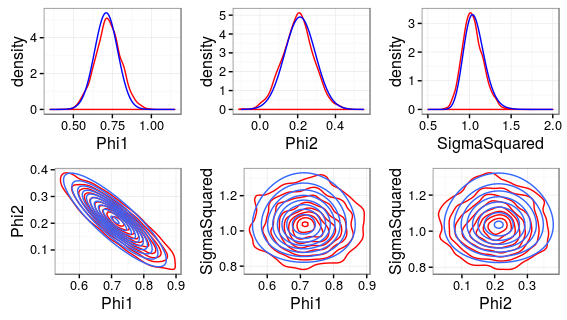
\includegraphics[width=0.7\linewidth,height=\textheight,keepaspectratio]{figures/VBfit.png}
\caption{The fit of an SVB algorithm (blue) compared to MCMC (red) for the AR(2) model.}
\label{fig:SVB}
\end{figure}

\subsection{Stein Variational Gradient Descent}
\label{subsec:Stein}

\cite{Liu2016} introduce Stein Variational Gradient Descent, which creates a KL-divergence minimising particle approximation of the form
\begin{equation}
\label{Stein:Approx}
q_m(\theta | y_{1:T}) = \frac{1}{N}\sum_{i=1}^N \delta(\theta^{(i)}_l).
\end{equation} 
They approach this by proposing a sequence of approximating distributions, starting with particles $\theta^{(i)}_0$ drawn from some arbitrary $q_{0}(\theta)$, then transformed to $\theta^{(i)}_{m+1}$ via
\begin{equation}
\label{Stein:Transform}
\theta^{(i)}_{m+1} = \theta^{(i)}_ml + \epsilon_m \phi_m(\theta^{(i)}_m)
\end{equation}
where $\epsilon_m$ is some small constant and $\phi_m(\cdot)$ is some continuously differentiable function. The sequence $\phi_1, \phi_2, \ldots, \phi_m$ could be considered the parameters of the reparametersied VB function $\theta_m = f(\theta_0, \lambda)$.
\\

\cite{Liu2016} proves that, for a fixed choice $\phi_m$, 
\begin{equation}
\label{Stein:Derivative}
\frac{\partial KL[q_m(\theta | y_{1:T}) \hspace{1mm} || \hspace{1mm} p(\theta | y_{1:T})]}{\partial \epsilon} \bigg \vert_{\epsilon = 0} = - \mathbb{E}_{q_m} \left[ \mbox{trace}(A_p \phi_l(\theta)) \right]
\end{equation}
where $A_p$ is the Stein operator
\begin{equation}
\label{Stein:Operator}
A_p \phi(\theta) = \frac{\partial \log(p(y_{1:T}, \theta))}{\partial \theta} \phi(\theta)^{\prime} + \frac{\partial \phi(\theta)}{\partial \theta}.
\end{equation}

The aim of Stein Variational Gradient Descent is to choose the sequence of functions $\phi_m(\cdot)$ that minimises $KL[q_m(\theta | y_{1:T}) \hspace{1mm} || \hspace{1mm} p(\theta | y_{1:T})]$ with the least number of iterations, so at each iteration $m$ we want to choose the function $\phi_m(\cdot)$ that minimises the gradient of the KL divergence (remember this is a minimisation problem!).
\\

Restricting $\phi_m$ to the set of functions in the reproducing kernel Hilbert space $\mathcal{H}$ for some positive definite kernel $k(\cdot, \cdot)$ for which $||\phi||_{\mathcal{H}} \leq 1$, it can be shown that
\begin{equation}
\label{Stein:optPhi}
\hat{\phi}_m(\cdot) = \arg \underset{\phi}{\max} \hspace{1mm} \mathbb{E}_{q_m} \left[ \mbox{trace}(A_p \phi_m(\theta)) \right] = \mathbb{E}_{q_m} \left[ A_p k(\theta, \cdot) \right].
\end{equation}

Noting that the expectation in (\ref{Stein:optPhi}) is over a discrete distribution, the function evaluation $\hat{phi}_m(\theta^{(i)})$ is calculated as
\begin{equation}
\label{Stein:estPhi}
\hat{\phi}_m(\theta^{(i)}) = \frac{1}{N} \sum_{j=1}^N \left[ k(\theta_m^{(j)}, \theta_m^{(i)}) \frac{\partial \log(p(y_{1:T}, \theta))}{\partial \theta} \bigg \vert_{\theta = \theta^{(j)}_m} + \frac{\partial k(\theta, \theta^{(i)})}{\partial \theta} \bigg \vert_{\theta = \theta^{(j)}_m} \right]
\end{equation}
where $N$ is the number of particles. The particles are then transformed according to (\ref{Stein:Transform}) for as many iterations as desired.
\\

The sum in (\ref{Stein:estPhi}) may be carried out over only a subset of the particles to reduce computation time. In this case, the gradient is replaced with a stochastic estimate and the sequence $\epsilon_m$ must follow the Robbins-Monro conditions.
\\

\cite{Liu2017} goes on to show that, in the limit as $m \rightarrow \infty$ and $N \rightarrow \infty$, $q_m(\theta | y_{1:T})$ converges to $p(\theta | y_{1:T})$ 


\section{Updating Bayesian Inference}
\label{sec:UpdateBayes}

The discussion is extended to settings where data is regularly being observed in an online setting, resulting in a sequence of time points $T_1, T_2, \ldots$, from which a sequence of posterior distributions $p(\theta | y_{1:T_1}), p(\theta | y_{1:T_2}), \ldots$, may be desired.
\\

This is illustrated in Figure \ref{fig:updatetimeUpdate} for data taken from vehicle in the Next Generation Simulation (NGSIM) dataset provided by the US Federal Highway Administration (FHWA), travelling towards the right. In the left panel, the vehicle has been observed for a time period $T_{n}$ resulting in data $y_{1:T_{n}}$ which can be incorporated into the posterior distribution $p(\theta | y_{1:T_{n}})$. In the right panel, after observation for an additional period to time $T_{n+1}$, an additional $T_{n+1} - T_{n}$ data points are available, and posterior inference could be improved by incorporating the information contained in $y_{T_{n}+1:T_{n+1}}$ to form the posterior approximation $p(\theta | y_{1:T_{n+1}})$.

\begin{figure}[htbp]
\centering
\includegraphics[width = 0.95\textwidth, height = 0.15\textheight]{figures/carUpdate}
\caption{Left: The path of a vehicle in the NGSIM dataset that has been observed for a time period equal to $T_{n}$, where the direction of travel is from the left to the right. Right: The same vehicle at a later time $T_{n+1}$, with the extra $T_{n+1} - T_{n}$ observations denoted by the dashed line. Posterior inference about this vehicle could be updated from time $T_{1}$ to time $T_{2}$ by the inclusion of this additional information.}
\label{fig:updatetimeUpdate}
\end{figure}

From Bayes Rule, the posterior distribution at time $T_{n+1}$, $p(\theta | y_{1:T_{n+1}})$ is given by
\begin{equation}
\label{update:truePost}
p(\theta | y_{1:T_{n+1}}) \propto p(y_{1:T_{n_1}} | \theta)p(\theta).
\end{equation}
where the likelihood is given by
\begin{equation}
\label{update:likelihood}
p(y_{1:T_n} | \theta) = p(y_1) \prod_{t=2}^{T_n} p(y_t | \theta, y_{1:t-1}).
\end{equation}
the product of $T_n$ terms. If the posterior at time $T_{n}$ is available, the likelihood can be reduced to a product of only $T_{n+1} - T_{n}$ terms by applying Bayes' Rule,
\begin{equation}
\label{update:updatePost}
p(\theta | y_{1:T_{n+1}}) \propto p(y_{T_{n}+1:T_{n+1}} | \theta, y_{1:T_{n}})p(\theta | y_{1:T_{n}}),
\end{equation}
However, many Bayesian computational methods require the evaluation of $p(\theta | y_{1:T_{n}})$ at arbitrary values of $\theta$, which is computationally infeasible for many posterior distributions of interest and so the more intensive (\ref{update:truePost}) is typically applied instead.

\subsection{Sequential Monte Carlo}
\label{subsec:SMC}

Sequential Monte Carlo (SMC, \cite{Doucet2000}, \cite{Arulampalam2002}) algorithms, often referred to as Particle Filters , are a technique to update a set of samples distributed according to $p(\theta | y_{1:T_n})$ to the distribution $p(\theta | y_{1:T_{n+1}})$. SMC approaches work via a repeated application of an importance sampler with respect to a common set of samples, or particles, drawn from the candidate distribution $r(\theta)$.
\\

After applying importance sampling, a discrete approximation to the posterior can be provided by
\begin{equation}
\label{SMC:Approx}
p^*(\theta | y_{1:T_n}) = \sum_{i=1}^S w^{(i)}_{T_n} \delta(\theta^{(i)})
\end{equation}
where $\delta$ is the Dirac delta function and $w^{(i)}_{T_n}$ are the $S$ importance sampler weights up to time $T_n$.
\\

While the critical choice of the initial $r(\theta)$ is left to the user, SMC concerns itself with the recursive application of importance sampling where the candidate distribution at some time $T_{n+1}$ is given by the previous set of particles and weights that compose (\ref{SMC:Approx}). In this case, the SMC update to 
\begin{equation}
\label{SMC:Update}
p^*(\theta | y_{1:T_{n+1}}) = \sum_{i=1}^S w^{(i)}_{T_{n+1}} \delta(\theta^{(i)})
\end{equation}
is performed by updating the unnormalised weights,
\begin{align}
\hat{w}^{(i)}_{T_{n+1}} &= \frac{p(y_{1:T_{n+1}}, \theta^{(i)})}{r(\theta^{(i)})} \nonumber \\
&= \frac{p(y_{T_{n}+1:T_{n+1}} | \theta^{(i)}) p(y_{1:T_n}, \theta^{(i)})}{r(\theta^{(i)})} \nonumber \\
&= p(y_{T_{n}+1:T_{n+1}}| \theta^{(i)}) \hat{w}^{(i)}_{T_n}, \label{SMC:UpdateWeights},
\end{align}
which are normalised by
\begin{equation}
\label{SMC:UpdateWeightsNorm}
w^{(i)}_{T_{n+1}} = \frac{\hat{w}^{(i)}_{T_{n+1}}}{\sum_{i=1}^S \hat{w}^{(i)}_{T_{n+1}}}.
\end{equation}

Repeated SMC updates often exhibit weight degeneration, where the values of each $w^{(i)}_{T_{n+1}}$ except one approaches zero, reducing the effective sample size of the approximation.
\iffalse

 which is estimated by
\begin{equation}
\label{SMC:EFF}
\hat{N}_{eff} = \frac{1}{\sum_{i=1}^N (w^{(i)}_{T_{n+1}})^2}.
\end{equation}

A common strategy to avoid this is through resampling, where if after an SMC update $\hat{N}_{eff}$ falls below some threshold, a new set of particles is sampled according to the distribution
\begin{equation}
\label{SMC:Resample}
\theta^{(i)}_{RS} \sim \sum_{i=1}^M w^{(i)}_{T_{n+1}} \delta(\theta^{(i)}).
\end{equation}
After resampling, the weights are each reset to $w^{(i)}_{T_{n+1}} = 1/N$. 
\\

Resampling resets the weights of each particle, however there is a high probability that there will be repeated values in the new set of particles and diversity is reduced.

\textit{After writing this I realise that re-sampling doesn't do anything in non-state-space-models as we don't have a transition equation to refresh the particle diversity. Instead of losing out because most of our particle weights are zero, we're losing out because we're repeating calculations for the same $\theta$ value! This is useful for UVB Importance Sampling, as we will get new proposal distributions to refresh out particle weights.}

\fi

\subsection{Bayesian Filtering? PMMH? Only if we use them later}

\subsection{Online Mean Field Variational Bayes}
\label{subsec:OnlineMFVB}

Mean Field Variational Bayes applied conjugate-exponential family model results in a set of mean field equations that can be written in the form of 
\begin{equation}
\lambda = f(\beta, y_{1:T}) \label{OnlineMFVB:OfflineEq}
\end{equation}
where $\beta$ denotes the prior hyperparameters. 
\\

Let $\lambda_1$ denote the MFVB optimal auxiliary parameters of $q_{\lambda_1}(\theta | y_{1:T_1})$, an approximating distribution chosen to minimise the KL divergence to the posterior after observation of $y_{1:T_1}$, obtained via the application of (\ref{OnlineMFVB:OfflineEq}),
\begin{equation}
\lambda_1 = f(\beta, y_{1:T_1}) \label{OnlineMFVB:OnlineEq1}
\end{equation}

The online MFVB approach first advocated by \cite{Ghahramani2000b} is to treat $\lambda_n$ as an updated form of the prior hyperparameters and re-apply the meanfield equations as
\begin{align}
\lambda_{n+1} = f(\lambda_n, y_{T_n+1:T_{n+1}}) \label{OnlineMFVB:OnlineEq2}
\end{align}

This results in a sequence of MFVB distributions $q_{\lambda_1}(\theta | y_{1:T_1}), q_{\lambda_2}(\theta | y_{1:T_2}), \ldots$ to approximate each of the sequence of posteriors $p(\theta | y_{1:T_1}), p(\theta | y_{1:T_2}), \ldots$.
\\ 

See \cite{Smidl2004}, \cite{Hoffman2010}, \cite{Wang2011}, \cite{Broderick2013}, and \cite{Kabisa2016} for examples of applications of Online MFVB.

\subsection{Online Stochastic Variational Bayes}
\label{subsec:OnlineSVB}

The stochastic gradient ascent approach utilised by SVB, where $\partial\mathcal{L}(q, \lambda) / \partial \lambda$ is estimated by $\widehat{\partial\mathcal{L}(q, \lambda) / \partial \lambda}$, will converge to a local maximum for any unbiased gradient estimator (\cite{Robbins1951}, \cite{Bottou1999}, \cite{Bottou2008}).
\\

Online SVB does not provide an approximate distribution at each of a sequence of time points $T_1, T_2, \ldots$, but allows for SVB inference to be substantially sped up by calculating the likelihood of only a subset of the entire dataset each iteration (\cite{Hoffman2013}, \cite{Titsias2014}).
\\

If the data $y_{1:T}$ is conditionally independent given $\theta$, the log-likelihood decomposes into the sum
\begin{equation}
\label{OnlineSVB:likelihood}
\log(p(y_{1:T} | \theta)) = \sum_{t=1}^T \log(p(y_t | \theta)).
\end{equation}

By subsetting $y_{1:T}$ into length $N$ `minibatches', where $N < T$, Online SVB replaces the log-likelihood in the gradient estimates with an unbiased estimator
\begin{equation}
\label{OnlineSVB:likelihoodEstim}
\widehat{\log(p(y_{1:T} | \theta))} = \frac{T}{N} \sum_{t=1}^N \log(p(y_t | \theta))
\end{equation}
where the sum in (\ref{OnlineSVB:likelihoodEstim}) is only over components of $y_{1:T}$ that are in the current minibatch. As this is unbiased, the gradients $\widehat{\partial\mathcal{L}(q, \lambda) / \partial \lambda}$ retain their unbiased properties.
\\

Each iteration of the gradient ascent algorithm should use a different subset of the data, so that sequential iterations cycle through the entire dataset. 
\\

\chapter{Approximate Bayesian Updating}
\label{chap:UVB}

This chapter introduces Updating Variational Bayes (UVB), a mechanism where an SVB approximation can be updated from $q_{\lambda_n}(\theta | y_{1:T_n})$ to  $q_{\lambda_{n+1}}(\theta | y_{1:T_{n+1}})$ using only the additional data $y_{T_{n}+1:T_{n+1}}$, and where the computation required by the update does not increase with $n$. Note that the $n$ and $n+1$ subscripts on $\lambda$ are introduced to differentiate the auxiliary parameter vector conditioned on data up to times $T_{n}$ and $T_{n+1}$.
\\

An importance sampling extension to UVB is introduced, which allows for further computational cost reductions in scenarios where the marginal information in $y_{T_n+1:T_{n+1}}$ is relatively small.
\\

The application of UVB to Bayesian Filtering, the recursive problem of inferring the distribution of some unobserved latent states $x_{1:T_n}$ given observations of data $y_{1:T_n}$ as $n$ increases, is discussed. 
\\

An additional importance sampling framework which can be used as an error correction mechanism is provided to reduce the impact of using a variational approximation to the posterior. 
\\

Finally several sets of simulated data are analysed to compare the approximation error and runtime for SVB, UVB, and the importance sampled corrections.

\section{Updating Variational Bayes}
\label{sec:UVB}

Bayesian updating refers to the repeated use of the posterior update equation first introduced in Section \ref{sec:UpdateBayes},
\begin{equation}
\label{UVB:updatePost}
p(\theta | y_{1:T_{n+1}}) \propto p(y_{T_{n}+1:T_{n+1}} | \theta, y_{1:T_{n}})p(\theta | y_{1:T_{n}}).
\end{equation}
Note that, in the general case, the right hand side of this proportionality is computationally intractable due to the presence $p(\theta | y_{1:T_n})$.
\\

The application of SVB at time $T_1$ results in the analytically tractable posterior distribution
\begin{equation}
\label{UVB:Time1}
q_{\lambda_1}(\theta | y_{1:T_1}) = \arg \underset{q}{\min} \hspace{1mm} KL[q_{\lambda_1} (\theta | y_{1:T_1}) \hspace{.1cm}||\hspace{.1cm}p(\theta | y_{1:T_1})].
\end{equation}
Starting with this approximation, UVB involved the recursive use of the distribution \\ $q_{\lambda_n}(\theta | y_{1:T_n})$ at time $T_n$ as a substitute for the true posterior in the Bayesian update (\ref{UVB:updatePost}) to form an alternative pseudo-posterior update,
\begin{equation}
\label{UVB:pHatPosterior}
\hat{p}(\theta |  y_{1:T_{n+1}}) \propto p(y_{T_{n}+1:T_{n+1}} | \theta)q_{\lambda_{n}}(\theta | y_{1:T_{n}}).
\end{equation}
As the right hand side of this update is analytically tractable, standard ELBO gradient optimisation methods discussed in Section \ref{subsec:SVB} may be applied to find  
\begin{equation}
\label{UVB:TimeNp1}
q_{\lambda_{n+1}}(\theta | y_{1:T_{n+1}}) = \arg \underset{q}{\min} \hspace{1mm} KL[q_{\lambda_{n+1}} (\theta | y_{1:T_{n+1}}) \hspace{.1cm}||\hspace{.1cm}\hat{p}(\theta | y_{1:T_{n+1}})].
\end{equation}
Minimising the KL divergence in this way is not equivalent to standard VB which minimises $KL[q_{\lambda_{n+1}} (\theta | y_{1:T_{n+1}}) \hspace{.1cm}||\hspace{.1cm}p(\theta | y_{1:T_{n+1}})]$ unless $q_{\lambda_{n}}(\theta |  y_{1:T_{n}}) = p(\theta |  y_{1:T_{n}})$ almost everywhere. This is only possible if the posterior is a member of the family $q$. When this is not the case UVB introduces an additional approximation error to Variational Bayes inference which depends largely on the ability of the family $q$ chosen to adequately approximate the true posterior distribution.
\\

If the updates are equally spaced such that $T_{n+1} - T_{n} = H$ for all $n$, then the computational complexity of UVB as $n$ increases is constant at $O(H)$. In contrast, the computational complexity of SVB is $O(T_{n})$ as it evalutates the posterior via (\ref{update:truePost}) which requires evaluation of the complete data likelihood, $p(y_{1:T_{n}} | \theta)$, at each $T_{n}$.
\\

Choosing the form of the approximating distribution to match the prior distribution allows UVB to be easily implemented, as the prior hyper-parameters are simply replaced with the optimised $\lambda_n$ values after each update.
\\

A summary of the UVB algorithm is given by Algorithm \ref{alg:UVB}.
\\

\begin{algorithm}[H]
 \SetKwInOut{Input}{Input}
 \Input{Prior, Likelihood.}
 \KwResult{Approximating distribution at $T_N$.}
 Observe $y_{1:T_1}$\;
 Use (\ref{SVB:scoreDeriv2}), (\ref{SVB:rpDeriv}), or (\ref{SVB:grp}) to choose the $\lambda_1$ that minimises the KL divergence from $q_{\lambda_1}(\theta | y_{1:T_1})$ to $p(\theta | y_{1:T_1})$ \;
 \For{$n \mbox{ in } 1, \ldots, N-1$}{
   Observe next data $y_{T_{n}+1:T_{n+1}}$\;
   Use $q_{\lambda_{n}}(\theta | y_{1:T_{n}})$ and (\ref{SVB:scoreDeriv2}), (\ref{SVB:rpDeriv}), or (\ref{SVB:grp}) to choose the $\lambda_{n+1}$ that minimises the KL divergence from $q_{\lambda_{n+1}}(\theta | y_{1:T_{n+1}})$ to $\hat{p}(\theta | y_{1:T_{n+1}})$ 
  }
 \caption{Updating Variational Bayes}
  \label{alg:UVB}
\end{algorithm}

\section{Variational Bayesian Filtering} \label{sec:UVBVBF}

\textit{We don't use latent states in any of the models so far so this section isn't used.}

Many models of interest can be expressed as a dynamic state-space, with
\begin{align}
y_t &\sim p(y_t | x_{t}, \theta) \label{VBF:measure} \\
x_t &\sim p(x_t | x_{t-1}, \theta) \label{VBF:transition} ,
\end{align}
where inference of $p(x_t, \theta | y_{1:t})$ is desired at each $t$. This problem is known as \textit{Bayesian filtering}, where the posterior distribution is recursively updated from $p(x_{t-1}, \theta | y_{1:t-1})$ to $p(x_t, \theta | y_{1:t})$ by
\begin{align}
p(x_t, \theta | y_{1:t-1}) &= \int p(x_t | x_{t-1}, \theta) p(x_{t-1}, \theta | y_{1:t-1})x_{t-1} \label{VBF:marginalise} \\
p(x_t, \theta | y_{1:t}) &\propto p(y_t | x_t, \theta) p(x_t, \theta | y_{1:t-1}) \label{VBF:update}
\end{align}
for a given prior distribution $p(x_0, \theta)$. 
\\

For a limited class of models the marginalisation over $x_{t-1}$ in (\ref{VBF:marginalise}) and posterior in (\ref{VBF:update}) are both analytically tractable for all $t$, such as when both (\ref{VBF:measure}) and (\ref{VBF:transition}) are linear and Gaussian. Typically this is not the case and an approximation is required, such as the extended Kalman filter \citep{Anderson1979}, the unscented Kalman filter \citep{Wan2000}, or particle filters (\cite{Doucet2000}, \cite{Arulampalam2002}). Variational Particle Filtering is introduced by \citet{Smidl2008}, in cases where a subset $x_{1, t}$ of $x_t = \{x_{1, t}, x_{2, t}\}$ can be analytically marginalised, and does not discuss simultaneous inference of the static variables $\theta$ which is allowed with UVB below.
\\

Replacing $p(x_{t-1}, \theta | y_{1:t-1})$ with the Variational Bayes approximation \newline $q(x_{t-1} | y_{1:t-1}, \theta)q(\theta|y_{1:t-1})$ the following distributions are obtained 
\begin{align}
\hat{p}(x_t, \theta | y_{1:t-1}) &= q(\theta | y_{1:t-1}) \int p(x_t | x_{t-1}, \theta) q(x_{t-1} | y_{1:t-1}, \theta)x_{t-1} \label{VBF:marginaliseHat} \\
\hat{p}(x_t, \theta | y_{1:t}) &\propto p(y_t | x_t, \theta)\hat{p}(x_t, \theta | y_{1:t-1}). \label{VBF:updateHat}
\end{align}

If (\ref{VBF:transition}) is linear and Gaussian, and  $q(x_{t-1} | y_{1:t-1}, \theta)$ is Gaussian, (\ref{VBF:marginaliseHat}) can be marginalised analytically, allowing the Variational Bayes approximation at time $t$ as
\begin{equation}
\label{VBF:UVBfilter}
\hat{p}(x_t, \theta | y_{1:t}) \approx q(x_{t} | y_{1:t}, \theta)q(\theta|y_{1:t}).
\end{equation}
\\

\section{Correcting Approximation Error} \label{sec:UVBCorrection}

The increasing approximation error introduced by UVB could be offset by an importance sampling correction at each $T_n$. By using the UVB distribution $q_{\lambda_n}(\theta | y_{1:T_n})$ as the proposal $r(\theta)$, the following discrete approximation may be constructed
\begin{equation}
\label{UVBIS:Approx}
p^*(\theta | y_{1:T_n}) = \sum_{i=1}^M w^{(i)}_{T_n} \delta(\theta^{(i)})
\end{equation}
with weights given by
\begin{align}
\hat{w}^{(i)}_{T_n} &= \frac{p(y_{1:T_n} | \theta^{(i)}) p(\theta^{(i)}))}{q(\theta^{(i)} | y_{1:T_n})} \label{UVBIS:Weights} \\
w^{(i)}_{T_n} &= \frac{\hat{w}^{(i)}_{T_n}}{\sum_{i=1}^M \hat{w}^{(i)}_{T_n}} \label{UVBIS:WeightsNorm}
\end{align}
\\

\citet{Yao2018} note that, due to the variational approximation underestimating the tails of the exact posterior, importance sampling in this way often performs poorly with the weights dominated by a few samples. A Pareto-Smoothed importance sampler is suggested as an alternative.

If additional observations $y_{T_n+1}, y_{T_n + 2}, \ldots, y_{T_{n+1}}$, are observed before the update to \\ $q_{\lambda_{n+1}}(\theta | y_{1:T_{n+1}})$ is available, the SMC recursion can be used to update the weights via
\begin{align}
\hat{w}^{(i)}_{T_n+h} &= p(y_{T_n+h} | \theta^{(i)}) \hat{w}^{(i)}_{T_n+h-1}, \label{UVBIS:UpdateWeights} \\
w^{(i)}_{T_n+h} &= \frac{\hat{w}^{(i)}_{T_n+h}}{\sum_{i=1}^M \hat{w}^{(i)}_{T_n+h}}. \label{UVBIS:UpdateWeightsNorm}
\end{align}
for $h = 1, 2, \ldots, T_{n+1} - T_{n}$
\\

Once computation of $q_{\lambda_{n+1}}(\theta | y_{1:T_{n+1}})$ has finished, a fresh set of particles can be sampled from this distribution and significant weight degeneration may be avoided.

\section{Importance Sampled UVB} 
\label{sec:UVBIS}

UVB has significant computational cost savings as it reduces the likelihood from a product of $T_{n+1}$ terms to a product of only $T_{n+1} - T_n$ terms. \\

The gradient ascent algorithm utilised by UVB to fit $q_{\lambda_{n+1}}(\theta | y_{1:T_{n+1}})$ maximises the ELBO by repeated application of the following steps:
\begin{enumerate}
\item At iteration $m$ draw $\theta^{(1)}, \theta^{(2)}, \ldots, \theta^{(S)}$ from $q_{\lambda_{n+1}^{(m)}}(\theta | y_{1:T_{n+1}})$ \\
(alternatively draw $\epsilon^{(1)}, \epsilon^{(2)}, \ldots, \epsilon^{(S)}$ from $r(\epsilon)$ and transform with $\theta = f(\epsilon, \lambda^{(m)}_{n+1})$),
\item Calculate $p(y_{T_{n}+1:T_{n+1}} | \theta)$ for each $\theta = \theta^{(1)}, \theta^{(2)}, \ldots, \theta^{(S)}$ as part of the gradient estimate $\widehat{\frac{\partial\mathcal{L}(q, \lambda_{n+1})}{\partial \lambda_{n+1}}}$,
\item Update $\lambda_{n+1}^{(m+1)} = \lambda_{n+1}^{(m)} + \rho^{(m)}\widehat{\frac{\partial\mathcal{L}(q, \lambda_{n+1})}{\partial \lambda_{n+1}}} \bigg\rvert_{\lambda_{n+1} = \lambda^{(m)}_{n+1}}$,
\item Set $m = m + 1$.
\end{enumerate}
After each iteration, $\lambda_{n+1}$ changes, and hence $\theta$ must be resamples at step one, and the likelihood must be recalculated with these new samples. 
\\

\citet{Sakaya2017} note that calulation of the data likelihood is the most computationally expensive component of the gradient estimate. They propose that the $\theta$ samples used at some iteration $m$ could be re-used for iterations $m + 1, m + 2, \ldots m + h$ to calculate the gradient as an importance sampled estimate. 
\\

As $\theta$ is constant between iterations, the likelihood does not need to be recalculated and optmisation is sped up. For some $h$ the difference between $q_{\lambda_{n+1}^{(m)}}(\theta | y_{1:T_{n+1}})$ and $q_{\lambda_{n+1}^{(m+h)}}(\theta | y_{1:T_{n+1}})$ becomes large, reducing the effective sample size of the importance sampler weights and degrading the gradient estimate. At this stage \citet{Sakaya2017} resample $\theta$ and recalculate the likelihoods.
\\

This idea is readily extendable to the UVB context to derive an importance sampled UVB (IS-UVB) gradient estimator.
\\

Recall the score ELBO gradient for UVB,
\begin{equation}
\label{UVBIS:scoreGrad}
\frac{\partial\mathcal{L}(q, \lambda_{n+1})}{\partial \lambda_{n+1}} = \int_{\theta} q_{\lambda_{n+1}}(\theta | y_{1:T_{n+1}}) \frac{\partial \log(q_{\lambda_{n+1}}(\theta | y_{1:T_{n+1}}))}{\partial \lambda_{n+1}} \log \left(\frac{\hat{p}(y_{1:T_{n+1}}, \theta)}{q_{\lambda_{n+1}}(\theta | y_{1:T_{n+1}})} \right) d\theta.
\end{equation}
By multipling and dividing this by $q_{\lambda_n}(\theta | y_{1:T_n})$ it can be written as an expectation with respect to the previous UVB distribution at time $T_n$:
\begin{equation}
\label{UVBIS:scoreGradIS}
\frac{\partial\mathcal{L}(q, \lambda_{n+1})}{\partial \lambda_{n+1}} = \int_{\theta} q_{\lambda_{n}}(\theta | y_{1:T_{n}})\frac{q_{\lambda_{n+1}}(\theta | y_{1:T_{n+1}})}{q_{\lambda_{n}}(\theta | y_{1:T_{n}})} \frac{\partial \log(q_{\lambda_{n+1}}(\theta | y_{1:T_{n+1}}))}{\partial \lambda_{n+1}} \log \left(\frac{\hat{p}(y_{1:T_{n+1}}, \theta)}{q_{\lambda_{n+1}}(\theta | y_{1:T_{n+1}})} \right) d\theta,
\end{equation}
and estimated via Monte Carlo,
\begin{equation}
\label{UVBIS:scoreEstIS}
\widehat{\frac{\partial\mathcal{L}(q, \lambda_{n+1})}{\partial \lambda_{n+1}}}_{IS} = \frac{1}{M} \sum_{i=1}^M w(\theta^{(i)})\frac{\partial \log(q_{\lambda_{n+1}}(\theta^{(i)} | y_{1:T_{n+1}}))}{\partial \lambda_{n+1}} \log \left(\frac{\hat{p}(y_{1:T_{n+1}}, \theta^{(i)})}{q_{\lambda_{n+1}}(\theta^{(i)} | y_{1:T_{n+1}})} \right),
\end{equation}
where $\theta \sim q_{\lambda_{n}}(\theta | y_{1:{T_n}})$ and 
\begin{equation}
w(\theta^{(i)}) = \frac{q_{\lambda_{n+1}}(\theta^{(i)} | y_{1:T_{n+1}})}{q_{\lambda_{n}}(\theta^{(i)} | y_{1:T_{n}})}.
\end{equation}

At each gradient ascent iteration only $\frac{\partial}{\partial \lambda_{n+1}} \log(q_{\lambda_{n+1}}(\theta | y_{1:T_{n+1}}))$ and $q_{\lambda_{n+1}}(\theta^{(i)} | y_{1:T_{n+1}})$ need to be recalculated as $\lambda_{n+1}$ updates from $\lambda_{n+1}^{(m)}$ to $\lambda_{n+1}^{(m+1)}$
\\

In the UVB case, if the marginal information about $\theta$ contained in data from $T_n$ to $T_{n+1}$ is relatively small, the converged $\lambda_{n+1}$ will not be significantly different from $\lambda_n$ and importance sampler weight decay is avoided.
\\

The variance of this estimator is increased relative to the score gradient estimator in (\ref{subsubsec:SVBScore}) due to the presence of the importance sampling weights. This increased variance can resulting in less accurate approximations, as the algorithm stopping criteria, a sufficiently small value of $|\mathcal{L}(q, \lambda^{(m+1)}) - \mathcal{L}(q, \lambda^{(m)})|$ after iteration $m+1$ is only evaluated as a noisy estimate also using the importance sampler. As the computation per iteration is extremely small we can set $N$ to be very large to compensate, allowing the user to set the trade-off between computation time approximation accuracy to suit their requirements.
\\

IS-UVB is outlined in Algorithm \ref{alg:UVBIS}.
\\

\vspace{2mm}
\begin{algorithm}[H]
 \SetKwInOut{Input}{Input}
 \Input{Prior, Likelihood.}
 \KwResult{Approximating distribution at $T_N$.}
 Observe $y_{1:T_1}$\;
 Use (\ref{SVB:scoreDeriv2}), (\ref{SVB:rpDeriv}), or (\ref{SVB:grp})  to choose the $\lambda_1$ that minimises the KL divergence from $q_{\lambda_1}(\theta | y_{1:T_1})$ to $p(\theta | y_{1:T_1})$\;
 \For{$n \mbox{ in } 1, \ldots, N-1$}{
    Observe $y_{T_{n}+1:T_{n+1}}$\;
   Sample $\theta \sim q_{\lambda_{n}}(\theta | y_{1:T_{n}})$\; 
   Calculate $p(y_{T_{n}+1:T_{n+1}} | \theta)$ and $q_{\lambda_{n}}(\theta | y_{1:T_{n}})$ for these samples\;
  Use (\ref{UVBIS:scoreEstIS}) to choose the $\lambda_{n+1}$ that minimises the KL divergence from $q_{\lambda_{n+1}}(\theta | y_{1:T_{n+1}})$ to $\hat{p}(\theta | y_{1:T_{n+1}})$.\;
  }
 \caption{Importance Sampled UVB}
  \label{alg:UVBIS}
\end{algorithm}

\section{Simulation Results}
\label{sec:UVBSim}

The approximation error for repeated UVB and Importance Sampled UVB (IS-UVB) applications is compared relative to both SVB inference and exact inference implemented by RWMH-MCMC for two simple problems: Time Series Forecasting and Mixture Model Clustering.

\subsection{Time Series Forecasting}
\label{subsec:UVBTS}

500 datasets $y_{1:500}$ are simulated according to the following AR3 model,
\begin{equation}
\label{UVB:TSAR3}
y_t = \mu + \phi_1 (y_{t-1} - \mu) + \phi_2 (y_{t-2} - \mu) + \phi_3 (y_{t-3} - \mu) + e_t
\end{equation}
where $e_t \sim N(0, \sigma^2)$. 
The parameters are $\theta = \{\log(\sigma^2), \mu, \phi_1, \phi_2, \phi_3 \}$, with the prior
\begin{equation}
\label{UVB:TSprior}
\theta \sim N(\boldsymbol{0}, 10 \mathbb{I})
\end{equation}
where $\boldsymbol{0}$ denotes the zero vector and $\mathbb{I}$ denotes the identity matrix.
\\

In each simulation, $\mu$ and each $\phi$ are drawn from a $N(0, 1)$ distribution, accepting only draws where each $\phi$ lies in the AR3 stationary region. $\sigma^{-2}$ is simulated from a $G(5, 5)$ distribution.
\\

At each time $t = 100, 101, \ldots, 300$, the MCMC posterior distribution $p(\theta | y_{1:t})$ is simulated by 15000 draws from a RWMH-MCMC algorithm, discarding the first 10000 as a burn in period.
\\

SVB, UVB, and IS-UVB approximations, $q_{VB}(\theta | y_{1:T_n})$, $q_{UVB}(\theta | y_{1:T_n})$, and $q_{IS-UVB}(\theta | y_{1:T_n})$ respectively, are fit at each time $T_n = 75 + 25n$ for $n = 1, 2, \ldots 17$. In each case, the distributional family for $q$ is chosen to be a $K = 1, 2$, or $3$ component mixture of multivariate normal distributions.
\\

SVB and UVB use the score gradient estimator calculated from $S = 25$ $\theta$ samples per iteration, while IS-UVB is ran with 100 $\theta$ samples re-used between iterations.
\\

Given the posterior, or its approximation, the forecast distribution for $y_{T_n+h}$ is given by
\begin{equation}
\label{UVB:TSforecastDist}
p(y_{T_n + h} | y_{1:T_n}) = \int_{\theta} p(y_{T_n + h} | y_{1:T_n}, \theta)p(\theta | y_{1:T_n})d\theta,
\end{equation}
which may be evaluated by $S$ samples from the posterior,
\begin{equation}
\label{UVB:TSforecastDistApprox}
\hat{p}(y_{T_n + h} | y_{1:T_n}) \approx \frac{1}{S} \sum_{i=1}^S  p(y_{T_n + h} | y_{1:T_n}, \theta^{(i)}).
\end{equation}
The loss function associated with this value is given by $L(n, h)$ and is measured by the predictive logscore,
\begin{equation}
\label{UVB:TSlogscore}
L(n, h) = \log(p(y_{T_n + h} | y_{1:T_n})).
\end{equation}

One step ahead forecast distributions are made for each inferential method: MCMC, SVB, UVB and IS-UVB. Each approximate inference technique is evaluated by its predictive logscore. The results are displayed in Figure \ref{fig:UVBAR3Timing}, where the left panel displayed the mean logscore for each method after observation up to $T_n = 100, 125, \ldots, 500$ across the 500 simulations. While each approximation has a lower logscore compared to exact inference, there is little realised loss in logscore resulting from using IS-UVB over SVB, however UVB performs better than both methods.
\\

The right panel displayed the mean runtime for a singular SVB fit with data up to $T_n$, compared to the mean runtime for UVB and IS-UVB fit to $T_1$ and updated $n-1$ times to $T_n$, relative to the time taken for the initial fit. In this scenario, the amount of data is small and the computational cost of calculating the log-likelihood is low, so UVB is slower than SVB. However, UVB benefits by being able to provide an approximating distribution from $T_1$ onwards, while SVB must wait until all data is observed at time $T_n$ to begin optimisation. IS-UVB is significantly faster than either alternative. There is no significant difference between $K = 1, 2 $ or $3$.   

\begin{figure}[htbp]
    \centering
    {{\includegraphics[width=7cm, height = 6cm]{figures/AR3ls} }}%
    \qquad
    {{\includegraphics[width=7cm, height = 6cm]{figures/AR3timing} }}%
    \caption{Left: Average predictive logscores for each inference technique. Right: Average SVB runtime for one approximation at time $T_n$ and average cumulative UVB and IS-UVB runtimes fit to $T_1$, then updated $n-1$ times to $T_n$. Runtimes are relative to the time required for the $T_1$ fit.
UVB performs better than SVB but is slower, while IS-UVB performs worse but is faster. Both UVB and IS-UVB can begin optimisation as data arrives rather than waiting for all data to be observed.}%
    \label{fig:UVBAR3Timing}%
\end{figure}

\subsection{Mixture Model Clustering}
\label{subsec:UVBMMC}

The two component mixture normal model for $i = 1, \ldots N$ and $t = 1, \ldots, T_n$ is considered, augmented each unit $i$ with an auxiliary variables $k_i$ such that
\begin{equation}
\label{UVB:MMCmixNormalDGP2}
y_{i, t} | k_i = j \sim  N(\mu_j, \sigma^2_{j}).
\end{equation}
with 
\begin{equation}
\label{UVB:MMCkPrior}
k_i | \pi \sim Bin(1, \pi).
\end{equation}

Collecting $\theta = \{\log(\sigma^2_1), \log(\sigma^2_2), \mu_1, \mu_2 \}$, the prior for $\theta$ is given by
\begin{align}
\theta \sim N(\boldsymbol{0}, 10 \mathbb{I}), \\
\pi_1 \sim Beta(\alpha, \beta). \label{UVB:MMCpiPriorMix}
\end{align}


Note that (\ref{UVB:MMCkPrior}) and (\ref{UVB:MMCpiPriorMix}) imply that 
\begin{equation}
\label{UVB:MMCkMarginalMix}
p(k_i = j) = \frac{\mathcal{B}(j + \alpha, \beta - j + 1)}{\mathcal{B}(\alpha, \beta)}
\end{equation}
where $\mathcal{B}(\cdot, \cdot)$ denotes the Beta function.
\\

Denoting $y_{i, 1:T_n} = \{y_{i, t} | t = 1, \ldots, T_n\}$ and $y_{1:N, 1:T_n} = \{y_{i, 1:T_n} | i = 1, \ldots N \}$, the posterior distribution can then be marginalised over the values of each $k_i$,
\begin{equation}
\label{UVB:MMCMarginal}
p(\theta | y_{1:N, 1:T_n}) \propto p(\theta) \prod_{i=1}^N \left( \sum_{j=1}^2 p(y_{i, 1:T_n} | \theta, k_i = j) p(k_i = j) \right)
\end{equation}
This is approximated by employing distributions $q_{\lambda}(\theta | y_{1:N, 1:T_n})$ as either a $K = 1, 2,$ or $3$ component mixture of multivariate normal distributions. 
\\

As in Section \ref{subsec:UVBTS}, SVB and UVB use the score gradient estimator calculated from $S = 25$ $\theta$ samples per iteration, while IS-UVB is ran with 100 $\theta$ samples re-used between iterations.
\\

This posterior approximation can be updated if at each time $T_{n+1}$ the marginalisation in (\ref{UVB:MMCMarginal}) can be applied as
\begin{equation}
\label{UVB:MMCUpdate}
\hat{p}(\theta | y_{1:T_{n+1}}) \propto q_{\lambda_{n}}(\theta | y_{i, 1:T_{n}}) \prod_{i=1}^N \left( \sum_{j=1}^2 p(y_{i, T_n+1:T_{n+1}} | \theta, k_i = j) p(k_i = j | y_{1:T_n}) \right)
\end{equation}
This requires the marginal posterior distributions $p(k_i | y_{i, 1:T_{n}})$, which can be  approximately evaluated by
\begin{align}
\hat{p}(k_i | y_{i, 1:T_{n}}) &= \int_{\theta} p(k_i | y_{i, 1:T_{n}}, \theta)q_{\lambda_{n}}(\theta | y_{i, 1:T_{n}}) d\theta \nonumber \\
&\propto \int_{\theta} p(y_{i, 1:T_n} | \theta, k_i) p(k_i) q_{\lambda_{n}}(\theta | y_{i, 1:T_{n}}) d\theta \nonumber \\
&\approx \frac{1}{S} \sum_{i=1}^S p(y_{i, 1:T_n} | \theta^{(i)} , k_i) p(k_i). \label{UVB:MMCpkHat}
\end{align}
where $\theta^{(i)} \sim q_{\lambda_{n}}(\theta | y_{i, 1:T_{n}})$ for $i = 1, 2, \ldots, S$. This step happens once per UVB update, so use of the entire dataset in (\ref{UVB:MMCpkHat}) does not incur a large computational cost.
\\

This distribution is also used to predict classes for each unit as
\begin{equation}
\hat{k}_i = \arg \underset{j}{\max}\mbox{ } \hat{p}(k_i = j | y_{i, 1:T_n}).
\end{equation}

The accuracy of each inferential method in this model is given by the proportion of correct class predictions at each $T_n$.
\\

500 datasets are simulated with $N = 100$ units of length $T = 100$, and the posterior distribution $p(\theta, k_1, \ldots, k_N | y_{1:N, 1:T_n})$ is inferred for each $T_n = 10n, n = 1, 2, \ldots, 10$ using each inferential method: MCMC, SVB, UVB, and IS-UVB. Data is simulated by drawing each $\mu$ from an $N(0, 0.25)$ distribution and each $\sigma^2$ from a $U(1, 2)$ distribution. Units are randomly allocated to each group with $50\%$ probability. 
\\

The results are displayed in Figure \ref{fig:UVBMMCResults}, where breaking the data into smaller pieces benefits the accuracy of the UVB and IS-UVB posteriors, and hence cluster allocation score in the left panel. This problem features a large amount of data, and the computational cost of calculating the log-likelihood over the entire sample required by SVB slows optimisation relative to UVB and IS-UVB which process smaller amounts of data, shown in the right panel. The value of $K$ does not have a significant impact.

\begin{figure}[htbp]
    \centering
    {{\includegraphics[width=7cm, height = 6cm]{figures/mixNormScore} }}%
    \qquad
    {{\includegraphics[width=7cm, height = 6cm]{figures/mixNormTiming} }}%
    \caption{Left: Average proportion of correct classifications for each inference method. Right: Average SVB runtime for one approximation at time $T_n$ and average cumulative UVB and IS-UVB runtimes fit to $T_1$, then updated $n-1$ times to $T_n$. Runtimes are relative to the time required for the $T_1$ fit.    
UVB and IS-UVB perform better than SVB and are significantly faster, as computation of the data likelihood is a large part of the gradient calculation in this scenario.}%
    \label{fig:UVBMMCResults}%
\end{figure}

\section{Eight Schools Example}

In this section we consider the `Eight Schools' problem from \citet{Gelman2014}, where data from students' results on the SAT-V, a standardised highschool test in the USA, is collected to determine the effectiveness of SAT coaching programs ran by each of eight schools. 
\\

For each school $j = 1, 2, \ldots, 8$ it is assumed that an individual student's coaching effect, $y_{i, j}, i = 1, 2, \dots n_j$ is distributed with unknown mean $\theta_j$ and known variance $\sigma^2$, which is estimated by the sample variance.
\\

Due to the Central Limit Theorem \citep{Casella2002} the per school sample means,
\begin{equation}
\label{schools:mean}
\bar{y}_j = \frac{1}{n_j} \sum_{i=1}^{n_j} y_{i, j}
\end{equation}
are asymptotically distributed according to
\begin{equation}
\label{schools:CLT}
\bar{y}_{j} \sim \mathcal{N}(\theta_j, \sigma^2_j)
\end{equation}
where
\begin{equation}
\label{schools:var}
\sigma_j^2 = \frac{\sigma^2}{n_j}.
\end{equation}
\citet{Gelman2014} apply a hierarchical model, where the data is distributed according to (\ref{schools:CLT}) and each unknown variable $\theta_j$ is distributed according to the generalised student's t distribution,
\begin{equation}
\label{schools:hier}
\theta_j \sim t(\mu, \tau, \nu)
\end{equation}
where $\mu$ is a location parameter, $\tau$ is a scale parameter, and $\nu$ is the degrees of freedom, fixed at $\nu = 4$. Each $\theta_j$ is assumed to be conditionally independent of each other $\theta_i$ and $y_{1:n_i, i}, i \neq j$, given $\mu$ and $\tau$. 
\\

\citet{Gelman2014} also employ the hyper-prior
\begin{equation}
\label{schools:hyperprior}
p(\mu, \tau) \propto 1.
\end{equation}

Collecting $\theta^* = \{\theta_1,  \ldots, \theta_8, \mu, \log(\tau)\}$ and $\textbf{y}_{j} = \{y_{i, j} \hspace{2mm}| \hspace{2mm} i = 1,\ldots n_j\}$, the posterior distribution $p(\theta^* | \textbf{y}_{1:8})$ is given by
\begin{equation}
\label{schools:posterior}
p(\theta^* | \textbf{y}_{1:8}) \propto  p(\mu, \tau) \prod_{j=1}^8 \mathcal{N}(\bar{y}_j | \theta_j, \sigma^2_j) t(\theta_j | \tau, \mu, \nu).
\end{equation}

MCMC posterior samples are generated according to the algorithm provided by Stan, \citep{RStanGettingStarted}, and is compared to each of SVB, UVB, and IS-UVB.
\\

Each variational algorithm follows \citet{Kucukelbir2017} and uses a multivariate normal distribution $q(\theta^* | \textbf{y}_{1:8})$. In the case of UVB and IS-UVB, each update increases the number of schools included by one, using the posterior decomposition
\begin{equation}
\label{schools:update}
p(\theta_1:m, \mu, \tau | \textbf{y}_{1:m}) \propto p(\textbf{y}_m | \theta_m)p(\theta_m | \mu, \tau)p(\theta_{1:m-1}, \mu, \tau | \textbf{y}_{1:m-1})
\end{equation}
for $m = 2, \ldots 8$.
\\

\begin{figure}[htbp]
\centering
\includegraphics[width = 0.9\textwidth]{figures/schools}
\caption{Marginal posterior distributions for each variable using each of MCMC, SVB, UVB and IS-UVB. No variational approach is clearly better than the others, and each marginal distribution for $\tau$ is inaccurate, possibly due to the impliclit lognormal approximation begin unsuitable.}
\label{fig:schools}
\end{figure}

The resulting marginal posterior distributions are displayed in Figure \ref{fig:schools}. Each variational approach captures the MCMC samples for $\mu$ well, $\tau$ poorly, and have varying degrees of accuracy for each $\theta_j$. Neither updating method appears to have introduced any discernable error relative to SVB. 
\\

It is likely that the normal approximation for $\log(\tau)$, and implicit log-normal distribution for $\tau$, is not suitable for this distribution.

\section{Summary}
\label{sec:UVBSummary}

In this chapter Updating Variational Bayes (UVB) was introduced, a framework that allows online variational inference of data. Online varitional inference has attracted a large amount of attention in the context of Mean Field Variational Bayes (MFVB), see eg. \cite{Hoffman2010} or \cite{Broderick2013}. 
\\

UVB differs from these as it is derived from SVB rather than MFVB, and thus can be applied to a larger class of models and approximating distributional families.
\\

The approach used by UVB is to take the previous VB approximation at time $T_{n-1}$ as a prior distribution to the posterior at time $T_{n}$, which can be significantly faster than re-running SVB using all available data as it reduces the likelihood calculations to contain $T_{n} - T_{n-1}$ terms rather than $T_{n}$ terms in SVB. 
\\

Online SVB based inference, such as in \citet{Paisley2012}, work by taking sub-samples of the data series, known as `mini-batches', of size $N$ each iteration. This then reduces the likelihood calculation to contain only $N$ terms. Once scaled by a factor of $T_{n} / N$,  this gradient estimate is unbiased if the data is statistically independent. However, time series data commonly violates the independence assumption and mini-batch approaches to optimisation fail. UVB does not require independence and hence can be applied to time-series data.  
\\

UVB was extended into IS-UVB in Section \ref{sec:UVBIS}, which further reduces the computation time of each update by re-using the $\theta$ samples and likelihood calculations between iterations.
\\

Two simulation studies are presented in Section \ref{sec:UVBSim}, which demonstrates that UVB outperforms SVB in each problem, in terms of forecasting logscore or cluster allocation accuracy. In the time-series forecasting application, where the total amount of data is relatively small, fitting SVB to all observations up to time $T_1$ and the updating this to $T_2, T_3, \ldots, T_n$ via UVB has a runtime simialr to fitting SVB directly to time $T_n$. In the mixture model clustering application gradient calculations are dominated by the larger amount of data, and a time $T_1$ SVB fit followed by UVB updates is significantly faster than a $T_n$ SVB fit at all time-points.
\\

IS-UVB is shown to be faster than UVB in both problems, with performance in-between SVB and UVB. The IS-UVB gradient estimator has a larger variance than the UVB estimator, which may lead to the stopping criteria at iteration $m$, $|\mathcal{L}(q, \lambda^{(m)} - \mathcal{L}(q, \lambda^{(m-1)})| < \epsilon$ for some small $\epsilon$ , being achieved early due to the noise in the estimates of $\mathcal{L}(q, \lambda^{(m)})$ and $\mathcal{L}(q, \lambda^{(m-1)})$. This may then degrade the quality of the resulting approximate distribution. In practice $M$, the number of $\theta$ samples used in the gradient estimate, may be increased to improve the fit at the cost of computation time.
\\

Finally, SVB, UVB, and IS-UVB are applied to the Eight Schools problem of \citet{Gelman2014}, where we show that the marginal distributions of each parameter are similar under each variational algorithm.
\\

UVB is highly suitable to time-series data under the following constraints:
\begin{enumerate}
\item Up to date inference on $\theta$ is required at all times to make an action such as forecasting,
\item Data arrives rapidly so that the computation of the infernece on $\theta$ has time constraints.
\end{enumerate}
Chapters \ref{chap:elec} and \ref{chap:cars} contain the application of UVB to real-life scenarios that fit these constraints.





\chapter{Online Heterogeneous Forecasting - Electricity Load}
\label{chap:elec}

\section{Introduction}
\label{sec:elecIntro}
A popular area of application for forecasting methodology is in short term electricity load forecasting (STLF), where forecasts for up to a day ahead are required. This literature traditionally uses a regions aggregate load at a given point in time as the time series to be forecasted, but the recent proliferation in smart meter data has caused increased interest in per household level forecasts (see \cite{Mirowski2014} and \cite{Yildiz2017} for recent overviews).
\\
 
Smart meter data introduces multiple challenges to STLF: the time series dynamics are muted at the household level and replaced by a large amount of stochastic noise, and these households can display heterogeneous behaviours. Further, there are significant computational challenges associated with the number of smart meters to forecast often being in the thousands.
\\

\citet{DaSilva2013} finds that the difficulties in data heterogeneity can e alleviated by aggregating households into groups. \citet{Shahzedah2015} and \citet{Quilumba2015} use this approach to cluster households into groups of similar behaviour prior to modeling, and create a model for each cluster. In each approach the forecast MAPE reduces by as much as 20\% relative to applying a single model for each household.
\\

Despite the prevalence of noise in the individual data, the models used for this data are largely similar to the aggregate load forecasting literature, where a mix of machine learning methods, such as neural networks \citep{Singhai2011, Niska2015, Bianchi2017}, have been used alongside arima, exponential smoothing, and other time series models \citep{Taylor2003, Taylor2008, Ghofrani2011} and semi-parametric additive spline models \citep{Hyndman2010, Fan2012, Taieb2016}.
\\

\citet{Ramanathan1997} finds that intraday seasonality in electricity load can be addressed by the use of a separate model per intraday period.
\\

\hrule
\vspace{3mm}
\textit{Haven't re-written the following section yet}
\\

Machine Learning models and semi-parametrics are supported by their strength in modelling non-linear relationships between load, lags of load, and exogenous variables such as temperature, humidity, or other weather conditions and time of day/week/year effects. It is widely agreed that temperature effects improve forecasts, even with the added problem of forecasting the temperature. Details on temperature forecasts are rare, but BoM one day forecasts are used by Rob Hyndman regularly. In households with both air-conditioning and heating, the temperature-load relationship is V shaped with a minimum at 18.3 C.
\\

Models are typically used to provide point estimates evaluated by MAPE, but density forecasts are becoming more popular (see eg. \cite{Arora2016} and \cite{Taieb2016}), with quantile regression, scenario simulation + residual bootstraps, and conditional kernel density estimation employed, evaluated by MAPE, CRSP, or visually comparing ex-ante and ex-post densities. Bayesian models are rare but not completely absent.
\\

Half hour frequency data is common (possibly the most common short term forecasting frequency), and it is observed that the time dynamics in electricity data depends strongly on the time of day, with a different parameter set employed per half hour period.
\\

Our model would differ from the previous literature by:
\begin{enumerate}
\item Being fully Bayesian (or, at least, approximately).
\item Employing online inference.
\item Clustering as part of the model without aggregation.
\item Considering a mixture of models.
\end{enumerate}



\section{Modelling}
\label{sec:elecModel}

In this chapter half hourly electricity load data is collected from $N = 200$ Smart Meters in London for the period from 01/12/2012 until 31/01/2014. For each household $i = 1, 2, \ldots, N$ and time period $t = 1, 2, \ldots, T$, the raw data $y_{i, t}^*$ is measured in kiloWatt Hours per half-hour period. This is non-negative and strongly skewed, so it is log transformed via
\begin{equation}
\label{elec:logY}
y_{i, t} = \log(y_{i, t}^* + 0.01)
\end{equation}
\iffalse
and modelled with a mixture of Markov switching models:
\begin{equation}
\label{elec:electricityModelSwitch}
p(y_{i, t} | \theta, k_i, s_{i, t}, y_{i, 1:t-1}) = \sum_{j=1}^K I(k_{i} = j) \big(s_{i, t} p_{d, j}(y_{i, t} | \theta, y_{i, 1:(t-1)}) + (1 - s_{i, t}) p_{c, j} (y_{i, t} | \theta) \big)
\end{equation}
where $I(\cdot)$ is the indicator function, $s_{i, t} = 0, 1,$ is a Markov switching indicator and $k_i = 1, 2, \dots, K$ is a mixture component indicator. This model allows each household to switch between a time dynamic model with likelihood $p_{d, j} (y_{i, t} | \theta, y_{i, 1:(t-1)})$ and a low level constant mean model with likelihood $p_{c, j}(y_{i, j} | \theta)$ for periods where the household occupants are away for long periods.
\\

The mixture formulation allows the households to cluster into $K$ latent groups with similar dynamic behaviour, as the household electricity consumption may depend strongly on factors such as working and sleeping hours. Clustering smart meter data into groups of households with similar behaviour and then creating a model per group has been shown by (citations) to reduce forecast error by as much as 30\% compared to employing a single model. Typically this clustering is carried out prior to the modelling process however in this application both clustering and parameter estimation are incorporated into a single step with the mixture model (\ref{elec:electricityModelSwitch}).
\\

Each dynamic model for $j = 1, 2, \dots, K$ follows a double seasonal \\ ARIMAX $(3, 0, 0)(3, 0, 0)_{48}(1, 0, 0)_{336}$ where the two seasonal components correspond to $48$ observations per day and $336$ observations per week with per-halfhour-period parameters, given by
\begin{equation}
\label{elec:dynamicModel}
(1 - \phi_{1, j}^{(h)}L - \phi_{2, j}^{(h)}L^2 - \phi_{3, j}^{(h)} L^3)(1 - \phi_{48, j}^{(h)}L^{48} - \phi_{96, j}^{(h)}L^{96} - \phi_{144, j}^{(h)}L^{144})(1 - \phi_{336, j}^{(h)}L^{336}) (y_{i, t} -  \beta^{\prime, {(h)}}_{j} y_{i, t}) = \epsilon_{i, t}
\end{equation}
where $L$ is the lag operator corresponding to $L^n y_{i, t} = y_{i, t- n}$, $(h)$ denotes the halfhour period of the day at time $t$. $y_{i}$ is a $T \times 9$ matrix with a columns corresponding to an intercept, $|Temp^{(c)}_{t} - 18.3|$, where $Temp^{(c)}_{t}$ is the temperature in degrees Celcius, six indicator variables for day of the week, and an indicator variable for public holidays while $\beta_{j}^{(h)}$ is corresponding coefficient vector for that halfhour. Finally $\epsilon_{i, t}$ is modelled with a $N(0, \sigma^{2, (h)}_{j})$ distribution.
\\

Let $\theta^{(h)}_j = \{\log(\sigma^{2, (h)}_{j}), \beta_{j, 1}^{(h)}, \beta_{j, 2}^{(h)}, \dots, \beta_{j, 9}^{(h)}, \phi_{1, j}^{(h)}, \phi_{2, j}^{(h)}, \dots, \phi_{336, j}^{(h)}\}$, the following random walk prior is applied to impose smoothness on the evolution of $\theta^{(h)}_j$ across the 48 half-hour periods each day,
\begin{align}
\label{elec:dynamicPrior}
\theta^{(1)}_j &\sim N(\boldsymbol{0}, \mathbb{I}), \\
\theta^{(h)}_j &\sim N(\theta^{(h-1)}, 0.1^2 \mathbb{I}) \mbox{ for } h = 2, 3, \dots, 48.
\end{align}
where $\boldsymbol{0}$ is the zero vector and $\mathbb{I}$ is the identity matrix.
\\

Each of the $K$ constant models is given by
\begin{equation}
\label{elec:constantModel}
y_{i, t} = \mu_j + \epsilon_{i, t}
\end{equation}
where $\epsilon_{i, t} \sim N(0, \tau^2_{j})$, with the prior
\begin{equation}
\label{elec:constantPrior}
p(\mu_j, \log(\tau_j^2))\sim N(\boldsymbol{0}, \mathbb{I}).
\end{equation}
We assume that the constant model is applied to times when the house is unoccupied for long periods and thus energy consumption is invariant to factors such as temperature and day of the week.
\\

The per household indicator variables $k_i$ are modelled by
\begin{equation} 
\label{elec:kConditional}
k_i \sim Multinomial(\boldsymbol{\pi})
\end{equation}
where 
\begin{equation}
\label{elec:piPrior}
\boldsymbol{\pi} \sim Dir(\alpha_1, \alpha_2, \dots, \alpha_K)
\end{equation}
This combination implies that
\begin{equation}
\label{elec:kMarginal}
p(k_i = j) = \frac{\Gamma(\sum_{l=1}^K \alpha_l)}{\Gamma(1 + \sum_{l=1}^K \alpha_l)} \frac{\Gamma(1 + \alpha_j)}{\Gamma(\alpha_j)}.
\end{equation}

Finally, for each of the $K$ groups we define switching probabilities \\ $\rho_{1, 0, j} = p(s_{i, t} = 0 | s_{i, t-1} = 1, k_i = j)$ and $\rho_{0, 1, j} = p(s_{i, t} = 1 | s_{i, t-1} = 0, k_i = j)$ with \\ uniform (0, 1) priors. 
\\

The parameter vector of interest is given by 
\begin{equation}
\label{electricityTheta}
\theta = \{\theta^{(1)}_j, \theta^{(2)}_j, \dots, \theta^{(48)}_j, \mu_j, \log(\tau^2_j), \rho_{0, 1, j}, \rho_{1, 0, j} \hspace{2mm} | \hspace{1mm} j = 1, 2, \dots, K\}.
\end{equation}
and posterior inference on $p(\theta | y_{1:N, 1:T})$, marginal of each $k_i$ and $s_{i, t}$, can be obtained by marginalisation of the complete model posterior $p(\theta, k_{1:N}, s_{1:N, 1:T} | y_{1:N, 1:T})$ by the use of a Hamiltonian filter:
\begin{align}
\label{elec:Hfilter}
p(\theta | y_{1:N, 1:T_n}) &\propto p(\theta)  \prod_{t=336 + 48 + 4}^{T} \prod_{i=1}^N  \sum_{j=1}^K p(k_i = j) p(y_{i, t} | \theta, y_{i, 1:t-1}, k_i = j), \\
p(y_{i, t} | \theta, y_{i, 1:t-1}, k_i = j) &= \sum_{m=0}^1 \sum_{n=0}^1  \rho_{m, n, j} \xi_{i, t-1, m, j}  p(y_{i, t} | \theta, y_{i, 1:t-1}, k_i = j, s_{i, t} = n),
\end{align}
where
\begin{equation}
\xi_{i, t-1, 1, j} = p(s_{i, t-1} = 1 | \theta, k_i = j, y_{i, 1:t-1})
\end{equation}
and
\begin{equation}
\xi_{i, t-1, 0, j} = 1 - \xi_{i, t-1, 1, j}.
\end{equation}
At each time point the filtered Markov state probability $\xi_{i, t, 1, j}$ can be updated via
\begin{equation}
\xi_{i, t, 1, j} = \frac{\sum_{m=0}^1 \rho_{m, 1, j} \xi_{i, t-1, m, j} p(y_{i, t} | \theta, y_{i, 1:t-1}, k_i = j, s_{i, t} = 1)}{\sum_{m=0}^1 \sum_{n=0}^1 \rho_{m, n, j} \xi_{i, t-1, m, j}p(y_{i, t} | \theta, y_{i, 1:t-1}, k_i = j, s_{i, t} = n)}
\end{equation}
from some starting value $\xi_{i, 0, 1, j}$.
\\
\fi

and modelled with the $K$ component mixture model
\begin{equation}
\label{elec:electricityModel}
p(y_{i, t} | \theta, k_i, y_{i, 1:t-1}) = \sum_{j=1}^K I(k_{i} = j) p_{j}(y_{i, t} | \theta, y_{i, 1:(t-1)})
\end{equation}
where $I(\cdot)$ is the indicator function and $k_i = 1, 2, \ldots, K$ is a mixture component indicator.
\\

The mixture formulation allows the households to cluster into $K$ latent groups with similar dynamic behaviour, as the household electricity consumption may depend strongly on factors such as working and sleeping hours. Clustering smart meter data into groups of households with similar behaviour and then creating a model per group has been shown by (citations) to reduce forecast error by as much as 30\% compared to employing a single model. Typically this clustering is carried out prior to the modelling process however in this application both clustering and parameter estimation are incorporated into a single step with the mixture model (\ref{elec:electricityModel}).
\\

Each model $j = 1, 2, \ldots, K$ follows a double seasonal \\ ARIMAX $(3, 0, 0)(3, 0, 0)_{48}(1, 0, 0)_{336}$ where the two seasonal components correspond to $48$ observations per day and $336$ observations per week with per-halfhour-period parameters,, given by
\begin{equation}
\label{elec:dynamic}
(1 - \phi_{1, j}^{(h)}L - \phi_{2, j}^{(h)}L^2 - \phi_{3, j}^{(h)} L^3)(1 - \phi_{48, j}^{(h)}L^{48} - \phi_{96, j}^{(h)}L^{96} - \phi_{144, j}^{(h)}L^{144})(1 - \phi_{336, j}^{(h)}L^{336}) (y_{i, t} -  \beta^{\prime, {(h)}}_{j} x_{t}) = \epsilon_{i, t}
\end{equation}
where $L$ is the lag operator corresponding to $L^n y_{i, t} = y_{i, t- n}$, $(h)$ denotes the half-hour period of the day at time $t$. $x_{t}$ is a length $9$ vector with a elements corresponding to an intercept, $|Temp^{(c)}_{t} - 18.3|$, where $Temp^{(c)}_{t}$ is the temperature in degrees Celsius, six indicator variables for day of the week, and an indicator variable for public holidays while $\beta_{j}^{(h)}$ is corresponding coefficient vector for that half-hour. Finally $\epsilon_{i, t}$ is modelled with a $N(0, \sigma^{2, (h)}_{j})$ distribution.
\\

Let $\theta^{(h)}_j = \{\log(\sigma^{2, (h)}_{j}, \beta_{j, 1}^{(h)}, \beta_{j, 2}^{(h)}, \ldots, \beta_{j, 9}^{(h)}, \phi_{1, j}^{(h)}, \phi_{2, j}^{(h)}, \ldots, \phi_{336, j}^{(h)}\}$, the following random walk prior is applied to impose smoothness on the evolution of $\theta^{(h)}_j$ across the 48 half-hour periods each day,
\begin{align}
\label{elec:dynamicPrior}
\theta^{(1)}_j &\sim N(\boldsymbol{0}, \mathbb{I}), \\
\theta^{(h)}_j &\sim N(\theta^{(h-1)}, 0.1^2 \mathbb{I}) \mbox{ for } h = 2, 3, \ldots, 48.
\end{align}
where $\boldsymbol{0}$ is the zero vector and $\mathbb{I}$ is the identity matrix.
The $K \times 48$ $\theta^{(h)}_j$ vectors are collectively referred to as $\theta$.
\\

The per household indicator variables $k_i$ are modelled by
\begin{equation} 
\label{elec:kConditional}
k_i \sim Multinomial(\boldsymbol{\pi})
\end{equation}
where 
\begin{equation}
\label{elec:piPrior}
\boldsymbol{\pi} \sim Dir(\alpha_1, \alpha_2, \ldots, \alpha_K)
\end{equation}
This combination implies that
\begin{equation}
\label{elec:kMarginal}warning
p(k_i = j) = \frac{\Gamma(\sum_{l=1}^K \alpha_l)}{\Gamma(1 + \sum_{l=1}^K \alpha_l)} \frac{\Gamma(1 + \alpha_j)}{\Gamma(\alpha_j)}.
\end{equation}


Each $k_i$ can be marginalised out of $p(\theta, k_{1:N} | y_{1:N, 1:T_n})$ to form a lower dimensional marginal posterior $p(\theta | y_{1:N, 1:T_n})$ via
\begin{equation}
p(\theta | y_{1:N, 1:T_n}) \propto p(\theta)  \prod_{i=1}^N\prod_{t=\tau}^{T_n}\sum_{j=1}^K p(k_i = j)p_{j}(y_{i, t} | \theta, y_{i, 1:t-1})
\end{equation}

UVB is applied to approximate the posterior distribution $p(\theta | y_{1:N, 1:T_n})$ with a diagonal covariance multivariate Gaussian distribution $q_{\lambda_n}(\theta | y_{1:200, 1:T_n})$, where the time period from the start of the sample until $T_1$ composes of the 2928 half hourly observations for the two month period from 01/12/2012 to 31/01/2013. There are a further 365 updates composing of one day's data, so that $T_366$ is the end of the sample at 31/01/2014. At the end of every update, probabilistic forecasts of the next days electricity consumption at half hourly intervals for each household are made via
\begin{align}
p(y_{i, T_n+h} | y_{1:N, 1:T_n}) = \int_{\theta} \sum_{j=1}^K \sum_{m=0}^1 &p(y_{i, T_n+h} | y_{1:N, 1:T_n}, \theta, k_i = j, s_{i, T_n} = m) \nonumber \\
&\times p(s_{i, T_n} = m | \theta, y_{1:N, 1:T_n}, k_i = j) \nonumber \\
&\times p(k_i = j | \theta, y_{1:N, 1:T_n}) \nonumber \\
&\times q_{\lambda_n}(\theta | y_{1:N, 1:T_n}) d\theta 
\end{align}
for $h = 1, 2, \ldots, 48$.
\\

The model is compared to other popular models for this type of data (TBD) and the same model without clustering $(K = 1)$.


\section{Results}
\label{sec:elecResults}

\section{Discussion}
\label{Sec:elecDisc}

\chapter{Online Heterogeneous Forecasting - Vehicle Trajectory}
\label{chap:cars}

\section{Introduction}
\label{sec:carsIntro}

Self-driving vehicles are rapidly becoming more advanced, with manufacturers such as Tesla, Ford, and Audi expecting autonomous vehicles to be available to consumers as early as 2020. These vehicles rely on a navigation system that detects the position of surrounding traffic, forecasts their trajectory, and selects a path to avoid collisions. With as many as $94\%$ of accidents in the United States resulting from human error, according to the US National Highway Traffic Safety Administration in 2015, \citep{NHTSA2015}, the introduction of fully self-driving vehicles is expected to substantially improve safety on the roads. However self-driving vehicles will operate in situations where the majority of surrounding vehicles are still controlled by human drivers, and so forecasts should be able to account for a wide range of possible human behaviour.
\\

While characteristics of surrounding vehicles, such as their position, velocity, and steering angle, can be extracted from sensors through the use of deep neural networks (See e.g. \citet{Woo2016a} and \citet{Tian2017} for details), the problem of forecasting the future trajectory of these vehicles has seen less attention in the literature. These forecasts often assume that the surrounding vehicles will maintain their current angle and velocity \citep{Gindele2010, Houenou2013, Bautista2017, Waymo2017} but interest has developed in more advanced models such as Neural Networks, Hidden Markov Models, and Support Vector Machines \citep{Ding2013, Woo2016b, Geng2017, Woo2017, Zheng2017}.
\\

This paper takes a statistical approach to this trajectory forecasting problem, fitting time series models to two extracted variables, acceleration and steering angle, of vehicles in the Next Generation Simulation (NGSIM) US Highway 101 Dataset. It uses Bayesian methods to forecast the distribution of the future velocity and steering angle, which can be transformed into a forecast for the distribution of trajectories, allowing low probability trajectories that could cause a collision to be detected. The time series models used allow for heterogeneity between different vehicles, which may result from sources such as differences in individual driving styles, or the conditions of traffic. Including heterogeneity in the model will allow for drivers with extreme behaviours to be accounted for, for example 'lead-footed' drivers can be assigned a larger variance on their acceleration, while forecasts for more consistent drivers will benefit from a low variance.
\\

Incorporating heterogeneity into forecasts requires the behaviour of each driver of interest to be inferred as vehicles are encountered while driving. This inference is facilitated by first obtaining the posterior distribution for a large number of vehicles before the self-driving vehicle is on the road, from which the prior distribution for additional vehicles can be constructed. Once the self-driving vehicle is on the road, online inference is made possible by Updating Variational Bayes (UVB), which approximates Bayesian updating so that inference may be periodically updated as additional data relating to surrounding vehicles is made available. 
\\

It is found that the use of these time series models produces accurate point forecasts in terms of mean Euclidean error when compared to the constant models commonly used, and including driver heterogeneity in these time series models provides higher forecast log-scores relative to a homogeneous approach. These results hold when UVB is used for the heterogeneous models while the homogeneous model benefits from exact MCMC inference, giving credence to the validity of UVB inference to provide fast inference in the online setting.
\\

\section{Data Pre-processing}
\label{sec:carsdataProcessing}
Data is provided by the Next Generation Simulation (NGSIM) project conducted by the US Federal Highway Administration (FHWA), which recorded vehicles travelling along a 2235 feet section of the US 101 freeway in Los Angeles, California during the morning peak from 7:50 am to 8:35 am on June 15th, 2005. Data for 6101 vehicles was collected every 100 milliseconds by seven static cameras, and processed by Cambridge Systematics Inc. to produce coordinates for each vehicle and point in time relative to the start of the road section. 
Figure \ref{fig:carsrawData} shows the paths of ten vehicles in the dataset, which travelled along the five major lanes or entered from the entry/exit lane to the right; with one vehicle changing from Lane 2 to Lane 1. Vehicles that entered or exited midway through the freeway section are excluded in this paper. There is a curvature to the road occurring between 500 and 1000 feet, and again between 1800 and 2000 feet.
\\

\begin{figure}[htbp]
\centering
\includegraphics[width=0.65\textwidth]{figures/carPath}
\caption{The path of ten vehicles in the dataset, with each black line representing a unique vehicle. This section of US 101 is split into five main lanes, with an additional entry/exit lane to the far right, through which two of the vehicles have entered. There is curvature to the road (which is slightly distorted by the aspect ratio) with bends occurring between 500 and 1000 feet, and again between 1800 and 2000 feet.}
\label{fig:carsrawData}
\end{figure}

Modern vehicles are capable of tracking the path of lane markings \citep{Thuy2010}, such as painted centre lines or lane dividers, and thus they can automatically identify the locations of surrounding vehicles in coordinates relative to their own position on the road, compensating for any curvature. To remove the variation in car position due to curvature in the road, and so that the data is in a coordinate system similar to that of a self-driving vehicle tracking surrounding vehicles, the coordinate system provided by NGSIM is transformed into relative coordinates. This is facilitated by measuring the location of vehicles relative to an estimate of the centre line of their associated lane. \citet{Woo2016a} fit a polynomial curve to detected lane markings to build a local model of the road lane edges, and this idea is extended with the use of smoothing splines to estimate each of the lane centres for the available section of the freeway. Details of this process are in the appendix, and results in relative coordinates $\{x^*_{i, t}, y^*_{i, t}\}$  where $y^*_{i, t}$ denotes the distance travelled along the centre of the road, and $x^*_{i, t}$ denotes the deviation from the lane centre line for each of remaining vehicles in the dataset.
\\

Once relative coordinates are extracted, the changes in relative position of any vehicle $i$ from observation $t-1$ to $t$ follows from the trigonometric relationship in Figure \ref{fig:carsmotion}:
\begin{align}
x^*_{i, t} &= x^*_{i, t-1} + v_{i, t} \cos(\delta_{i, t}) \label{cars:xEq}, \\
y^*_{i, t} &= y^*_{i, t-1} + v_{i, t} \sin(\delta_{i, t}) \label{cars:yEq}.
\end{align}
Note that when $\delta_{i, t} \pm \pi/2$ then car $i$ takes a position parallel to the centre line, and hence $x^*_{i, t} = x^*_{i, t-1}$.
\\

From this relationship, and the coordinate sequences $\{x^*_{i, s} | s=1,2,...,T\}$ and $\{y^*_{i, s} | s=1,2,...,T\}$, the inputs to motion from driver $i$ are calculated via
\begin{align}
\delta_{i, t} &= 
     \begin{cases}
       \tan^{-1}\left(\frac{(y^*_{i, t} - y^*_{i, t-1})}{(x^*_{i, t} - x^*_{i, t-1})} \right)  &\quad\text{if }x^*_{i, t} \neq x^*_{i, t-1} \\
       \frac{\pi}{2} &\quad\text{if } y^*_{i, t} > y^*_{i, t-1} \mbox{ and } x^*_{i, t} = x^*_{i, t-1} \\
       -\frac{\pi}{2} &\quad\text{if } y^*_{i, t} < y^*_{i, t-1} \mbox{ and } x^*_{i, t} = x^*_{i, t-1} \\
       \delta_{i, t-1} &\quad\text{otherwise,} \\ 
     \end{cases} \label{cars:dEq} \\
v_{i, t} &= \sqrt{(x^*_{i, t} - x^*_{i, t-1})^2 + (y^*_{i, t} - y^*_{i, t-1})^2} \label{cars:vEq}.
\end{align}
In addition, the corresponding acceleration sequence is given by $\{a_{i, t},t=3,4,...,T\}$, according to
\begin{equation}
\label{cars:aEq}
a_{i, t} = v_{i, t} - v_{i, t-1}. 
\end{equation}
\\

Data resulting from the observation of vehicle $i$ for a period of time $T$ is defined as $z_{i, 1:T} = \{x^*_{i, s}, y^*_{i, s}, | s = 1, \ldots, T\}$ and data from multiple drivers are then collected as $\mathbf{z}_{1:N} = \{z_{i, 1:T} | i = 1, \ldots, N\}$. Some additional vehicles are excluded if they have less than 500 observations, and the remainder are randomly split into two sets of vehicles: a training set of 2000 vehicles and a test set of a further 1500 vehicles.
\\

The training set and the test set are treated as observations from vehicles at two distinct time periods, illustrated in Figure \ref{fig:carsproblem}. The training set in the left panel represents any vehicle for which data is collected during the development of the self-driving vehicle, for example this data could be collected by human driven vehicles. The test set in the right panel represents those vehicles that the self-driving vehicle will encounter when it is driving autonomously, which require trajectory forecasts in close to real time.

\begin{figure}[htbp]
\centering
\includegraphics[width = 0.4\textwidth]{figures/motion}
\caption{A vehicle at coordinate $\{x^*_{t-1}, y^*_{t-1}\}$ at time $t-1$ will be at $\{x^*_t, y^*_t\}$ at time $t$ if its angle over this period is $\delta_t$ and velocity is $v_t$.}
\label{fig:carsmotion}
\end{figure}

\begin{figure}[htbp]
\centering
\includegraphics[width = 0.95\textwidth]{figures/problem}
\caption{Left: The paths of vehicles in the training set. Right: The self-driving car (Solid) and two nearby vehicles (Outlined). All motion is from left to right. The self-driving vehicle must forecast the trajectory of the nearby vehicles based on their observed path and any knowledge of the driver behaviour learned from the training set vehicles}
\label{fig:carsproblem}
\end{figure}

\section{Modelling}
\label{sec:carsmodels}

Three related time series models are introduced to produce trajectory forecasts, differing by their implications about the dependency between the different sets of vehicles. These are referred to as the homogeneous model, under which all drivers are treated identically and the training set is used to infer all behaviour, and two heterogeneous models: the independent heterogeneous (IH) model and the hierarchical, clustered heterogeneity (CH) model. The IH model does not incorporate information from the vehicles in the training into inference for the test set, while the CH model allows information to be shared between vehicles; learning a range of possible behaviours from the training set that can be incorporated into inference about the test set. 
\\

\subsection{A Homogeneous Time Series Model}
\label{subsec:carshomogeneous}

The framework provided by (\ref{cars:xEq}) and (\ref{cars:yEq}) allows distributional forecasts of future position coordinates of a given vehicle $i$, $\{x^*_{i, t}, y^*_{i, t} | t = T + 1, \ldots, T+H\}$, to be obtained given the position and velocity of a vehicle at time $T$, $\{x^*_{i, T}, y^*_{i, T}, v_{i, T}\}$, and distributional forecasts of the future values of $\{a_{i, t}, \delta_{i, t} | t = T + 1, \ldots, T+H\}$.  
\\

NGSIM vehicle data is observed every 100 milliseconds, so large changes in $a_{i, t}$ and $\delta_{i, t}$ may occur over multiple consecutive observations. This is highlighted in Figure \ref{fig:carspacf}, which displays a plot of the partial autocorrelation function, which measures the correlation between a variable at two different time periods, $t$ and $t + k$, conditioned on that variable at time $t + 1, \ldots t + k -1$, for both $a_{i, t}$ and $\delta_{i, t}$ for five vehicles. Large spikes in the partial autocorrelation plots, such as those at the first lag for most vehicles, demonstrate that the value of either $a_{i, t}$ or $\delta_{i, t}$ is strongly correlated with the previous time period. 
\\

\begin{figure}[htbp]
\centering
\includegraphics[width = 0.95\textwidth]{figures/pacf}
\caption{Top: Partial Autocorrelation plots for acceleration, $a$, for a random selection of vehicles. Bottom: Partial Autocorrelation plots for steering angle, $\delta$ for the same vehicles. Each spike for vehicle $i$ at lag $k$ in the top panel indicates that $a_{i, t-k}$ is correlated with $a_{i, t}$, similarly spikes in the bottom panel indicate that $\delta_{i, t-k}$ is correlated with $\delta_{i, t}$. Note that different vehicles do not have the same dynamic behaviour in the partial autocorrelations.}
\label{fig:carspacf}
\end{figure}

These dynamics imply that changes in acceleration and angle are predictable given the recent history of behaviour, and as an attempt to model the dependence, two univariate auto-regressive processes of orders $p$ and $q$, respectively, for $a_t$ and $\delta_t$ are employed, given by
\begin{align}
a_{i, t} &= \sum_{j = 1}^p \phi_{j} a_{i, t-j} + \sigma_{\epsilon} \epsilon_{i, t} \label{cars:aAR} \\
\delta_{i, t} &= \pi/2 + \sum_{j = 1}^q \gamma_{j} (\delta_{i, t-j} - \pi/2) + \sigma_{\eta} \eta_{i, t} \label{cars:dAR}
\end{align}
for each $i = 1, \ldots, N$, where $\epsilon_{i, t}$ and $\eta_{i, t}$ are independently and identically distributed according to a standard normal distribution. The unconditional means for acceleration and steering and are set, respectively, to zero and $\pi/2$, corresponding to forward motion at a constant velocity.
\\

For notational convenience, and to facilitate implementation of the Bayesian inferential approach described in Chapter \ref{chap:Background}, the variance parameters $\sigma^2_{\epsilon}$ and $\sigma^2_{\eta}$ are transformed and collected together with all other model parameters into the $p + q + 2$-dimensional vector
\begin{equation*}
\label{cars:thetaVec}
\theta = \{\phi_{1}, \ldots, \phi_{p}, \gamma_{1}, \ldots, \gamma_{q}, \log(\sigma^{2}_{\epsilon}), \log(\sigma^{2}_{\eta})\}.
\end{equation*}
With each component of $\theta$ able to take on any real value, the prior distribution given by
\begin{equation}
\label{cars:indPrior}
\theta \sim \mathcal{N}\left(\mu, \Sigma \right)
\end{equation}
is selected with $\mu=(0_p^{\prime},0_q^{\prime},-5, -5)$ and $\Sigma = 10 \mathbb{I}_{p+q+2}$, where $0_r$ and $\mathbb{I}_r$ denote the $r$-dimensional zero vector and identity matrix, respectively, noting that the scale of changes in either acceleration or angle at the 100 millisecond time-scale are both very small. The joint specification in (\ref{cars:aAR}) and (\ref{cars:dAR}), along with the given normal prior distributional assumption, is referred to as the \textit{homogeneous model} throughout the chapter.
\\
Treating the first $\max(p, q)$ observations for each vehicle as deterministic, the posterior distribution for the homogeneous model is given by
\begin{equation}
\label{cars:homogPost}
p(\theta | \textbf{z}_{1:N}) \propto \prod_{i=1}^N \prod_{t = \max(p, q) + 1}^T p(z_{i, t} | z_{i, t-\max(p, q):t-1}, \theta)p(\theta).
\end{equation}

\subsection{Two Heterogeneous Time Series Models}
\label{subsec:carsheterogeneous}

The behaviour of a driver, and the dynamics of their actions, may depend on many individual features such as their experience, type of vehicle, personality, and the characteristics surrounding traffic. To accommodate such variation, heterogeneity, two so-called \textit{heterogeneous models} are introduced, namely an \textit{independent heterogeneous} (IH) model and a dependent \textit{clustered heterogeneous} (CH) model. In both cases, the heterogeneity is allowed by replacing the shared $\theta$ parameter vector with $N$ individual parameter vectors $\theta_i$, with the components of $\theta_i=\{\phi_{i,1}, \ldots, \phi_{i,p}, \gamma_{i,1}, \ldots, \gamma_{i,q}, \log(\sigma^{2}_{\epsilon,i}), \log(\sigma^{2}_{\eta,i})\}$ corresponding to the parameters given in the model for vehicle $i$ given in
\begin{align}
a_{i, t} &= \sum_{j = 1}^p \phi_{i, j} a_{i, t-j} + \sigma_{\epsilon, i} \epsilon_{i, t} \label{cars:aAR2} \\
\delta_{i, t} &= \pi/2 + \sum_{j = 1}^q \gamma_{i, j} (\delta_{i, t-j} - \pi/2) + \sigma_{\eta, i} \eta_{i, t}. \label{cars:dAR2}
\end{align}
with $\epsilon_{i,t}$ and $\eta_{i,t}$ all independent standard normal random variables. For the IH model, each $\theta_i,$ for $i=1,2,\ldots, N$, is assumed to follow an independent $N(\mu, \Sigma)$ prior distribution, resulting in a joint posterior distribution that may be decomposed into $N$ distinct independent marginal distributions, i.e.
\begin{equation}
p(\theta_{1:N} \mid z_{1:N}) = \prod_{i=1}^N p(\theta_{i} \mid z_{i}),
\end{equation}
due to the distinct parameters and independent (albeit identical) prior distributions for each of the $N$ models. \footnote{Recall that $z_{i}=\{x^*_{i,s},y^*_{i,s},\mbox{ for } s=1,2,...,T \}$.}
\\

In contrast, the alternative CH model does not assume \textit{a priori} independence of each of the $\theta_i$ vectors and instead clusters individual $\theta_i$ values into one of $K$ common latent multivariate normal distributions as determined by $\beta.$ The hierarchical CH model assumes that $\beta$ is itself random, with $\beta \sim p(\beta)$. By augmenting each driver's individual parameter $\theta_i$ with the corresponding $k_i=j$ variable, where $j$ can take on any value $1,2 \ldots, K$, gives the conditional distributions
\begin{equation}
\label{cars:mixPrior}
\theta_i | k_i = j \sim N(\mu_j, \Sigma_j),
\end{equation}
and
\begin{equation}
k_i \mid \beta \sim \mbox{Multinomial}\left(\pi_1, \ldots, \pi_{K}\right)
\end{equation}
for each $i = 1, \ldots, N$. The mixture indicator variables satisfying $k_i=j$ determine a cluster of similar $\theta_i$ parameters corresponding to the behaviours of a subset of drivers. $\beta$ contains all of the determinants of these distributions, with $\beta = \{\mu_j,\Sigma_j, \pi_j, \mbox{ for } j=1,\},$ with \textit{a priori} assumptions for each cluster given by  
\begin{align}
\mu_j &\sim \mathcal{N}\left(\bar{\mu}_j, \Omega_j\right), \\
\Sigma_j &\sim \mbox{Inverse Wishart}\left(\mbox{Degrees of Freedom } \tau_j, \mbox{Scale } \Psi_j\right), \\
\boldsymbol{\pi} &\sim \mbox{Dirichlet}\left(\alpha_1 = \alpha_2 = \ldots = \alpha_K\right).
\end{align}

Each $\bar{\mu}_j$ contains a $0$ for each $\phi$ and $\gamma$, and $-5$ for each log-variance, each $\Omega_j = 10 \mathbb{I}$, each $\tau_j = 6$, each $\Psi_j = \mathbb{I}$ and finally each $\alpha_j = 1$. 

To illustrate that the hierarchical CH model with $K=6$ adequately captures the main features of the IH model, the top panel of Figure \ref{fig:carsHierSingleKDE} displays kernel density estimates of the posterior means, for each $\theta_i, i = 1, \ldots, N$, resulting from the IH model. For this illustration, $p = q = 2$ and $N=2000$ observations are used for times $t=1, 2, \ldots, T = 500$. These summaries each indicate a wide range of values for the $N$ posterior means corresponding to each model parameter, corresponding to heterogeneity across drivers in the sample. Notably, the posterior means for each of the variance parameters, $\sigma^2_{\epsilon}$ and $\sigma^2_{\eta}$, exhibit strong positive skewness, while the distribution of posterior means is multi-modal for $\phi_1$ and $\phi_2$. 

These summaries are compared against the figures in the bottom panel of Figure \ref{fig:carsHierSingleKDE}, where the estimated marginal distributions for $p(\theta_{2001} | \textbf{z}_{1:2000})$are displayed. The CH marginal posterior distributions appear to have captured the skewness and multi-modality present in the corresponding IH posterior mean summaries shown in the top panel. 
\begin{figure}[htbp]
\centering
\includegraphics[width = 0.95\textwidth]{figures/HierSingleKDE.png}
\caption{Top: A Kernel Density Estimate applied to $E(\theta_i | z_i), i = 1, \ldots, 2000$ where $p = q = 2$ from the IH model, sampled by Metropolis-Hastings MCMC. Bottom: $p(\theta_{2001}| | \textbf{z}_{1:2000})$ for the CH model with $K = 6$ using the same vehicles sampled by Metropolis-Hastings MCMC. Each individual component in the mixture is denoted by the coloured densities. The CH model has captured the multi-modality and skewness present in the IH posterior means.}
\label{fig:carsHierSingleKDE}
\end{figure}

\subsection{Encountering Additional Vehicles}
\label{subsec:carsadditionalVehicles}

For the remainder of this chapter $\textbf{z}_{1:N}$ and $\theta_{1:N}$ refer, respectively, to the data collected from, and the associated parameter vectors for, the $N$ vehicles in the training set: the vehicles where information is available for before any self-driving vehicle enters the road. Use of the subscript $i$ is reserved for some $i > N$, and refers to the attributes (data or a parameter vector) for an additional vehicle in the test set that may be encountered while the self-driving vehicle is on the road. Inference about $\theta_{1:N}$, the individual parameter vectors for the IH and CH models, as well as for $\theta$, the shared parameter vector under the homogeneous model, and $\beta$, the CH hyper-parameter, conditional on $z_{1:N}$ are assumed to be available before driving.
\\

The idea pursued is to use the available data, and corresponding model posterior distributions, to forecast the future behaviour of a vehicle that is positioned near a given self-driving vehicle. Leveraging off of the information gathered from previous data (via previously computed model posteriors that accommodate the range of heterogeneous behaviour of the population of vehicles) together with fresh information received in real-time, with an aim to predict the near future position of an additional vehicle moving contemporaneously with the self-driving one
\\

A crucial aspect of the application of the discussed time series models is through the relationship between the posterior distribution formed from observations relating to the first $N$ vehicles and the parameter vector for the additional new vehicle, $\theta_{N+1}$. Under the homogeneous model $\theta$ is shared across all vehicles and hence $\theta_{i} \equiv \theta$. In this case, if $N$ is large $p(\theta | \textbf{z}_{1:N}, z_{i, 1:T})$ will not vary much from $p(\theta | \textbf{z}_{1:N})$. Figure \ref{fig:carshomogPosterior} displays plots of the marginal posterior distributions associated with each element of $\theta$, with $p = q = 2$ resulting from $N = 2000$ vehicles. Arguably each of these marginal posterior distributions are very precise, and are unlikely to change much if updated using information from observations from the $(N+1)^{st}$ vehicle.

\begin{figure}[htbp]
\centering
\includegraphics[width = 0.95\textwidth]{figures/homogPosterior}
\caption{The marginal posterior distributions $p(\theta | \textbf{z}_{1:N})$ for the homogeneous model with $N = 2000$ and $p = q = 2$. Each variable has very high posterior precision.}
\label{fig:carshomogPosterior}
\end{figure}

The IH model implies that the posterior distribution for $\theta_i$ is independent of $\theta_{1:N}$ and $\textbf{z}_{1:N}$ by
\begin{equation}
p(\theta_{i}| \textbf{z}_{1:N}, z_{i,1:T}, \theta_{1:N}) = p(\theta_{i} | z_{i, 1:T}) \propto p(z_{i, 1:T} | \theta_i) p(\theta_i).
\label{cars:indepNewCar}
\end{equation}

The posterior for $\theta_i$ using the CH model, assuming conditional independence between each $\theta_j$ for $j = 1, \ldots, N$ and $\theta_i$, given $\beta$, $\textbf{z}_{1:N}$, and $z_i$, is
\begin{equation}
\label{cars:hierNewCar}
p(\theta_{i} | \textbf{z}_{1:N}, z_{i, 1:T}) \propto p(z_{i, 1:T} | \theta_{i}) \int_{\beta} p(\theta_{i} | \beta) p (\beta | \textbf{z}_{1:N}) d\beta.
\end{equation}
As N is large the sampled posterior $p(\beta | \textbf{z}_{1:N})$ has high precision, and $\int_{\beta} p(\theta_{i} | \beta) p (\beta | \textbf{z}_{1:N}) d\beta$ can be replaced with $p(\theta_{i} | \hat{\beta})$ in (\ref{cars:hierNewCar}) where $\hat{\beta}$ is a point estimate such as the mean or maximum of $p(\beta | \textbf{z}_{1:N})$. This approximation results in the closed form expression
\begin{equation}
\label{cars:hierNewCar2}
p(\theta_{i} | \textbf{z}_{1:N}, z_{i, 1:T}) \propto p(z_{i, 1:T} | \theta_{i}) p(\theta_{i} | \hat{\beta}).
\end{equation}

Combining a fast inference procedure such as UVB with the test vehicle posterior distributions implied by either of the IH and CH models, (\ref{cars:indepNewCar}) and (\ref{cars:hierNewCar2}), will allow online, heterogeneous, trajectory forecasts to be produced as the self-driving vehicle observes data for the vehicles it encounters.

\section{Results}
\label{sec:carsResults}

After obtaining RWMH-MCMC samples of the posterior distributions for each model conditioned on the training set of 2000 vehicles, with $p = q = 2$ and $K = 6$, forecasts are created and evaluated on the further 1500 vehicles in the test set. For each of these vehicles $i > 2000$, after each of $T = 100, 110, \ldots, 450$ observations, and at every forecast horizon $h = 1, \ldots, 30$, point estimates of $z_{i, T+h}$ are obtained from every naive model. The time series models are used to provide forecast densities of $p(z_{i, T+h} | \textbf{z}_{1:2000}, z_{i, 1:T})$, and point estimates using the coordinate pair $\{\hat{x}_{i, t}^*, \hat{y}_{i, t}^*\}$ which maximises this density. As data is observed every 100 milliseconds, this equates to forecasting the next three seconds of movement for every vehicle after every second of observation. The forecast density for the homogeneous model is created using the samples of $p(\theta | \textbf{z}_{1:2000}, z_{i, T})$, while the IH and CH models produce $p(\theta_{i} | \textbf{z}_{1:2000}, z_{i, 1:T})$ before creating forecasts through three methods:
\begin{enumerate}
\item Posterior sampling with RWMH-MCMC to generate samples of $p(\theta_i | \textbf{z}_{1:2000}, z_{i, 1:T_n})$,
\item SVB fitting $q_{\lambda_T}(\theta_{i} | \textbf{z}_{1:2000}, z_{i, 1:T_n})$ to the complete $z_{i, 1:T_n}$ as described in Section \ref{subsec:SVB},
\item UVB fitting $q_{\lambda_T}(\theta_{i} | \textbf{z}_{1:2000}, z_{i, 1:T_n})$ using $q_{\lambda_{n-1}}(\theta_{i} | \textbf{z}_{1:2000}, z_{i, 1:T_{n-1}})$ and data $z_{i, T_{n-1}+1:T_{n}}$ as described in Chapter \ref{chap:UVB}.
\end{enumerate}

Each of UVB and SVB is repeated twice, with approximating distributional families $q$ chosen to be a sigle component multivariate normal distributions and a six component mixture of multivariate normal distributions. VB applications with a single component approximations use the re-parameterised gradient estimator, and mixture approximations use the score gradient estimator as discussed in Section \ref{subsec:SVB}. A summary of the approaches is provided in Table \ref{table:carsAlg}. 
\\

Point estimate forecasts are evaluated by their Euclidean Error in metres,
\begin{equation}
\mbox{EE}_{i, T, h} = \sqrt{\left(\hat{x}^*_{i, T+h} - x^*_{i, T+h} \right)^2 + \left(\hat{y}^*_{i, T+h} - y^*_{i, T+h} \right)^2},
\label{cars:eucError}
\end{equation}
where $\{\hat{x}^*_{i, T+h}, \hat{y}^*_{i, T+h}\}$ is a forecast of $\{x^*_{i, T+h}, y^*_{i, T+h}\}$, while density forecasts are evaluated by their logscore,
\begin{equation}
\mbox{LS}_{i, T, h} = \log \left(p\left(x^*_{i, T+h}, y^*_{i, T+h} | \textbf{z}_{1:2000}, z_{i, 1:T} \right) \right).
\label{cars:logscore}
\end{equation}

\begin{center}
\begin{table}[htbp]
\resizebox{\textwidth}{!}{%
\begin{tabular}{| l | c | c |}
\hline
& Independent Heterogeneous Model & Clustered Heterogeneous Model \\
\hline
MCMC&\multicolumn{2}{c|}{RWMH-MCMC jointly drawing the entire $\theta_i$ vector using \citet{Garthwaite2016} to control the}\\
&\multicolumn{2}{c|}{variance matrix of the Multivariate Normal proposal distribution to obtain a 23.4\% acceptance rate for $\theta_i$ draws.}\\
\hline
VB& Variational Bayes to learn parameters&Variational Bayes using  to learn parameters\\
  &of both a single and six component mixture of &of both a single and six component mixture \\
& Multivariate Normals. & of Multivariate Normals \\
\hline
UVB&Variational Bayes fit to $100$ observations &Variational Bayes fit to $100$ observations \\
 &then updated every $10$ observations .&then updated every $10$ observations \\
 &  to update parameters of both a single and six &  to update parameters of both a single and six \\
  & component mixture of  Multivariate Normals & compnent mixture of Multivariate Normals \\
\hline
\end{tabular}}
\caption{Details of the algorithms used to produce posterior distributions for each method and prior combination}
\label{table:carsAlg}
\end{table}
\end{center}

\subsection{Naive Forecast Models}
\label{subsec:carsNaive}

Nine naive forecast models are provided where forecasts of $a_{i, t}$ and $\delta_{i, t}$ at each time $T$ are constants equal to $\hat{a}_{i, T}$ and $\hat{\delta}_{i, T}$ for $t = T+1, \ldots, T+H$. The classification of each naive model is provided in Table \ref{table:carsNaive} as a combination of one estimator for $\hat{a}_{i, T}$ and one estimator for $\hat{\delta}_{i, T}$. Acceleration estimators are the current acceleration, $\hat{a}_{i, T} = a_{i, T}$, the average acceleration over the previous second, $\hat{a}_{i, T} = 0.1 \sum_{s = T-9}^T a_{i, s}$, and zero acceleration $\hat{a}_{i, T} = 0$, equivalent to constant velocity. Similarly, steering angle estimators are the current angle, $\hat{\delta}_{i, T} = \delta_{i, T}$, the average angle over the previous second, $\hat{\delta}_{i, T} = 0.1 \sum_{s = T - 9}^T \delta_{i, s}$, and $\hat{\delta}_{i, T} = \pi/2$, corresponding to the vehicle to driving directly forward.
\begin{table}
\begin{center}
\resizebox{\textwidth}{!}{%
\begin{tabular}{|l|c|c|c|}
\hline
& $\hat{\delta}_{i, T} = \delta_{i, T}$ & $\hat{\delta}_{i, T} = 0.1 \sum_{s=T-9}^T \delta_{i, s}$ & $\hat{\delta}_{i, T} = \pi/2$ \\
\hline
$\hat{a}_{i, T} = a_{i, T}$ & Naive 1 & Naive 2 & Naive 3 \\
$\hat{a}_{i, T} = 0.1 \sum_{s=T-9}^T a_{i, s}$ & Naive 4 & Naive 5 & Naive 6\\
$\hat{a}_{i, T} = 0$ & Naive 7 & Naive 8 & Naive 9 \\
\hline
\end{tabular}}
\end{center}
\caption{Classification of naive forecast models by future acceleration and steering angle estimators.}
\label{table:carsNaive}
\end{table}

\subsection{Recurrent Neural Networks}
\label{subsec:carsRNN}
A Recurrent Neural Network (RNN) is constructed with inputs following \citet{Ding2013}, the ten most recent lags of vehicle position, angle, velocity, and time headway to the preceding vehicle. The RNN outputs the next thirty changes in the vehicle position, and is trained with gradient descent using the Adam optimiser to minimise the Euclidean error of the three second ahead point forecast corresponding to $EE_{i, T, 30}$ defined in (\ref{cars:eucError}). As of writing this report forecast results from this model are not competitive with the naive models and are not discussed further.

\subsection{Forecasting Results}
\label{subsec:carsResults}

\textit{Rough Structure:
\begin{enumerate}
\item Compare all time series to Naive
\item Compare Heterogeneous to Homogeneous in MCMC inference, focus on variance split
\item Show that UVB is comparable to MCMC for the CH Model, note UVB deterioration over time for single distribution, show timings
\end{enumerate}
}



Euclidean error for each model, averaged across test set vehicles at forecast horizons of one, two, and three seconds ($h = 10, 20$ and $30$) are provided in Figure \ref{fig:carsPredError}. Naive model performance splits into three groups according to the choice of $\hat{a}_{i, T}$, and for a given $\hat{a}_{i, T}$ the choice of $\hat{\delta}_{i, T}$ has not substantially changed the forecast error. The best performing Naive model at each forecast horizon is Naive 8, however at all forecast horizons the error for each implementation of each of the time series models are significantly improved relative to every naive model. The average forecast Euclidean error for Naive 8 and each of the time series models at each of these three forecast horizons is presented in Table \ref{table:carsError}.
\\

Figure \ref{fig:carsPredErrorZ} truncates Figure \ref{fig:carsPredError} to include only the time series models, each of which produces a forecast with a very similar amount of error. Vehicle trajacteroy forecasting based on the predictive density maximum will perform similarly with a homogeneous model compared to introducing heterogeneity with the IH and CH models. 
\\

\begin{figure}[htbp]
\centering
\includegraphics[width = 0.95\textwidth]{figures/predictiveError.png}
\caption{Mean predictive Euclidean error in metres for $p(z_{i, T+h} | \textbf{z}_{1:N}, z_{i, 1:T})$ for $h \in \{10, 20, 30\}$ and $T \in \{100, 110, \ldots, 450\}$ for each model. Each time series model is significantly more accurate than the naive constant acceleration / angle models, with little discernible difference between each.}
\label{fig:carsPredError}
\end{figure}

\begin{figure}[htbp]
\centering
\includegraphics[width = 0.95\textwidth]{figures/predictiveErrorZoom.png}
\caption{The same results as Figure \ref{fig:carsPredError} with the Naive models excluded. Most of the time series model have very similar MAP forecast accuracy, with the exception of the UVB / IH Model combination}
\label{fig:carsPredErrorZ}
\end{figure}

\begin{table}[htbp]
\centering
\resizebox{\textwidth}{!}{%
\begin{tabular}{| l | c c c c c c c c|}
\hline
Horizon & Naive 8 & Homogeneous MCMC & IH MCMC & IH SVB & IH UVB & CH MCMC & CH SVB & CH UVB \\
\hline
One Second & 1.10 & \textbf{0.131} & \textbf{0.131} & \textbf{0.131} & 0.137 & \textbf{0.131} & 0.132 & 0.132 \\
Two Seconds & 1.50 & \textbf{0.226} & 0.228 & 0.228 & 0.246 & 0.227 & 0.230 & 0.227 \\
Three Seconds & 2.38 & \textbf{0.3} & 0.304 & 0.304 & 0.332 & 0.302 & 0.306 & 0.302 \\
\hline
\end{tabular}}
\caption{Mean forecast Euclidean error in metres for the the best Naive model, Naive 8, and each time series model at a forecast horizon of one second, two seconds and three seconds. Each time series model performs significantly better than Naive 8, and are very competitive with each other. The use of UVB for the IH model appears to have increased the forecast error relative to MCMC and SVB inference for this model.}
\label{table:carsError}
\end{table}

The IH and CH model allows each vehicle in the test to have a posterior variance distribution that is unique to that vehicle, while the homogeneous model must share the same posterior variance distribution across different vehicles. Differences in the distribution of either variance parameter has little impact on the location of the maximum of $p(z_{i, T+h} | \textbf{z}_{1:N}, z_{i, 1:T})$, but can substantially affect the precision of this forecast density. Systematic differences in the forecast uncertainty between the CH and homogeneous models result from this different treatment of variance.
\\

Figure \ref{fig:carsposVarMean} displays plots of density of posterior means for each of acceleration and steering angle resulting from RWMH-MCMC sampling with $T = 400$. The homogeneous model posterior means are indicated with vertical black lines. After $400$ observations, the prior difference in the IH and CH model has little impact, and the densities for each of these models are almost completely overlaid on each other. As in Figure \ref{fig:carsHierSingleKDE}, there is a large amount of variation in the distribution of variances for the test set, many of which are lower than the homogeneous model: the homogeneous posterior means are greater than $83\%$ and $98\%$ of CH posterior means for acceleration and the steering angle respectively, and $X$ and $Y$ of the IH posterior means.
\\

Figure \ref{fig:carsvarSplit} shows a detailed breakdown of the median increase in predictive logscore obtained from using both the IH and CH models with RWMW-MCMC inference relative to the homogeneous model at the three second forecast horizon. Vehicles are split into bivariate quantiles according to their RWMH-MCMC posterior variance parameter means for acceleration along the x-axis, and steering angle along the y-axis. The upper left panels correspond to vehicles with lower variances, showing clear benefits for heterogeneous model trajectory forecasts relative to the homogeneous model. The difference is increasing, as the heterogeneous model parameters better capture the characteristics of the individual driver a the amount of observed data increases. However the median difference is zero, or even negative, for forecasts of drivers in the fifth quintiles. This paper argues that heterogeneous modelling is still useful in this scenario, as the individual vehicle variance distributions allow identification of vehicles with high variance which could display potentially more erratic behaviour.
\\

VB adds two sources of approximation error: the standard variational error associated with basing inference off an approximation to the posterior, and an additional error introduced by replacing the posterior with a VB approximation in updates. This is displayed in Figure \ref{fig:carsvarSplitUVB}, whichs shows the analogous plot to Figure \ref{fig:carsvarSplit} based on UVB inference rather than MCMC. When a flexible mixture approximation is employed, the logscores of UVB are increased relative to the homogeneous model, and tend to improve further as more dta is observed. However, the single component approximations perform badly, with an accumlating approximation error with more data, and more updates. 

\begin{figure}[htbp]
\centering
\includegraphics[width = 0.95\textwidth]{figures/posVarMean}
\caption{Kernel Density Estimates for the posterior mean of the variance parameters, $\sigma^2_{\eta, i}$ and $\sigma^2_{\epsilon, i}$ for each of the 1387 forecasted cars fit by RWMH-MCMC at $T = 450$ using the CH model, compared to the homogeneous posterior mean in red. Small amounts of cars with high variance in the training set has increased the homogeneous variances.}
\label{fig:carsposVarMean}
\end{figure}

\begin{figure}[htbp]
\centering
\includegraphics[width = 0.95\textwidth, height = 0.55\textheight]{figures/varSplit}
\caption{Difference in logscore between the heterogeneous models with posterior inference using RWMH-MCMC and the homogeneous model. Results are split by variance quintiles for acceleration (x-axis) and angle (y-axis). There are substantial improvements in logscore, and thus forecast certainty, for vehicles with a low variance in either variable. Vehicles in the fifth quintiles, close to the homogeneous variance estimates, benefit instead from the higher precision associated with the homogeneous posterior distribution due to the large $N$.}
\label{fig:carsvarSplit}
\end{figure}

\begin{figure}[htbp]
\centering
\includegraphics[width = 0.95\textwidth, height = 0.55\textheight]{figures/varSplitUVB}
\caption{Difference in logscore between the heterogenous models with UVB inference and the homogeneous model. Results are split by variance quntiles as in Figure (\ref{fig:carsvarSplit}). UVB inference with mixture distribution approximations out-performs the homogeneous model, but single component approximations deteriorate as the amount of data increases.}
\label{fig:carsvarSplitUVB}
\end{figure}


The benefits of heterogeneous models can only be realised if the posterior distribution $p(\theta_{i} | \textbf{z}_{1:N}, z_{i, 1:T})$, or its approximation $q_{\lambda_T}(\theta_{i} | \textbf{z}_{1:N}, z_{i, 1:T})$ can be inferred in the short time frames demanded by self-driving vehicles. Figure \ref{fig:carstiming} demonstrates the average computation time required for SVB (Black) and UVB (coloured), where UVB is first fit to $100$ observations then repeatedly updated every $T-S$ observations for different values of $T-S$. The computation time for SVB increases linearly with $T$, while UVB is constant as $T$ increases; and hence UVB posterior inference can be implemented in an online setting. Parallelising the $M$ RQMC samples per iteration can further reduce computation time, allowing for shorter update periods or more complex models. 
\\ 

\begin{figure}[htbp]
\centering
\includegraphics[width = 0.75\textwidth]{figures/timing}
\caption{Average time to converge for SVB (Black) and UVB (Coloured) with four different update lengths given by $T - S$, truncated to 25 seconds. Each UVB procedure originally fits the model to the first 100 data points and updates this every $T - S$ data points. The convergence time for SVB increased linearly for $T$, but is constant for UVB. Each variational algorithm is ran with $M = 50$ on one CPU core. Convergence time could be reduced through parallelisation.}
\label{fig:carstiming}
\end{figure}
\begin{figure}[htbp]
\centering
\includegraphics[width = 0.95\textwidth]{figures/updateCost}
\caption{Differences in predictive logscores for $p(z_{i, T+30} | z_{i, 1:T})$ for each $T = 100, 110, \ldots, 450$ between UVB and SVB for the CH model (left) and the IH model (right). The differences are typically small for the CH model, while the IH model approximation has increased the logscore relative to SVB. This may be due to the form of the approximating distribution for the IH model being an inadequate approximation of the true posterior}
\label{fig:carsupdateCost}
\end{figure}

\section{Discussion}
\label{sec:carsdisc}
This chapter demonstrates that the use of auto-regressive time series models drastically improves trajectory forecasts when compared to the competing models.  These models parametrise the dynamics of a driver's actions, with a range of parameter posterior means providing evidence of heterogeneity between the drivers of different vehicles. Incorporating this heterogeneity through a hierarchical model has improved the forecast logscores, and hence reduced uncertainty, but requires an approximate inference scheme implemented with UVB. 
\\

The additional approximation error introduced by UVB does not materialise as a reduction in forecasting performance relative to exact MCMC inference when an approximating distribution that has sufficient flexibility to approximate the true posterior distribution is used. Augmenting self-driving vehicles with hierarchical time series models to forecast the trajectory of surrounding traffic, and repeatedly updating the posterior distribution and forecasts, can be feasibly implemented with UVB.
\\

\chapter{Rough ideas}

\section{Empirical Likelihood Variational Bayes}

\citet{Chib2017} introduces Bayesian inference based on moment conditions, basing inference on the satisfication of the $d-$dimensional moment conditions,

\begin{equation}
\label{emp:moments}
E \left[ g(Y, \theta) \right] = 0,
\end{equation}
where the expectation is with respect to the true data generation process $p$.

The likelihood is replaced with the exponentially tilted empirical likelihood (ETEL), defined by
\begin{equation}
\label{emp:etel}
p(y_{1:T} | \theta) = \prod_{t=1}^T p^*_t(\theta)
\end{equation}
where each $p^*_t$ is chosesn to minimise the KL divergence between $(p_1, p_2, \ldots, p_T)$ and the empirical probabilities $(1/T, 1/T, \ldots 1/T)$ subject to the conditions
\begin{equation}
\label{emp:sumRestrict}
\sum_{t=1}^T p_t = 1
\end{equation}
and
\begin{equation}
\label{emp:momentRestrict}
\sum_{t=1}^T p_t g(y_t, \theta) = 0.
\end{equation}
It can be shown that the solution to this is given by
\begin{equation}
\label{emp:solnP}
p^*_t(\theta) = \frac{\exp \{\hat{\lambda}^{\prime} g(y_t, \theta) \}}{ \sum_{s=1}^T \exp \{\hat{\lambda}^{\prime} g(y_s, \theta) \}}
\end{equation}
where
\begin{equation}
\label{emp:solnLambda}
\hat{\lambda} = \lambda(\theta) = \arg \underset{\lambda}{\min} \frac{1}{T} \sum_{t=1}^T \exp \{\lambda^{\prime} g(y_t, \theta) \}.
\end{equation}

This results in the ETEL posterior
\begin{equation}
\label{emp:post}
p(\theta | y_{1:T}) \propto p(\theta) \prod_{t=1}^T\frac{\exp \{\hat{\lambda}^{\prime} g(y_t, \theta) \}}{ \sum_{s=1}^T \exp \{\hat{\lambda}^{\prime} g(y_s, \theta) \}}.
\end{equation}

\citet{Chib2017} proposes a Metropolis Hastings sampler for the posterior, following the steps
\begin{enumerate}
\item Draw $\theta$ from a suitable candidate distribution
\item Solve (\ref{emp:solnLambda}) for this draw
\item Calculate (\ref{emp:post}) as part of the Metropolis Hastings acceptance probability
\item Accept or reject $\theta$ as per standard MH
\end{enumerate}
This sounds quite slow, and may benefit from VB.
\\

Reparameterised VB (and also Stein) requires the derivative of $\log(p(\theta, y_{1:T})$ with respect to $\theta$, which is complicated by $\lambda$ being a function of $\theta$.
\\

If, for every $\theta \in \Theta$, the solution to  (\ref{emp:solnLambda}) is unique, and, defining $h(\theta, \lambda(\theta)) =  \frac{1}{T} \sum_{t=1}^T \exp \{\lambda^{\prime} g(y_t, \theta) \}$, the hessian matrix $\frac{\partial^2  h(\theta, \lambda(\theta))}{\partial \lambda^2}$ is positive-defiite, the optimal $\hat{\lambda}$ is found by satisfying the first order condition
\begin{equation}
\label{emp:lambdaDeriv}
\frac{\partial h(\theta, \lambda(\theta))}{\partial \lambda} = 0.
\end{equation}
Taking the derivative of both sides of this with respect to $\theta$ results in
\begin{equation}
\label{emp:thetaDeriv}
\frac{\partial^2  h(\theta, \lambda(\theta))}{\partial \lambda \partial \theta^{\prime}} + \frac{\partial^2  h(\theta, \lambda(\theta))}{\partial \lambda \partial \lambda^{\prime}} \frac{\partial \lambda(\theta)}{\partial \theta} = 0,
\end{equation}
where
\begin{equation}
\label{emp:hessian}
\frac{\partial^2  h(\theta, \lambda(\theta))}{\partial \lambda \partial \lambda^{\prime}} = \frac{1}{T} \sum_{t=1}^T g(y_t, \theta) g(y_t, \theta)^{\prime} \exp\{\hat{\lambda}^{\prime} g(y_t, \theta) \}
\end{equation}
and
\begin{equation}
\label{emp:crossDeriv}
\frac{\partial^ 2  h(\theta, \lambda(\theta))}{\partial \lambda \partial \theta^{\prime}} = \frac{1}{T} \sum_{t=1}^T \exp\{\hat{\lambda}^{\prime} g(y_t, \theta) \} \left( \mathbb{I} + g(y_t, \theta) \hat{\lambda}^{\prime} \right) \frac{\partial g(y_t, \theta)}{\partial \theta}.
\end{equation}
(\ref{emp:thetaDeriv}) may be solved for $\partial \lambda(\theta) / \partial \theta$ by
\begin{equation}
\label{emp:thetaDerivSoln}
 \frac{\partial \lambda(\theta)}{\partial \theta} = -\left(\frac{\partial^2  h(\theta, \lambda(\theta))}{\partial \lambda \partial \lambda^{\prime}}\right)^{-1}\frac{\partial^2  h(\theta, \lambda(\theta))}{\partial \lambda \partial \theta^{\prime}}
\end{equation}

We may then take the derivative of the log-likelihood with respect to $\theta$ via
\begin{align}
\frac{\partial \log(p(y_{1:T}, \theta))}{\partial \theta} &= \frac{\partial \log(p(\theta))}{\partial \theta} + \frac{\partial}{\partial \theta} \sum_{t=1}^T \log \left( \frac{\exp \{\hat{\lambda}^{\prime} g(y_t, \theta) \}}{ \sum_{s=1}^T \exp \{\hat{\lambda}^{\prime} g(y_s, \theta) \}} \right), \nonumber \\
&= \frac{\partial \log(p(\theta))}{\partial \theta} + \sum_{t=1}^T \frac{\partial}{\partial \theta} \left[\hat{\lambda}^{\prime} g(y_t, \theta) \right]  - T \frac{\partial}{\partial \theta} \log \left(  \sum_{s=1}^T \exp \{\hat{\lambda}^{\prime} g(y_s, \theta) \} \right), \nonumber \\
&= \frac{\partial \log(p(\theta))}{\partial \theta} + \sum_{t=1}^T \left(\frac{\partial \hat{\lambda}^{\prime}}{\partial \theta} g(y_t, \theta) + \frac{\partial g(y_t, \theta)^{\prime}}{\partial \theta}\hat{\lambda}  \right) \nonumber \\
&- \frac{T}{\sum_{s=1}^T \exp \{\hat{\lambda}^{\prime} g(y_s, \theta) \}}\left(\sum_{s=1}^T \exp \{\hat{\lambda}^{\prime} g(y_s, \theta) \} \left(\frac{\partial \hat{\lambda}^{\prime}}{\partial \theta} g(y_s, \theta) + \frac{\partial g(y_s, \theta)^{\prime}}{\partial \theta}\hat{\lambda}  \right) \right) /
\end{align}

If the moment conditions are differentiable with respect to $\theta$ we may use ETEL in place of the likelihood function in Variational Bayes.



\section{`Particle' Variational Bayes}

The following is inspired by \cite{Saeedi2015} who came up with the idea to approximate a set of latent states with a KL divergence minimising set of particles and weights. However they propose an algorithm that is only applicable to discrete parameters with finite support
\\

In contrast, I extend this via gradient methods with a continuous $\theta$.
\\

Variational Algorithms are often constrained by a mismatch between the shape of the approximating family and the true posterior. While considerable work in the literature has been applied to creating extremely flexible approximating forms (with huge amounts of parameters), I use an arbitrarily flexible approximating family of the form
\begin{equation}
\label{Particle:Q}
q_{\lambda}(\theta | y_{1:T}) = \sum_{i=1}^N w^{(i)} \delta(\theta^{(i)})
\end{equation}
where $\delta$ is the Dirac delta function. If $\theta$ is a $k-$dimensional vector, this distribution is parameterised by $N$ weights and $N$ $k-$dimensional particle vectors. Calculation of the gradients of these parameters do not require samples from the posterior, so evaluating each parameter at $N$ separate particles is partially ofset by not requiring the $S$ gradient Monte-Carlo calculations. 
\\

From \cite{Saeedi2015}, if there are no duplicated particles, the ELBO for this model can be written as
\begin{equation}
\label{Particle:ELBO}
\mathcal{L}(q, \lambda) = \sum_{i=1}^N w^{(i)} \log \left( \frac{p\left(y_{1:T}, \theta^{(i)}\right)}{w^{(i)}} \right).
\end{equation}
With the constraint $\sum_{i=1}^N w^{(i)} = 1$, the ELBO may be maximised via the Lagrangian
\begin{equation}
\label{Particle:ELBOlagr}
\tilde{\mathcal{L}}(q, \lambda) = \sum_{i=1}^N w^{(i)} \log \left( \frac{p\left(y_{1:T}, \theta^{(i)}\right)}{w^{(i)}} \right) + \lambda\left(\sum_{i=1}^N w^{(i)} - 1\right).
\end{equation}
Taking derivatives with respect to $w^{(i)}$ and $\lambda$, and setting these to zero we obtain
\begin{align}
\frac{\partial \tilde{\mathcal{L}}(q, \lambda)}{\partial \lambda} = 0 &\rightarrow \sum_{i=1}^N \hat{w}^{(i)} = 1, \label{Particle:lambdaDiff} \\
\frac{\partial \tilde{\mathcal{L}}(q, \lambda)}{\partial w^{(i)}} = 0 &\rightarrow \hat{w}^{(i)} = p\left(y_{1:T}, \theta^{(i)}\right) \exp\left\{\hat{\lambda} - 1\right\}. \label{Particle:wDiff} 
\end{align}
Substituting (\ref{Particle:wDiff}) into (\ref{Particle:lambdaDiff}) we obtain
\begin{align}
\hat{\lambda} &= 1 - \log\left(\sum_{i=1}^N p\left(y_{1:T}, \theta^{(i)}\right) \right), \\
\hat{w}^{(i)} &= \frac{p\left(y_{1:T}, \theta^{(i)}\right)}{\sum_{i=1}^N p\left(y_{1:T}, \theta^{(i)}\right)}.
\end{align}
We may then substitute the optimal weights into (\ref{Particle:ELBO}),
\begin{align}
\hat{\mathcal{L}}(q, \lambda) &= \sum_{i=1}^N \hat{w}^{(i)} \log \left( \frac{p\left(y_{1:T}, \theta^{(i)}\right)}{\hat{w}^{(i)}} \right), \nonumber \\
 &= \sum_{i=1}^N \frac{p\left(y_{1:T}, \theta^{(i)}\right)}{\sum_{j=1}^N p\left(y_{1:T}, \theta^{(j)}\right)} \log \left( \frac{p\left(y_{1:T}, \theta^{(i)}\right)\sum_{j=1}^N p\left(y_{1:T}, \theta^{(j)}\right)}{p\left(y_{1:T}, \theta^{(i)}\right)} \right), \nonumber \\
 &= \log \left( \sum_{j=1}^N p\left(y_{1:T}, \theta^{(j)}\right) \right). \label{Particle:ELBOwOpt}
\end{align}
From this stage \cite{Saeedi2015} propose an algorithm to manually search over the support of each $\theta$ particle and choose the $N$ values that maximises (\ref{Particle:ELBOwOpt}). Instead we may find the optimal particles $\theta^{(i)}$ \ by gradient ascent, taking the derivative of the ELBO with respect to $\theta^{(i)}$,
\begin{equation}
\label{Particle:thetaDiff}
\frac{\partial \hat{\mathcal{L}}(q, \lambda)}{\partial \theta^{(i)}}
= \frac{\partial / \partial \theta^{(i)} p\left(y_{1:T}, \theta^{(i)}\right)}{\sum_{j=1}^N p\left(y_{1:T}, \theta^{(j)}\right)}
\end{equation}
These derivatives are not stochastic, but standard $\lambda$ update rules apply.
\\

\textit{On reflection, (\ref{Particle:thetaDiff}) will equal zero at the MAP and all of the particles will converge to this one value (unless they get stuck at local optima). If multiple particles have the same value then (\ref{Particle:ELBO}) should be replaced with
\begin{equation}
\mathcal{L}(q, \lambda) = \sum_{i=1}^N \sum_{j=1}^N \delta(\theta^{(i)}, \theta^{(j)})w^{(j)} \log \left( \frac{p\left(y_{1:T}, \theta^{(i)}\right)}{ \sum_{j=1}^N \delta(\theta^{(i)}, \theta^{(j)})w^{(j)}} \right).
\end{equation}
A closed form solution for $w^{(i)}$ exists in this version but the delta functions are not differentiable and hence we cannot optimise this for the $\theta$ particles.}

\iffalse
\section{UVB with periodic MCMC updates}

We continuously talk about running MCMC in the background and using the results to correct the VB approximation error. We never really decided how to do this.
\\

Consider a scenario where we are constantly seeing additional data and have a UVB process running to get posterior approximations $q_{\lambda}(\theta | y_{1:T_n})$, but at some stage the data pauses (eg. overnight) for long enough to run an MCMC (or a variant) and obtain a posterior sample $p(\theta | y_{1:T_n})$. 
\\

We would want to use this information in two ways:
\begin{enumerate}
\item Learn about the shape of the posterior and pick a suitable family $q$.
\item Correct the accumulated error in the UVB approximation.
\end{enumerate}

To accomplish these tasks we want to pick a parametric distribution that fits the samples fairly well. There are many ways to do this treaing the samples as `data', and $q$ as a `likelihood', but perhaps to most cohesive choice is to pick the distribution $q$ that minimises $KL[q_{\lambda}(\theta | y_{1:T_n}) || p(\theta | y_{1:T_n})]$.
\\

This is just VB! We could use the score gradient estimator,
\begin{equation}
\label{MCMCVB:scoreEst}
\widehat{\frac{\partial\mathcal{L}(q, \lambda)}{\partial \lambda}}_{SC} = \frac{1}{N} \sum_{i = 1}^N \frac{\partial \log(q_{\lambda}(\theta^{(i)} | y_{1:T_n}))}{\partial \lambda} \log \left(\frac{p(y_{1:T_n}, \theta^{(i)})}{q_{\lambda}(\theta^{(i)} | y_{1:T_n}} \right),
\end{equation}
where $\theta \sim q_{\lambda}(\theta | y_{1:T})$, which slows down for large $T_n$ as it has to evaluate $\log(p(y_{1:T}, \theta)$ for each $\theta$ sample. However, we can use our posterior samples in an importance sampler gradient,
\begin{equation}
\label{MCMCVB:DerivP}
\widehat{\frac{\partial\mathcal{L}(q, \lambda)}{\partial \lambda}}_{IS} = \frac{1}{N} \sum_{i=1}^N w(\theta^{(i)}) \frac{\partial \log(q_{\lambda}(\theta^{(i)} | y_{1:T_n}))}{\partial \lambda} \log \left( \frac{p(y_{1:T_n}, \theta^{(i)})}{q_{\lambda}(\theta^{(i)} | y_{1:T_n})} \right)
\end{equation}
where $\theta \sim p(\theta | y_{1:T_n})$ and 
\begin{align}
\hat{w}(\theta^{(i)}) &= \frac{q_{\lambda}(\theta^{(i)} | y_{1:T_n})}{p( y_{1:T_n}, \theta^{(i)})} \\
w(\theta^{(i)}) &= \frac{\hat{w}(\theta^{(i)})}{\sum_{i=1}^N \hat{w}(\theta^{(i)})}. 
\end{align}

This approach completely bypasses the VB compuational cost, as we do not simulate new values of $\theta$ and simply re-use the original posterior samples each iteration. Hence any term involving $p(\theta | y_{1:T})$ is constant between each iterations, and we only need to re-calculate the $q_{\lambda}(\theta | y)$ terms as $\lambda$ changes. The MCMC samples can also help pick starting values for the optimisation process.

Unfortunately use of this is limited,
\begin{itemize}
\item We already have a posterior sample, and we'd only really want a KL minimising parametric approximation to a posterior to use as a UVB prior,
\item We have enough time to run an MCMC, but want a speedup on VB.
\end{itemize}
This approach being significantly faster than regular VB may be helpful from a distribution selection point, we can try many different $q$ distributions and pick the one that maximises the ELBO. However we have to pick an entire distribution, and can't just look at margins on their own etc.

\section{VB for SSM}

Consider the state-space model where
\begin{equation}
p(x_{1:T}, \theta | y_{1:T}) \propto p(\theta) \prod_{t=1}^T p(y_t | \theta, x_t)p(x_t | \theta, x_{t-1}) p(x_0 | \theta).
\end{equation}
No further assumptions on the distributions / linearity etc. are used.
\\

Supressing the products and subscripts such that $y = y_{1:T}$, $x = x_{1:T}$,
\begin{align}
p(y | \theta, x) = \prod_{t=1}^T p(y_t | \theta, x_t), \mbox{ and} \\
p(x | \theta) = p(x_0 | \theta) \prod_{t=1}^T p(x_t | \theta, x_{t-1}),
\end{align}
consider the VB approximation of the form
\begin{equation}
\label{VBSSM:Factor}
q(\theta, x) = q(\theta)p(x | \theta, y),
\end{equation}
noting that 
\begin{equation}
p(x | \theta, y) \propto p(y | x, \theta)p(x | \theta).
\end{equation}

The gradient of the ELBO in this case is
\begin{align}
\frac{\partial L}{\partial \lambda} &= \int_{x, \theta}q(x, \theta)\frac{\partial \log(q(\theta)p(x|\theta, y))}{\partial \lambda} \left(\log(p(y, x, \theta)) - \log(q(\theta)p(x | \theta, y)) \right) dxd\theta \\
&=  \int_{x, \theta}q(x, \theta) \frac{\partial \log(q(\theta))}{\partial \lambda} \left(\log(p(y, x, \theta)) - \log(q(\theta)) - \log(p(x | \theta, y)) \right)dxd\theta \\
&= \int_{x, \theta}q(x, \theta) \frac{\partial \log(q(\theta))}{\partial \lambda} \left(\log(p(y, x, \theta)) - \log(q(\theta)) - \log(p(x, y |\theta)) + \log(p(y | \theta)) \right)dxd\theta \\
&= \int_{\theta}q(\theta) \frac{\partial \log(q(\theta))}{\partial \lambda} \left(\log(p(\theta)) + \log(p(y | \theta)) - \log(q(\theta)) \right) d\theta
\end{align}
Factorising the posterior in (\ref{VBSSM:Factor}) is equivalent to marginalising the states.
\\

\citet{Gunawan2017} note that replacing $p(y | \theta)$ with an unbiased estimate, such as $\hat{p}(y | \theta)$ provided by a particle filter, is valid.
\\

\citet{Ma2017} consider the problem of estimating $p(y | \theta)$ based off of sequential sub-samples of data $y$ in the context of a hidden markov model (with states marginalised, so it is the marginal likelihood). I would be interested in seeing if this idea is extendable to a sub-sampling particle filter. The proposal distribution for the inital state in the sub-sample, $r(x_{\tau} | \theta, y_{1:\tau})$ in the particle filter would be problematic.
 
\section{IS-UVB for SSM}

Consider the UVB context where we have some state-space model, where the marginalised approximate posterior distribution $q_{\lambda_n}(\theta | y_{1:T_n})$ is available. We want to make an update to $T_{n+1}$ via the UVB psuedo-posterior update gradient
\begin{align}
\frac{\partial L}{\partial \lambda_{n+1}} &= \int_{\theta}q_{\lambda_{n+1}}(\theta | y_{1:T_{n+1}}) \frac{\partial \log(q_{\lambda_{n+1}}(\theta | y_{1:T_{n+1}}))}{\partial \lambda_{n+1}} \\
&\times \bigg(\log(q_{\lambda_n}(\theta | y_{1:T_{n}})) + \log(p(y_{T_{n}+1:T_{n+1}} | y_{1:T_n} \theta)) - \log(q_{\lambda_{n+1}}(\theta | y_{1:T_{n+1}})) \bigg) d\theta
\end{align}
UVB can be applied if we were able to estimate $p(y_{T_{n}+1:T_{n+1}} | y_{1:T_n} \theta)$ without using all of the data.
\\

If we had access to a good proposal distribution $r(x_{T_n+1} | y_{1:T_n}, \theta)$ (or $r(x_{T_n+1} | y_{1:T_n+1}, \theta)$ etc.) we could simply start the particle filter at time $T_n+1$ and not need the previous data. Unfortunately the dependence on $\theta$ makes this a problem - we would need to make a new proposal distribution for each $\theta \sim q_{\lambda_{n+1}}(\theta | y_{1:T_{n+1}})$ sample in each iteration of the gradient algorithm. 
\\

One possibility is to apply the IS-UVB ideas and use the proposals $r(x_{T_n+1} | \theta, \cdot)$ where $\theta \sim q_{\lambda_{n}}(\theta | y_{1:T_{n}})$, then we can run the particle filter up to $T_n+1$ before optimisation and use the distribution $\hat{p}(x_{T_n+1} | \theta, y_{1:T_{n}+1}) = \sum_i w_i \delta(x_i)$ as a proposal.
\\

More work is needed to see how this distribution influences the weights of the particle filter going forward to $T_{n+1}$.

\fi


\bibliographystyle{asa}
\bibliography{references}

\appendix
\addcontentsline{toc}{chapter}{APPENDICES}
\chapter{Adam: Adaptive Moment Estimation}

In each variational approximation in this thesis, the optimisation is performed with Stochastic Gradient Ascent where the sequence $\rho^{(m)}$ is controlled by the Adam algorithm from \citet{Kingma2014b}. Adam combines features of two popular methods, the per-$\lambda$-component learning rates of AdaGrad \citep{Duchi2011}, and the momentum of RMSprop \citep{Tieleman2012}.
\\

 Adam takes exponentially decaying weighted averages of the first and second moments of the gradients, so that the error associated with a gradient estimate having the wrong sign is reduced; instead a change in sign must be repeated in successive iterations so that the weighted average gradient has a reversed sign.
\\

Each $\rho^{(m)}, m = 1, 2, \ldots, $ is a vector of dimension equal to the dimension of $\lambda$, and each element of $\rho^{m)}$ is inversely proportional to the square-root of the second moment of the gradient. This reduces the movement of elements of $\lambda$ that are associated with a large gradient variance. The weighted average moment estimates, $u^{(m)}$ and $v^{(m)}$, for the first and second gradient moments respectively, are biased towards zero and so this bias is corrected by $\hat{u}^{(m)}$ and $\hat{v}^{(m)}$, which are used in the $\lambda$ update equation. 
\\

 Adam is described in Algorithm \ref{alg:adam}, and applied throughout the thesis with $\alpha = 0.1, \beta_1 = 0.9, \beta_2 = 0.999, \epsilon = 10^{-8}$, and $\nu = 0.01$.
\\

\begin{algorithm}[H]
 \SetKwInOut{Input}{Input}
 \Input{Function $f(\lambda)$, hyper-parameters $\alpha, \beta_1, \beta_2, \epsilon, \nu$, initial values $\lambda^{(1)}$.}
 \KwResult{Optimal Parameters $\lambda$}
 Set $u_0 = 0$\;
 Set $v_0 = 0$\;
 Set $m = 1$\;
 \While{$| f(\lambda^{(m)}) - f(\lambda^{(m-1)}) | > \nu$} {
  $g^{(m)} = \frac{\delta f(\lambda)}{\delta \lambda} \rvert_{\lambda = \lambda^{(m)}}$ \;
  $u^{(m)} = \beta_1 u^{(m-1)} + (1-\beta_1) g^{(m)}$ \;
  $v^{(m)} = \beta_2 v^{(m-1)} + (1-\beta_2) (g^{(m)})^2$ \;
  $\hat{u}^{(m)} = u^{(m)} / (1 - \beta_1^m)$ \;
  $\hat{v}^{(m)} = v^{(m)} / (1 - \beta_2^m)$ \;
  $\rho^{(m)} = \alpha / (\sqrt{\hat{v}^{(m)} + \epsilon})$\;
  $\lambda^{(m+1)} = \lambda^{(m)} + \rho^{(m)} \hat{u}^{(m)}$\;
  $m = m + 1$\;
  }
 \caption{Adam Optimiser applied to Gradient Ascent to maximise $f(\lambda)$.}
  \label{alg:adam}
\end{algorithm}

\chapter{Vehicle Data Transformation to Relative Coordinates}

This section describes the process used to transform a set of vehicle coordinates $\{x_{i, t}, y_{i, t}\}$ relative to a fixed position on the Earth to a set of coordinates $\{x^*_{i, t}, y^*_{i, t}\}$ that are relative to the centre line of each highway lane.  The purpose of this transformation is to remove systematic patterns from the dataset caused by curvature in the road, so that any remaining lateral movement is caused by a change in position within a lane. 
\\

The centre line for each of the five lanes in the highway section are estimated separately, using 100 randomly sampled vehicles per lane that did not change their lane over the observed period. 
\\

For each vehicle $i$ and time $t$ since entering the road, with travel originating at $t = 1$, given by $\{x_{i,1}, y_{i,1}\}$, the total distance travelled is calculated as 
\begin{equation}
\label{transform:distance}
d_{i, t} = \sum_{s=2}^t \sqrt{(x_{i, s} - x_{i, s-1})^2 + (y_{i, s} - y_{i, s-1})^2}.
\end{equation}
Using this distance metric and the data from the sampled 100 cars per lane, the two-dimensional coordinates corresponding to the centre line of each lane are estimated via independent smoothing splines where each coordinate is a function of the distance travelled to that point. Each smoothing spline is calculated using the `R stats' package \citep{R}. The estimated centre line for lane $k$, is denoted by the curve $\{\hat{x}_{d,k} = f_{x}^k(d), \hat{y}_{d,k} = f_{y}^k(d)\}$, for $d \geq 0$. The fitted spline models are shown in red overlaying the raw data in Figure \ref{fig:transform}
\\

\begin{figure}[htbp]
\centering
\includegraphics[width=0.65\textwidth]{figures/roadStraightening}
\caption{The fitted spline models for each lane in red overlaid on the raw data in black.}
\label{fig:transform}
\end{figure}

Excluding the vehicles used to estimate the spline models, each of the vehicles in the dataset uses the relevant lane centre line estimate fit from the spline model associated with its starting lane to calculate relative coordinates $\{x^*_{i, t}, y^*_{i, t}\}$. 
$y^*_{i, t}$ denotes the distance travelled along the road, and $x^*_{i, t}$ denotes the deviation from the lane centre line, and are calculated by
\begin{align}
\hat{d}_{i, t} &= \arg \underset{d}{\min} \sqrt{(x_{i, t} - f_x^k(d))^2 + (y_{i, t} - f_y^k(d))^2}\\
\hat{x}_{i, t} &= f_x^k(\hat{d}_{i, t}) \\
\hat{y}_{i, t} &= f_y^k(\hat{d}_{i, t}) \\
x^*_{i, t} &= \mbox{sign}\left(\tan\left(\frac{\hat{y}_{i, t} - y_{i, t}}{\hat{x}_{i, t} - x_{i, t}} \right)^{-1} - \tan \left(\frac{f_y^{\prime, k}(\hat{d}_{i, t})}{f_x^{\prime, k}(\hat{d}_{i, t})}\right)^{-1} \right) \sqrt{(x_{i, t} - \hat{x}_{i, t})^2 + (y_{i, t} - \hat{y}_{i, t})^2} \label{transform:xstar} \\
y^*_{i, t} &= \hat{d}_{i, t}
\end{align}
That is, $y^*_{i, t}$ is distance travelled along the centre line curve generated by $\{f_x^k(d), f_y^k(d)\}$ to reach the postition that is closest to $\{x_{i, t}, y_{i, t}\}$; and $x^*_{i, t}$ is the distance between $\{x_{i, t}, y_{i, t}\}$ and this position. As $\{\hat{x}_{i, t}, \hat{y}_{i, t}\}$ is chosen to minimise the distance to the original coordinates, the vector from the original coordinates to the centre line , given by $(\hat{x}_{i, t} - x_{i, t}, \hat{y}_{i, t} - y_{i, t})^{\prime}$, is orthogonal to the direction of travel, given by the vector of the gradient of the spline functions, $(f_x^{\prime, k}(\hat{d}_{i, t}), f_y^{\prime, k}(\hat{d}_{i, t}))^{\prime}$, with an angle of intersect of either $\pi/2$ or $-\pi/2$. The function $\mbox{sign}(\cdot)$ in (\ref{transform:xstar}) calculates the angle between these two vectors and results in $\hat{x}_{i, t}$ taking on a negative value if the vehicle is to the left of the centre line and a positive value if the vehicle is to the right.
\\

A subset of the transformed data is shown in Figure \ref{fig:straight}.
\begin{figure}[htbp]
\centering
\includegraphics[width=0.65\textwidth]{figures/carsStraightened}
\caption{A subset of the data with road curvature removed.  Vehicle trajectories with x coordinates outside of approximately -2 to 2 indicate a lane change.}
\label{fig:straight}
\end{figure}

\end{document}
